\documentclass[10pt,pdf,utf8,hyperref={unicode},aspectratio=169]{beamer}

% Языки
\usepackage[T2A]{fontenc}
\usepackage[english, russian]{babel}
\usepackage[utf8]{inputenc}


%Привычный шрифт для математических формул

%Привычный шрифт для математических формул
\usefonttheme[onlymath]{serif}
\mode<presentation>
{
    \usetheme{boxes}
    \beamertemplatenavigationsymbolsempty

    \setbeamercovered{transparent}
    \setbeamertemplate{navigation symbols}{}

    \setbeamertemplate{footline}[frame number]
    \setbeamertemplate{caption}[numbered]
    % \setbeamersize{text margin left=0.5em, text margin right=0.5em}
}


% Дополнительные библиотеки
\usepackage{amsmath,amssymb}
\usepackage{indentfirst}
\usepackage{changepage}
\usepackage{enumerate}
\usepackage{mathtools}
\usepackage{multicol}
\usepackage{multirow}

\usepackage{graphicx}
\graphicspath{ {./pic/} }

\usepackage{ragged2e}
\usepackage{multicol}
\usepackage{wrapfig}
\usepackage{comment}
\usepackage{subfig}
\usepackage{array}
\usepackage{color}
\usepackage{tikz}
\usetikzlibrary{
    trees, 
    matrix,
    arrows,
    arrows.meta,
    decorations.pathmorphing, 
    decorations.pathreplacing,
    positioning,
    calc,
    patterns
}
\usepackage{pgfplots}
\pgfplotsset{compat=1.18}

\usepackage{icomma}
\usepackage{url}
\usepackage{bm}

% Определение дополнительных функций
\def\RR{\mathbb{R}}
\def\NN{\mathbb{N}}
\def\ZZ{\mathbb{Z}}
\DeclareMathOperator{\DD}{\mathbb{D}}
\DeclareMathOperator{\EE}{\mathbb{E}}
\DeclareMathOperator{\prob}{\mathbf{P}}
\DeclareMathOperator*{\plim}{\mathop{plim}}
\DeclareMathOperator{\kurt}{Kurt}
\DeclareMathOperator{\arctanh}{arctanh}
\DeclareMathOperator{\mmode}{mode}
\DeclareMathOperator{\rank}{rank}
\DeclareMathOperator{\diag}{diag}
\DeclareMathOperator{\sign}{sign}
\DeclareMathOperator{\cov}{cov}
\DeclareMathOperator{\pow}{pow}
\DeclareMathOperator{\med}{med}

\DeclareMathOperator{\FWER}{FWER}
\DeclareMathOperator{\FDR}{FDR}
\newtheorem{Th}{Теорема}
\newtheorem{Def}{Определение}

\def\argmin#1{ \mathop{\text{argmin}}\limits_{#1} }
\def\argmax#1{ \mathop{\text{argmax}}\limits_{#1} }
\renewcommand{\leq}{\leqslant}
\renewcommand{\geq}{\geqslant}


% Основная часть

\title{Прикладной статистический анализ данных\\
	   Модели статистического анализа временных рядов\\[1em]
	   \LARGE{\bfseries Описательная статистика временных рядов \\+\\ Модели сглаживания и выделения сезонности временных рядов}}

\author{Чупраков Д.\,В.}
\date{}

\begin{document}

\tikzstyle{every node}=[draw=black,thick,anchor=west]
\tikzstyle{selected}=[draw=red,fill=red!30]
\tikzstyle{optional}=[dashed,fill=gray!50]

\begin{frame}
    \titlepage
\end{frame}

\section{Прогнозирования ряда}
\subsection{Постановка}

\begin{frame}{Временной ряд}{}
%%%%%%%%%%%%%%%%%%%%%%%%%%%%%%%%%%%%%%%%%%%%%%%%%%%%%%%%%%%%%%%%%%%%%%%
% В определении временного ряда нужно обратить внимание на то, что временные интервалы между измерениями признака постоянны. Если мы не просто не знаем, чему будет в будущем равно значение признака, но и за какой период оно будет измерено, то такую задачу к прогнозированию ряда свести нельзя.
% Примеры временных рядов — это ряды среднедневных цен на акции определённой компании, среднемесячного уровня безработицы, измеренного в течение нескольких лет, среднегодового уровня производства автомобилей. Ещё один пример временного ряда (показан на рисунке) — это средняя реальная заработная плата в России, выраженная в процентах от её значения на январь 1993 г., измеренная за каждый месяц, начиная с того момента.
%%%%%%%%%%%%%%%%%%%%%%%%%%%%%%%%%%%%%%%%%%%%%%%%%%%%%%%%%%%%%%%%%%%%%%%


\textbf{Временной ряд}~--- последовательность значений показателя, зависящего от времени: 
$$
	y_1, y_2, \ldots, y_T, \ldots, \qquad y_t\in\mathbb{R},
$$

%%%%%%%%%%%%%%%%%%%%%%%%%%%%%%%%%%%%%%%%%%%%%%%%%%%%%%%%%%%%%%%%%%%%%%%
% Отдельные наблюдения временного ряда называются \emph{уровнями} этого ряда.
% В силу дискретности отчетов мы можем воспринимать временной ряд как конечную выборку из последовательности случайных величин $X_t$ при $t$ из промежутка от~$1$ до~$T$.
% 
% Отметим, что при каждом фиксированном $t$ значение стохастического процесса рассматривается как случайная величина. 
% 
% В то же время стохастический процесс «для каждого случая» является некоторой функцией времени, что позволяет рассматривать процесс как случайную функцию времени $Y(t)$. 
% 
% Эти два подхода позволяют рассматривать стохастический процесс как функцию
% двух разнородных величин, случая и момента времени: $Y_t = Y(\omega ,t)$. 
% 
% При фиксированном случае $\omega$ у нас есть некоторая последовательность значений $Y_1, Y_2,\ldots$, которую мы будем называть \emph{реализацией случайного процесса}. 
% 
% Итак, наблюдаемый временной ряд можно воспринимать как реализацию стохастического процесса. В этом случае говорят, что временной ряд $Y_t$ порождается стохастическим процессом. 

%%%%%%%%%%%%%%%%%%%%%%%%%%%%%%%%%%%%%%%%%%%%%%%%%%%%%%%%%%%%%%%%%%%%%%%

\textbf{Cтохастический процесс с дискретным временем:}
$$
	Y(\omega, t)\colon Y_1, Y_2, \ldots, Y_T, \ldots
$$
% Пример временного ряда (показан на рисунке) — это средняя реальная заработная плата в России, выраженная в процентах от её значения на январь 1993 г., измеренная за каждый месяц, начиная с того момента.
\begin{center}
	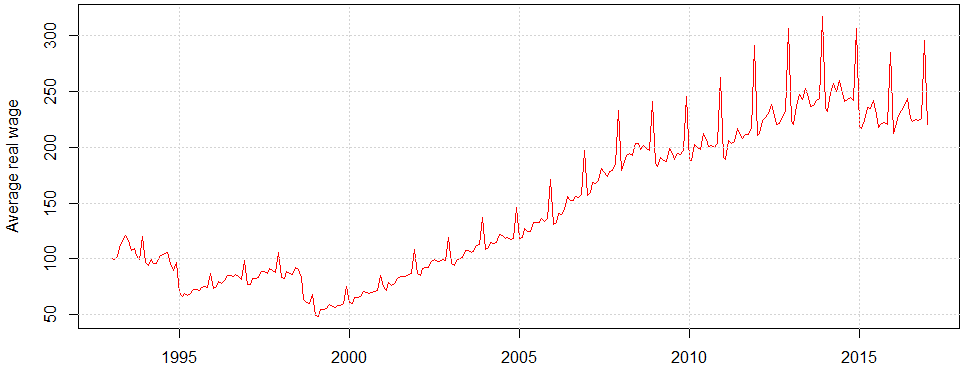
\includegraphics[width=0.7\textwidth]{wage.png}
\end{center}


% Характерными отличиями временного ряда от пространственных выборок являются:
\begin{itemize}
    \item $Y_t$ не являются одинаково распределенными;
    \item $y_t$ статистически зависимы.
\end{itemize}
\end{frame}

\begin{frame}{Виды временных рядов}{По способу выражения}

\begin{itemize}
	\item \textbf{Ряды абсолютных величин}
	\item \textbf{Ряды относительных величин}
	
	{\centering
		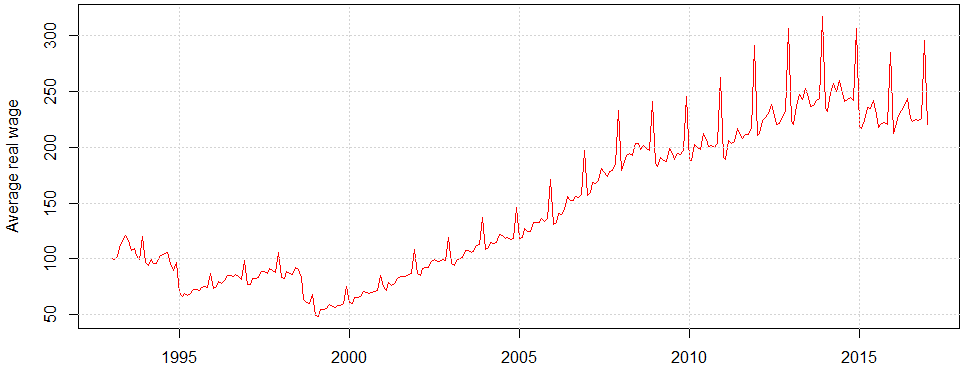
\includegraphics[width=0.65\textwidth]{wage.png}\par
	}

	\item \textbf{Ряды средних величин}
		
	{\centering
		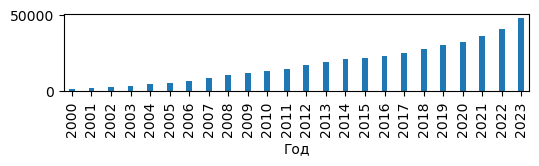
\includegraphics[width=0.65\textwidth]{wage_kirov.png}\par
	}

\end{itemize}

% Важной особенностью интервальных ВР абсолютных величин является возможность суммирования их уровней.  
% В результате получаются накопленные временные ряды, имеющие осмысленное содержание и лишенные проблемы повторного счета.  
% 
% Суммирование уровней моментного ВР чаще всего бессмысленно. Например, суммируя почасовой временной ряд почасовые объемы выручки в течение суток получмаем посуточный временной ряд, но просуммировав число посетителей кафе в 18:00 за неделю мы не сможем получить какой-то осмысленной информации.
% 

\end{frame}


\begin{frame}{Виды временных рядов}{По способу регистрации}

\begin{itemize}
	\item \textbf{Моментные:} ряды значений показателя по состоянию на определенные моменты времени. 
	\begin{itemize}
		\item цена на определененный вид товаров
		\item курс акций
		\item численность населения
		\item число посетителей
	\end{itemize}
	\item \textbf{Интервальные:} ряды накопленных показателей за определенные время:
	\begin{itemize}
		\item объем продаж
		\item численность населения
		\item число посетителей
	\end{itemize}
	\item \textbf{Производные:} ряды, полученные из наблюдаемых данных некоторыми преобразованиями
\end{itemize}

% Важной особенностью интервальных ВР абсолютных величин является возможность суммирования их уровней.  
% В результате получаются накопленные временные ряды, имеющие осмысленное содержание и лишенные проблемы повторного счета.  
% 
% Суммирование уровней моментного ВР чаще всего бессмысленно. Например, суммируя почасовой временной ряд почасовые объемы выручки в течение суток получмаем посуточный временной ряд, но просуммировав число посетителей кафе в 18:00 за неделю мы не сможем получить какой-то осмысленной информации.
% 

\end{frame}

\begin{frame}{Виды временных рядов}{По свойству параметра времени}
\begin{multicols}{2}
\textbf{Нерегулярные (разнесенные во времени):} сбор данных в произвольные моменты времени
	
	{\centering
	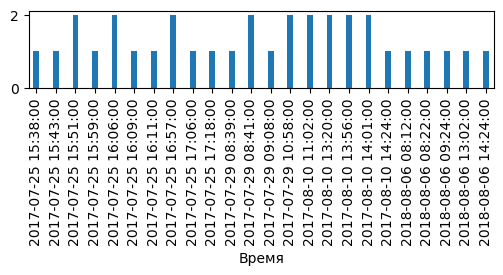
\includegraphics[width=0.45\textwidth]{fish.png}\par
	}

	% данные, полученные в произвольные моменты времени:
	\begin{itemize}
	\item суммы средств, снятых через банкомат
	\item поток данных от систем мониторинга
	%  Нерегулярный временной ряд может иметь длительные периоды без данных или короткие периоды с пакетами данных.
	\end{itemize}
	
	\columnbreak
	
	\textbf{Регулярные (равноотстоящие):} сбор данных через равные промежутки времени

	{\centering
		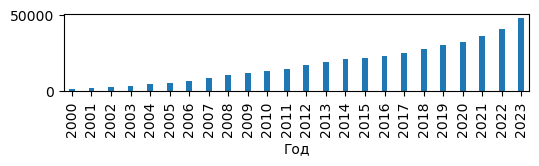
\includegraphics[width=0.48\textwidth]{wage_kirov.png}\par
	}
	
	\textbf{Дискретность}~--- длина промежутка между соседними значениями регулярного ВР
\end{multicols}
	
	% Если дискретность ряда велика, можно упустить существенные закономерности в динамике показателя. Например, по квартальным данным невозможно судить о месячных сезонных колебаниях. 
	% Слишком малая дискретность ряда приводит к увеличению влияния случайностей, маскирующих . 
	% 
	% Вопрос о выборе дискретности временного ряда должен решаться, исходя из целей каждого конкретного исследования.
\end{frame}




\subsection{Общая математическая модель временного ряда}
\begin{frame}{Общая математическая модель временного ряда}{}

Статистическая характеристика случайного дискретный процесс $Y(\omega,t)$~--- совместная функция распределения случайных величин:
$$
	F(Y_1, Y_2, \ldots, Y_t, \ldots)
$$

\medskip
Бесконечное число моментов времени?
% При рассмотрении временного ряда число случайных величин велико и может быть бесконечным. 
% Поэтому, чтобы задать все вероятностные свойства этой конструкции, нам нужна совокупность функций распределения, а именно одномерная функция распределения, двумерная функция распределения и так далее: 

$$
	F_1 \left(Y_{t_1}\right), 
	\quad 
	F_2 \left(Y_{t_1}, Y_{t_2}\right),
	\quad
	F_3 \left(Y_{t_1}, Y_{t_2}, Y_{t_3}\right),
	\ldots
$$
% Индексы величин $x_{t_1}, x_{t_2}$ означают, что случайные величины рассматривается в моменты времени  $t_1, t_2$ и так далее, и у них есть совместная функция распределения. 

% При этом в другие моменты времени функция распределения будет другая. 

% Такая совокупность функций распределения полностью характеризует случайный процесс. 

Функции распределения  согласованы:

% Эта совокупность функций согласована между собой в следующем смысле. Каждую функцию распределения размерности $n$ можно получить из функции распределения размерности $n+1$. 
% Для этого надо проинтегрировать функцию большей размерности по всем значениям одной из переменной.

$$
	F_n(y_{t_1}, \ldots, y_{t_n}) = 
	\int\limits_{y \in Y_{t_{n+1}}} F_{n+1}(Y_{t_1}, \ldots, Y_{t_n}, Y_{t_{n+1}})
$$

Как это получить из временного ряда?
% На практике, как правило, имеется один единственный отрезок реализации стохастического процесса~--- временной ряд, поэтому говорить об оценивании совокупности всех функций распределения не приходится. 
% Кроме того, интуитивно понятно, что если основные статистические характеристики со временем меняются, то мы по короткому кусочку наших наблюдений вообще ничего не сможем сказать о нем. 

% Поэтому на стохастические процессы, порождающие исследуемые временные ряды накладывают дополнительные ограничения. 

% Например, можно предположить, что функция распределения (или плотность распределения) стохастического процесса является композицией детерминированных функций и белого шума.

% Другим подходом является рассмотрение стационарных стохастических процессов. 
\end{frame}


\section{Задачи исследования временного ряда}
\begin{frame}{Задачи исследования временных рядов}
	\begin{itemize}
		\item Прогнозирование развития явления
		\item Характеристика отдельных изменений в уровнях ряда 
		\item Определение средних показателей
		\item Выявление закономерностей динамики исследуемого явления
		\item Выявление факторов, обусловливающих изменение изучаемого объекта во времени
	\end{itemize}
\end{frame}


\subsection{Задача прогнозирования временного ряда}
\begin{frame}{Задача прогнозирования временного ряда}
%%%%%%%%%%%%%%%%%%%%%%%%%%%%%%%%%%%%%%%%%%%%%%%%%%%%%%%%%%%%%%%%%%%%%%%
% В определении временного ряда нужно обратить внимание на то, что временные интервалы между измерениями признака постоянны. Если мы не просто не знаем, чему будет в будущем равно значение признака, но и за какой период оно будет измерено, то такую задачу к прогнозированию ряда свести нельзя.
% Примеры временных рядов — это ряды среднедневных цен на акции определённой компании, среднемесячного уровня безработицы, измеренного в течение нескольких лет, среднегодового уровня производства автомобилей. 
%%%%%%%%%%%%%%%%%%%%%%%%%%%%%%%%%%%%%%%%%%%%%%%%%%%%%%%%%%%%%%%%%%%%%%%
	Регулярный временной ряд: $y_1,\dots,y_T,\dots,\;\; y_t\in\mathbb{R},$
	
	\begin{center}
		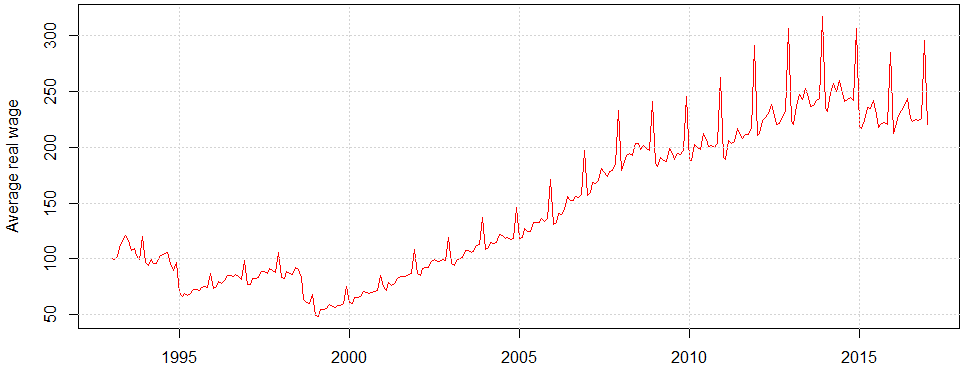
\includegraphics[width=0.65\textwidth]{wage.png}
	\end{center}
	
	\textbf{Задача прогнозирования}~--- найти функцию $f_T\colon$
	$$
	y_{T+d} \approx f_T\left(y_1,\ldots,y_T, d\right) \equiv \hat{y}_{T+d|T},$$
	где 
	\begin{itemize}
		\item $d \in \left\{1,\dots,D\right\}$~--- прогнозный лаг, 
		\item $D$~--- горизонт прогнозирования.		
	\end{itemize}
	
\end{frame}

\begin{frame}{Регрессия}
%%%%%%%%%%%%%%%%%%%%%%%%%%%%%%%%%%%%%%%%%%%%%%%%%%%%%%%%%%%%%%%%%%%%%%%
% До этого, на протяжении практически всего курса, считалось, что анализируемые данные — это простые выборки, то есть независимые одинаково распределённые наблюдения. В задаче анализа временных рядов всё с точностью наоборот: предполагается, что данные в прошлом каким-то образом связаны с данными в будущем. Чем сильнее они связаны, тем больше имеется информации о поведении временного ряда в будущем и тем точнее можно сделать прогноз.
% Как этот прогноз построить? Мы хорошо умее делать регрессию. Процесс разворачивается во времени, поэтому кажется логичным задать признак, связанный со временем, и попробовать решить задачу, применяя модель регрессии. Признак может зависеть от вермени линейно, или например, квадратично.
% Однако это решение слишком простое, чтобы быть хорошим. Остатки такой регрессии далеко не похожи на случайный шум, в них остаётся большая часть структуры, которая не была учтена в регрессионной модели. Чем больше структуры временного ряда учитывается в модели, тем лучшее предсказание она даёт. Вид остатков регрессии намекает на то, что можно построить более сложную модель, которая будет лучше описывать имеющиеся данные, а также давать более точные прогнозы в будущем.
%%%%%%%%%%%%%%%%%%%%%%%%%%%%%%%%%%%%%%%%%%%%%%%%%%%%%%%%%%%%%%%%%%%%%%%
	Сделаем регрессию на время?
	\begin{center}
		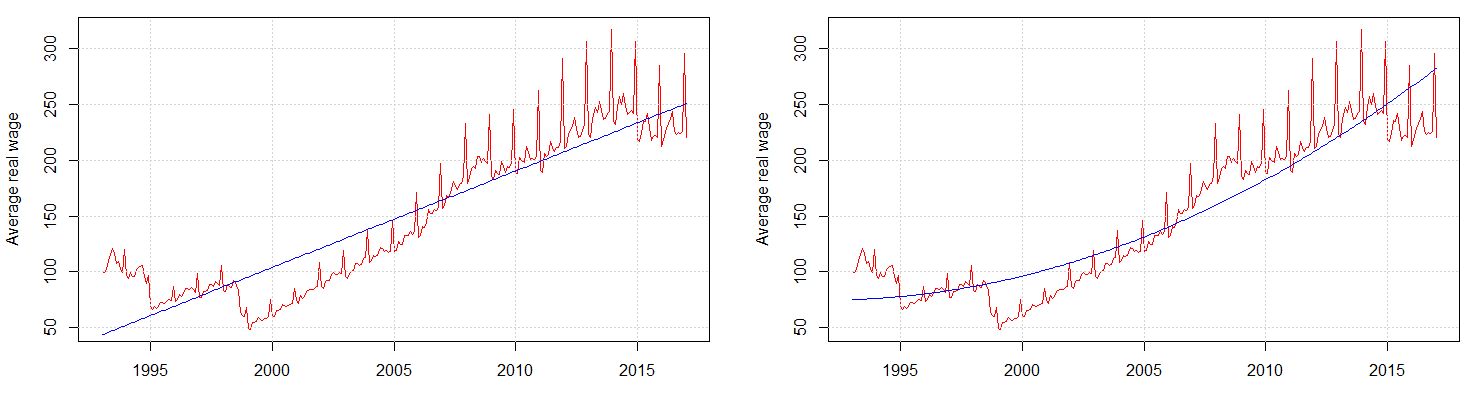
\includegraphics[width=0.9\textwidth]{wage1.png}
	\end{center}		
	
	Остатки содержат информацию!
	\begin{center}
		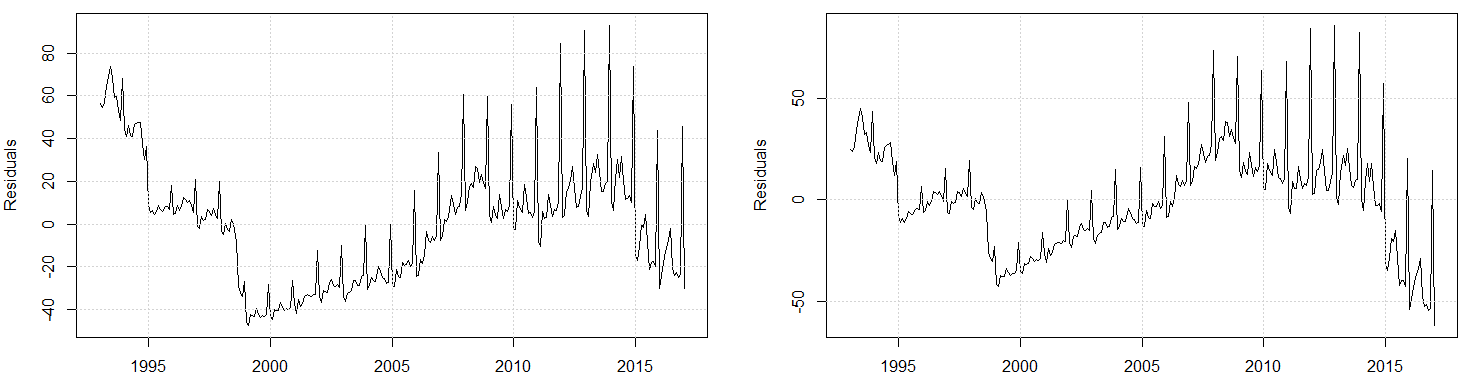
\includegraphics[width=0.9\textwidth]{wage2.png}
	\end{center}			
\end{frame}


\begin{frame}{Характеристика отдельных изменений в уровнях ряда}{Показатели ВР}
	\renewcommand{\arraystretch}{2}	
	\begin{tabular}{p{5cm}cc}
		& \textbf{Базисный} & \textbf{Цепной}  \\
	\hline
	\textbf{Абсолютный прирост} $\Delta y_i$ &
		$\Delta y_i^{\text{б}} = y_i-y_0$ & 
		$\Delta y_i^{\text{ц}} = y_i-y_{i-1}$ \\
	\textbf{Темп роста} $T y_i$ & 
		$T y_i^{\text{б}} =\dfrac{y_i}{y_0}$ & 
		$T y_i^{\text{ц}} = \dfrac{y_i}{y_{i-1}}$\\
	\textbf{Темп прироста} $\Delta T y_i$ & 
		$\Delta T y_i^{\text{б}} = \dfrac{\Delta y_i^{\text{б}}}{y_0} = T y_i^{\text{б}}-1$ & 
		$\Delta T y_i^{\text{ц}} = \dfrac{\Delta y_i^{\text{ц}}}{y_{i-1}} = T y_i^{\text{ц}}-1$\\
	\textbf{Темп наращивания} $T_\text{н} y_i$&
	\multicolumn{2}{c}{$T_\text{н} y_i = \dfrac{\Delta y_i^{\text{ц}}}{y_0}$}\\ 
	\textbf{Абсолютное значение одного процента прироста} $A_i$&
	\multicolumn{2}{c}{$A_i =  \dfrac{\Delta y_i^{\text{ц}}}{100 \cdot \Delta T y_i^{\text{ц}}} y_i = 0.01y_{i-1}$}\\ 	
\end{tabular}
\end{frame}

\begin{frame}{Определение средних показателей уровней ВР}{Показатели ВР}
	
	\renewcommand{\arraystretch}{2}	
	\begin{tabular}{lcc}
		& \textbf{Регулярный} & \textbf{Нерегулярный} \\
		\textbf{Интервальный ВР} &
		$\displaystyle \bar{y} = \frac{1}{n}\sum\limits_{i=1}^{n} y_i$
		&
		$\displaystyle \bar{y} = \frac{\sum\limits_{i=1}^{n} y_i \Delta t_i}{\sum\limits_{i=1}^{n} \Delta t_i }$
		\\
		\textbf{Моментный ВР} &
		$\displaystyle \bar{y} = \frac{1}{n-1}\sum\limits_{i=1}^{n-1} \frac{y_i+y_{i+1}}{2}$ &
		$\displaystyle \bar{y} = \frac{\sum\limits_{i=1}^{n-1} \frac{y_i+y_{i+1}}{2} \Delta t_i }{\sum\limits_{i=1}^{n-1} t_i}$
		\\	
	\end{tabular}

	\bigskip
	\structure{Средние показатели изменения уровней ВР}

	\renewcommand{\arraystretch}{2}	
	\begin{tabular}{ccc}
		Средний абсолютный прирост & Средний темп роста & Средний темп прироста \\
		$\displaystyle \Delta\bar{y} = \frac{1}{n}\sum\limits_{i=1}^{n-1} \Delta y_i^{\text{ц}}$ &		
		$\displaystyle \overline{T y} = \sqrt[n]{\prod_{i=1}^{n-1} T y_i^{\text{ц}}} = \sqrt[n]{\frac{y_n}{y_1}}$ & 
		$\displaystyle \overline{ \Delta T y} = \overline{ \Delta T y} - 1$
		\\
	\end{tabular}
\end{frame}

\begin{frame}{Показатели вариации ВР}{Показатели ВР}
	
	\renewcommand{\arraystretch}{2}	
	\begin{tabular}{>{\bfseries}lc}
		Размах  уровней: &
		$\displaystyle \delta_i = |y_i - \bar{y}|$
		\\
		Среднее линейное отклонение ряда: &
		$\displaystyle d = \frac{1}{n}\sum_{i=1}^{n} \delta_i$
		\\
		Среднее квадратичное отклонение: &
		$\displaystyle \sigma = \sqrt{\frac{1}{n}\sum_{i=1}^{n} \delta^2_i}$
		\\
		Коэффициент вариации: & 
		$\displaystyle V = \frac{\sigma}{\bar{y}}$
		\\
	\end{tabular}
\end{frame}


\begin{frame}{Автокорреляционная функция (ACF)}{}
%%%%%%%%%%%%%%%%%%%%%%%%%%%%%%%%%%%%%%%%%%%%%%%%%%%%%%%%%%%%%%%%%%%%%%%
% Одной из важнейших характеристик временного ряда является автокорреляция, измеряющая в каком-то смысле сходство между значениями ряда в соседних точках. Автокорреляция — это уже встречавшаяся ранее корреляция Пирсона между исходным рядом и его версией, сдвинутой на несколько отсчётов. Количество отсчётов, на которое сдвинут ряд, называется лагом автокорреляции. Значения, принимаемые автокорреляцией такие же, как и у коэффициента Пирсона: [-1; 1]. Проверить, значимо ли отличие автокорреляции от нуля, можно с помощью такого же критерия Стьюдента, как используется для корреляции Пирсона.
%%%%%%%%%%%%%%%%%%%%%%%%%%%%%%%%%%%%%%%%%%%%%%%%%%%%%%%%%%%%%%%%%%%%%%%
	Сопоставим каждому лагу $\tau$ значение коэффициента корреляции между временным рядом $Y_t$ и $Y_{t-\tau}$
	$$
		\rho_\tau  
		=  \frac{\mathop{\mathrm{Cov}} (Y_t,Y_{t+\tau})}{D(Y_t)} 
		= \frac{\sum\limits_{t=1}^{n-\tau} \left(y_t - \bar{y}\right)\left(y_{t+\tau} - \bar{y}\right) }{ \sum\limits_{t=1}^n \left(y_t - \bar{y}\right)^2 }\in\left[-1,1\right],
	$$
		
		\bigskip
		
		\structure{Проверка значимости отличия автокорреляции от нуля}:
		\begin{center}
			\begin{tabular}{rl}
				временной ряд:                  & $Y^T = Y_1,\dots,Y_n$ \\
				гипотезы:               & $H_0\colon r_\tau=0, \qquad H_1\colon r_\tau \neq 0 $ \\
				статистика:                     & $\displaystyle T\left(Y^T\right) = \frac{r_{\tau} \sqrt{T-\tau-2}}{\sqrt{1-r_\tau^2}};$ \\
				нулевое распределение:          & $St\left(T-\tau-2\right)$.\\
			\end{tabular}
		\end{center}
\end{frame}

\begin{frame}{Коррелограмма}{}
	\begin{center}
		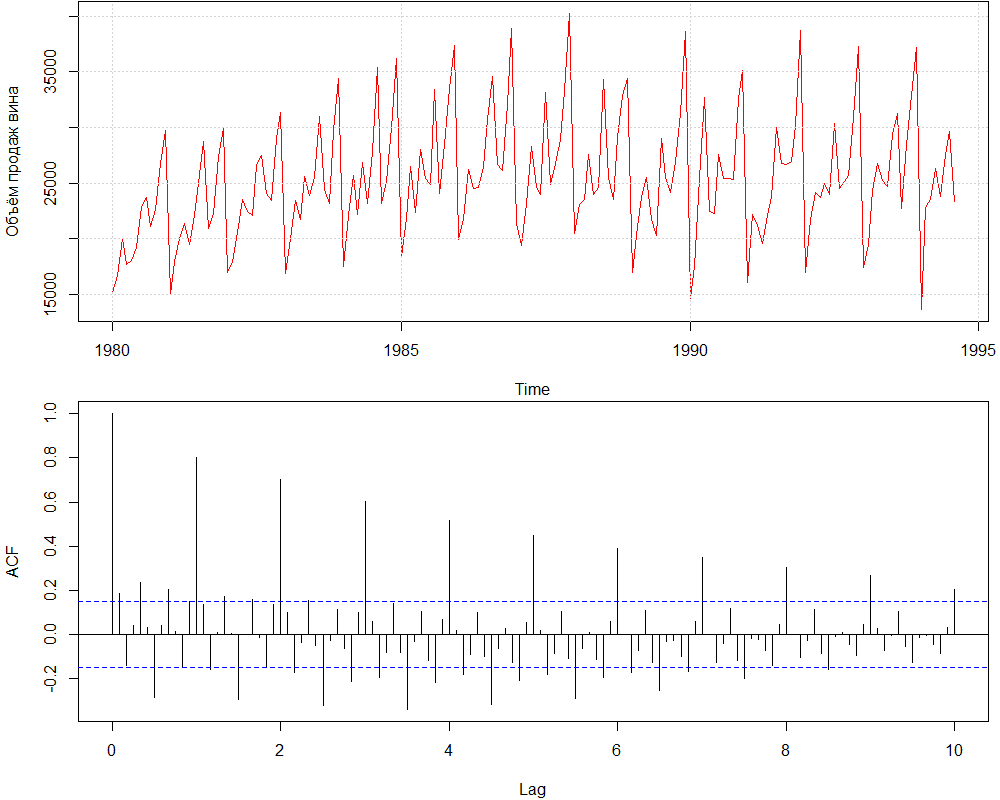
\includegraphics[height=0.85\textheight]{wineacf.png}
	\end{center}				
\end{frame}
\begin{frame}{Частная автокорреляционная функция PACF}{partial autocorrelation function}
	$PACF(\tau)$~--- МНК оценка коэффициента $\alpha_\tau$ в регрессии:
 $$
    Y_t = \alpha_0 + \alpha_1 Y_{t-1} +   \alpha_2 Y_{t-2} +  \alpha_\tau Y_{t-\tau} + \varepsilon_t
 $$

%  Исходя из экономического смысла коэффициента линейной регрессии при предикторе $Y_{t-\tau}$ при 
Частная автокорреляция $PACF(\tau)$ показывает «чистую» зависимость между уровнями $Y_t$ и $Y_{t-\tau}$ временного ряда при исключении влияния промежуточных значений.
\end{frame}
\subsection{Декомпозиция временного ряда}
\begin{frame}{Компоненты временных рядов}
%%%%%%%%%%%%%%%%%%%%%%%%%%%%%%%%%%%%%%%%%%%%%%%%%%%%%%%%%%%%%%%%%%%%%%%
% Рассмотрим несколько понятий, которыми можно описать поведение временных рядов:
% Тренд — плавное долгосрочное изменение уровня ряда. Эту характеристику можно оценить, наблюдая ряд в течение достаточно долгого времени.
% Сезонность — циклические изменения уровня ряда с постоянным периодом. В данных о средней зарплате в России очень хорошо видны подобные сезонные колебания: признак всегда принимает максимальное значение в декабре каждого года, а минимальное — в январе следующего года. В целом профиль изменения зарплаты внутри года остаётся более-менее постоянным.
% Цикл — измеменение уровня ряда с переменным периодом. Такое поведение часто встречается в рядах, связанных с продажами, и объясняется циклическими изменениями экономической активности. В экономике выделяют циклы длиной 4 - 5 лет, 7 - 11 лет, 45 - 50 лет и т. д. Другой пример ряда с такой характеристикой — это солнечная активность, которая соответствует, например, количеству солнечных пятен за день. Она плавно меняется с периодом, который составляет несколько лет, причём сам период также меняется во времени.
% Шум — непрогнозируемая случайная компонента ряда. Сюда включены все те характеристики временного ряда, которые сложно измерить (например, слишком слабые).
%%%%%%%%%%%%%%%%%%%%%%%%%%%%%%%%%%%%%%%%%%%%%%%%%%%%%%%%%%%%%%%%%%%%%%%
	\begin{description}[\textbf{Цикличность} $v_t$]
		\item[\textbf{Тренд} $u_t$]~--- плавное долгосрочное изменение уровня ряда.
		
		\item[\textbf{Сезонность} $s_t$]~--- циклические изменения уровня ряда с постоянным периодом.
		
		\item[\textbf{Цикличность} $v_t$]~--- изменения уровня ряда с переменным периодом 
		\begin{itemize}
			\item цикл жизни товара, 
			\item экономические волны,
			\item периоды солнечной активности
		\end{itemize}		
		\item[\textbf{Остатки} $\varepsilon_t$]~--- непрогнозируемая случайная компонента ряда.
	\end{description}

	\bigskip
	\bigskip
	\structure{\Large Декомпозиция ВР:}
	
	\bigskip
	{\centering

	\renewcommand{\arraystretch}{2}	
	\begin{tabular}{ccc}
		\textbf{Аддитивная} & \textbf{Мультипликативная} & \textbf{Смешанная}
		\\
		\structure{$y_t = u_t+s_t+v_t+\varepsilon_t$} 
		&
    	\structure{$y_t = u_t\cdot s_t \cdot v_t \cdot \varepsilon_t$}
		& 
		\structure{$y_t = u_t\cdot s_t \cdot v_t + \varepsilon_t$}
		\\
	\end{tabular}
	\par
	}
\end{frame}


\begin{frame}{Примеры, содержащие компоненты}
%%%%%%%%%%%%%%%%%%%%%%%%%%%%%%%%%%%%%%%%%%%%%%%%%%%%%%%%%%%%%%%%%%%%%%%
% Левый верхний график - суммарный объём проданной жилой недвижимости в Америке за месяц, данные собраны за несколько лет. На графике наблюдается сочетание двух основных компонент. Первая компонента — это годовая сезонность (минимум всегда приходится на зиму, а максимум — на середину лета), а вторая — это циклы, связанные с изменением среднего уровня экономической активности (период в данном случае составляет 7-9 лет).
% 
% Правый верхний график - количество контрактов за день в сокровищнице США. На графике виден хорошо выраженный нисходящий тренд, который можно описать линейной функцией. На этом участке в данных не наблюдается ни циклов, ни сезонности. По-видимому, всё, что не удаётся описать трендом, является ошибкой.
% 
% Слева внизу данные за несколько лет о суммарном объёме электричества, произведённого за месяц в Австралии. На графике, как и в предыдущем случае, виден тренд, на этот раз повышающийся. Кроме того, наблюдается годовая сезонность: значение признака совершает колебания, минимум которых всегда приходится на зиму, а максимум — на середину лета. Это легко объяснить тем, что зимой электричества необходимо меньше всего, это самый тёплый сезон в Австралии.
% 
% Справа внизу ежедневные изменения индекса Доу-Джонса. Глядя на этот график, сложно сказать, присутствует ли в данных какая-то систематическая компонента: явно нет ни тренда, ни сезонности, ни цикла. По всей видимости, ряд представляет собой что-то похожее на случайные колебания. Однако даже такие ряды можно прогнозировать.
%%%%%%%%%%%%%%%%%%%%%%%%%%%%%%%%%%%%%%%%%%%%%%%%%%%%%%%%%%%%%%%%%%%%%%%
		\begin{center}
			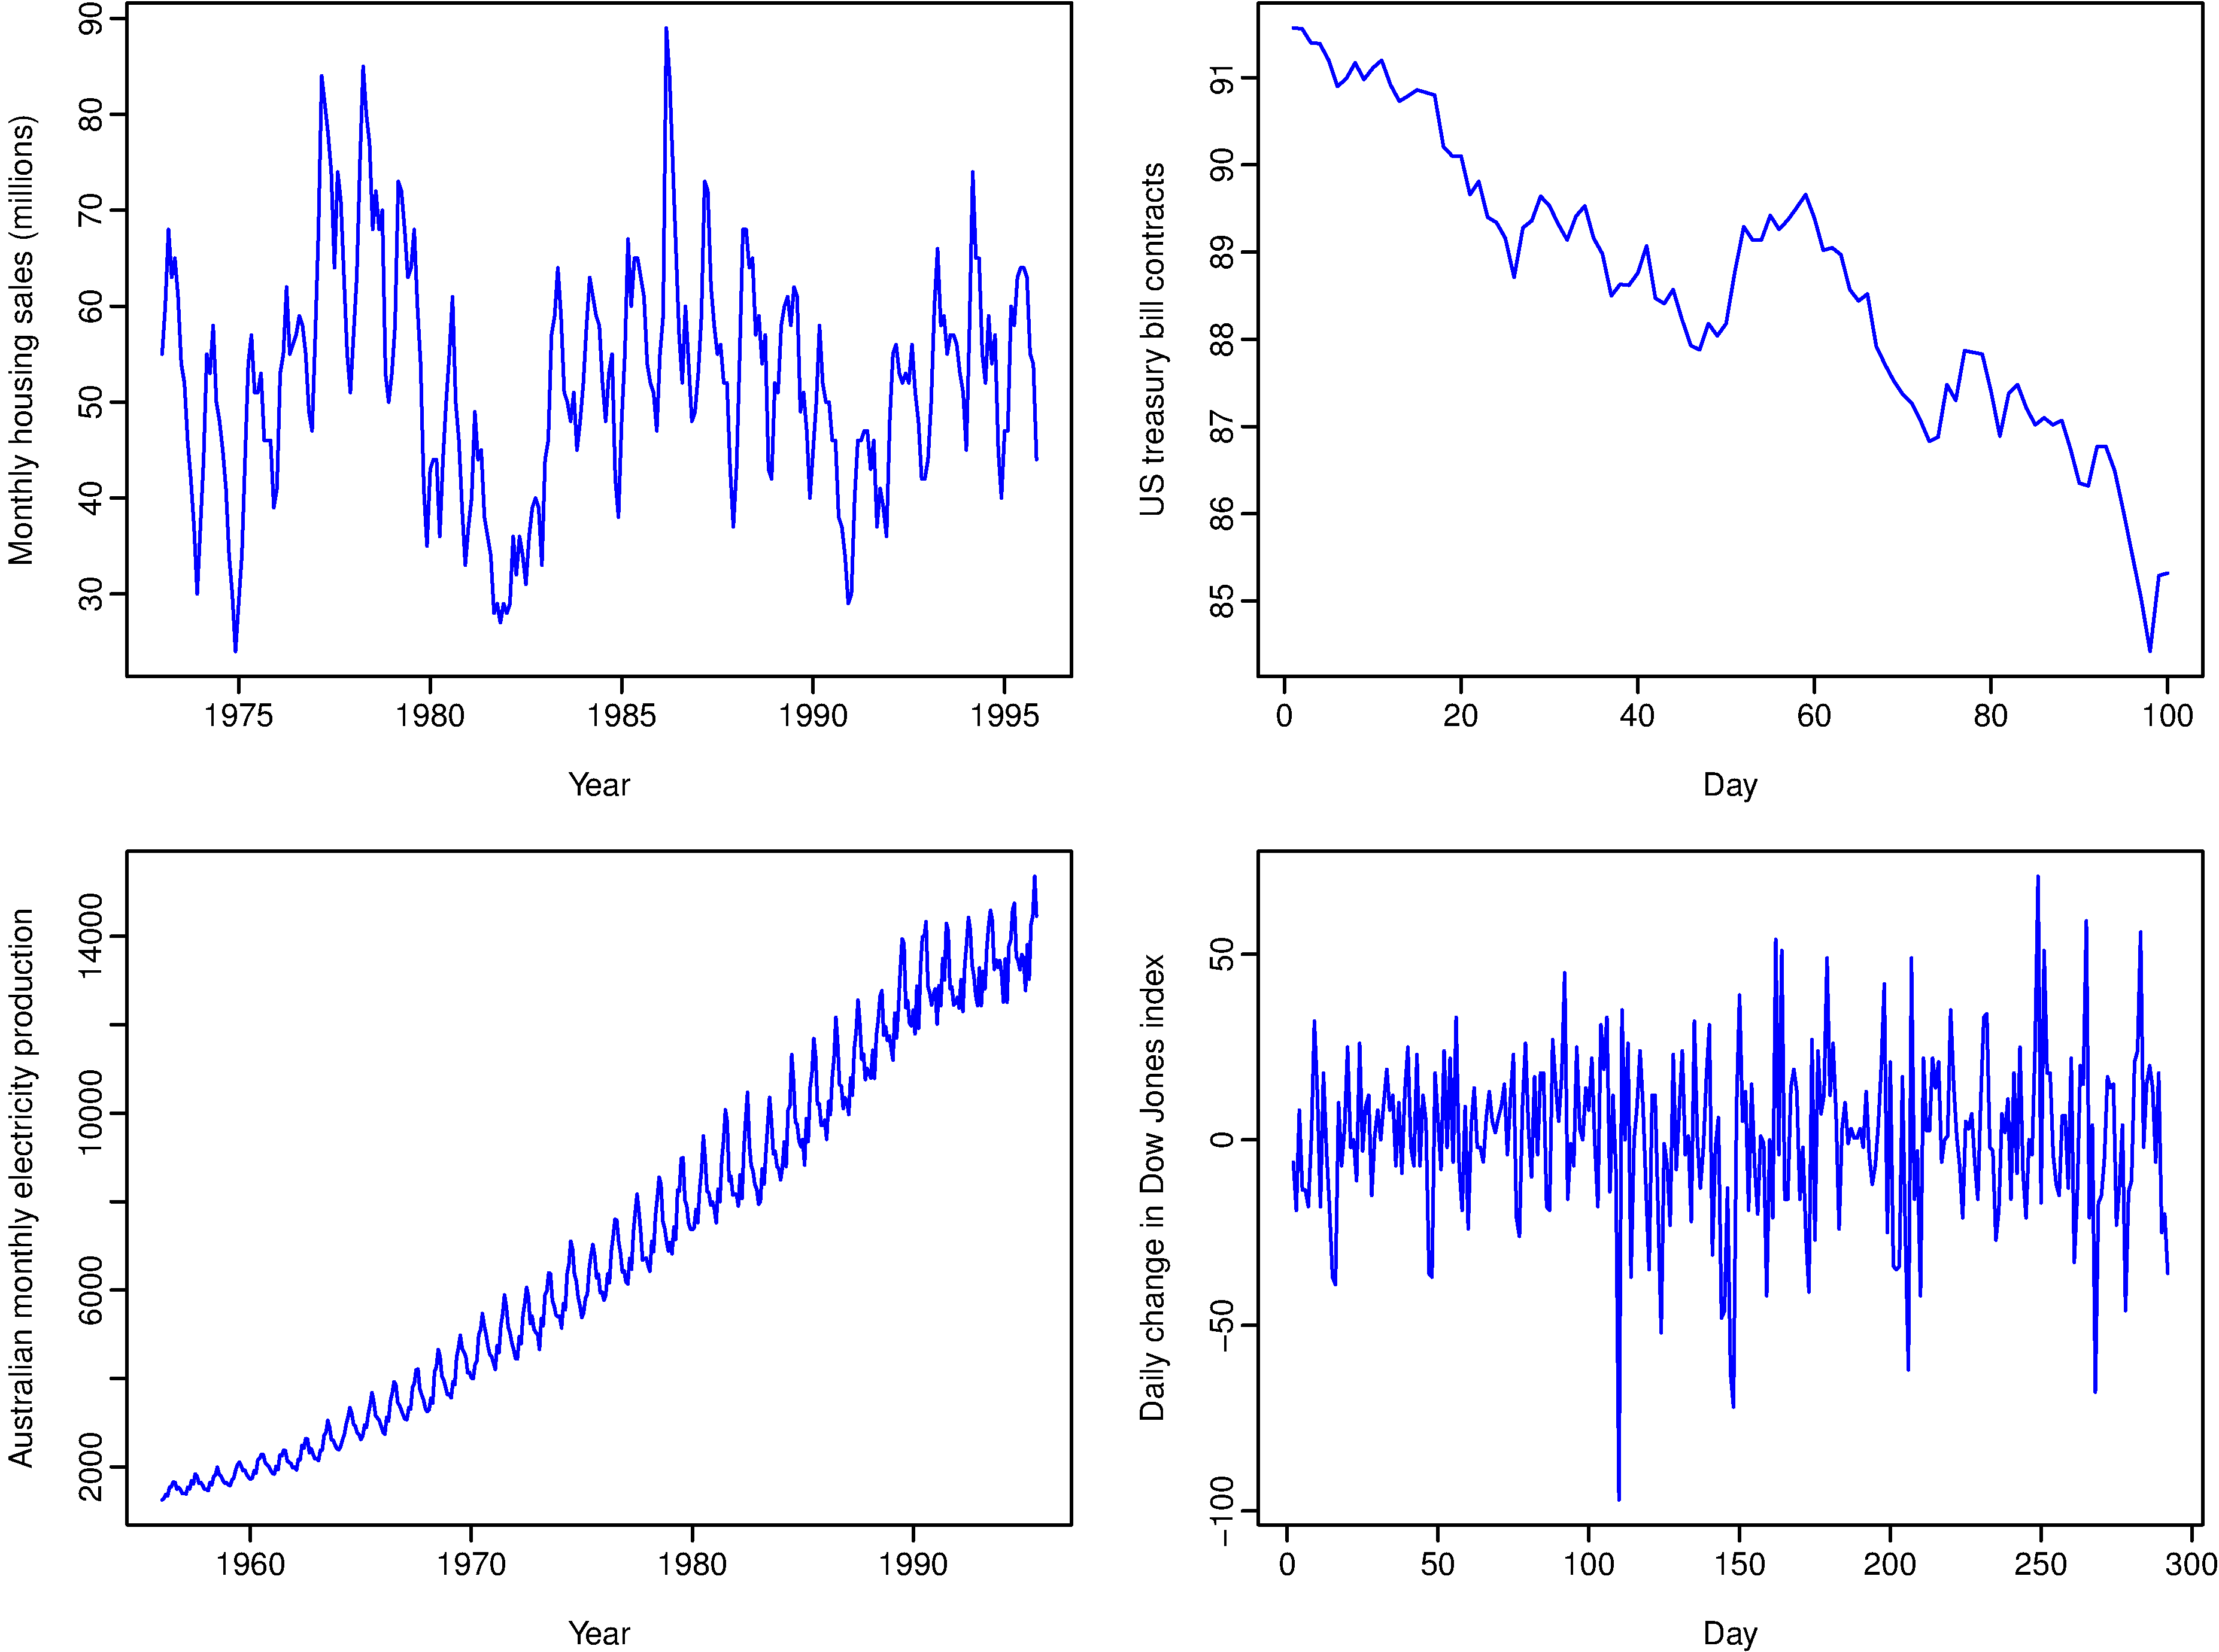
\includegraphics[width=0.8\textwidth]{decomp1.png}
		\end{center}		
\end{frame}

\begin{frame}[fragile]{Метод STL-декомпозиции}
%%%%%%%%%%%%%%%%%%%%%%%%%%%%%%%%%%%%%%%%%%%%%%%%%%%%%%%%%%%%%%%%%%%%%%%	
% STL-декомпозиция - простой эвристический метод оценки разных компонент временного ряда: на верхнем графике исходныя ряд, потом сезонность (ей разрешается немного меняться), потом тренд и ошибка.
%%%%%%%%%%%%%%%%%%%%%%%%%%%%%%%%%%%%%%%%%%%%%%%%%%%%%%%%%%%%%%%%%%%%%%%	
		\begin{multicols*}{2}
			\begin{center}
				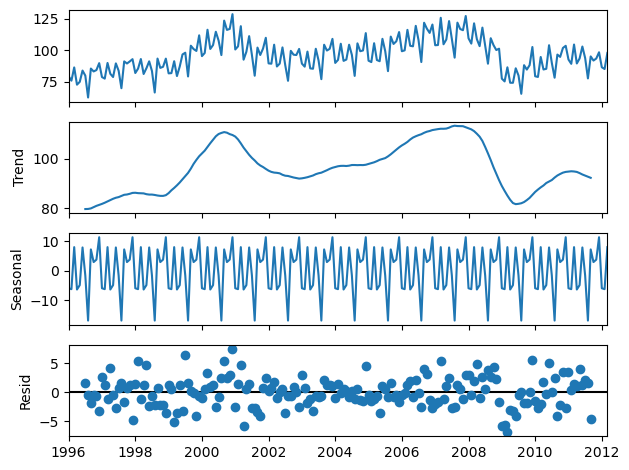
\includegraphics[height=0.6\textheight]{elecequip_stl.png}
			\end{center}			
		\columnbreak
	
		\footnotesize
		\begin{verbatim}
from statsmodels.tsa.seasonal \
	import seasonal_decompose
elecequip = pd.read_csv('elecequip.csv')
elecequip.set_index('Index', inplace=True)

decompose = seasonal_decompose(
	elecequip, 
	model = 'additive', 
	period=12)

trend = decompose.trend
seasonal = decompose.seasonal
residual = decompose.resid

decompose.plot();			
		\end{verbatim}
		\let\thefootnote\relax\footnotetext{\texttt{https://github.com/antoinecarme/TimeSeriesData/raw/refs/heads/master/fpp2/elecequip.csv}}
		\end{multicols*}
\end{frame}


\begin{frame}{Компоненты временных рядов}
%%%%%%%%%%%%%%%%%%%%%%%%%%%%%%%%%%%%%%%%%%%%%%%%%%%%%%%%%%%%%%%%%%%%%%%
% Давайте теперь посмотрим, как на коррелограммах проявляются разные компоненты временных рядов. Вернёмся к коррелограмме ряда продаж вина в Австралии. На графике видно, что автокорреляция принимает большие значения в лагах, кратных сезонному периоду. Такой вид коррелограммы типичен для данных с выраженной сезонностью.
%%%%%%%%%%%%%%%%%%%%%%%%%%%%%%%%%%%%%%%%%%%%%%%%%%%%%%%%%%%%%%%%%%%%%%%
		\begin{center}
			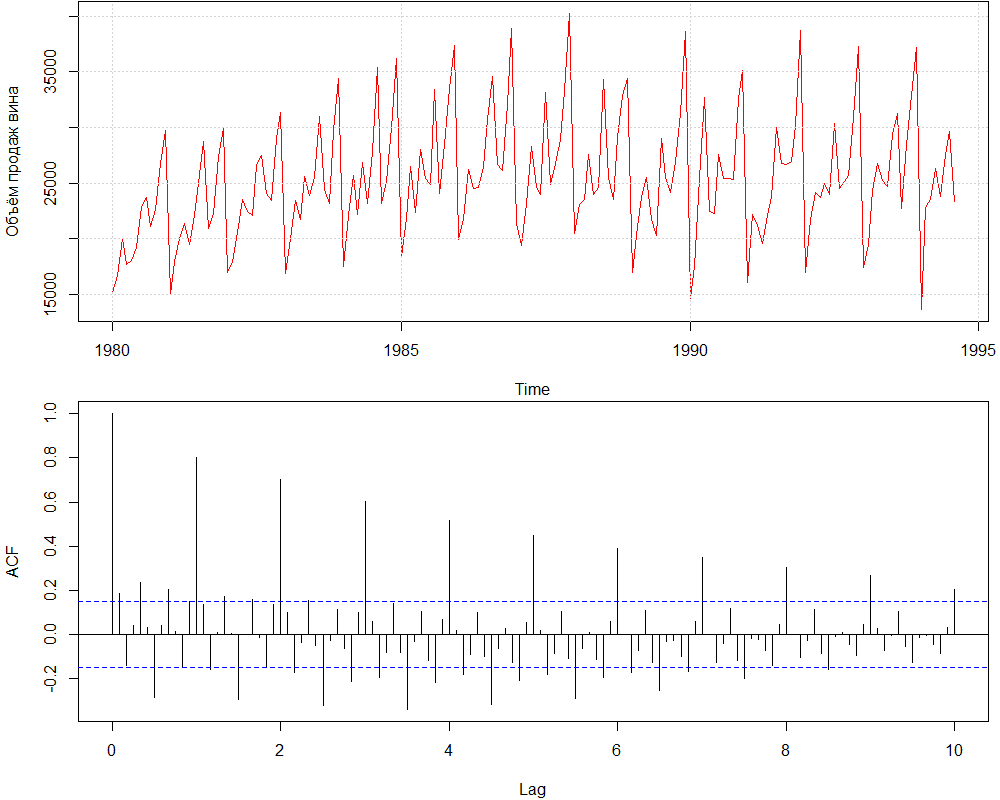
\includegraphics[height=0.7\textheight]{wineacf.png}
		\end{center}				
\end{frame}

\begin{frame}{Компоненты временных рядов}
%%%%%%%%%%%%%%%%%%%%%%%%%%%%%%%%%%%%%%%%%%%%%%%%%%%%%%%%%%%%%%%%%%%%%%%
% На этом слайде коррелограммы для четырёх только что рассмотренных рядов.
% Левый верхний график - типичная коррелограмма для ряда, в котором есть и сезонность, и цикл. Для самого первого лага, кратного сезонному периоду, виден пик, однако далее положение этого пика смещается: следующий пик не приходится на 2, 3 или 4 года. Это происходит, потому что в ряде есть циклы, период которых плавно меняется.
% Правый верхний график - типичная коррелограмма для данных с ярко выраженным трендом. Автокорреляция тем больше, чем меньше величина лага, и с ростом лага она начинает постепенно убывать, при  этом автокорреляция может начать колебаться вокруг горизонтальной оси, соответствующей её нулевому значению.
% В ряде слева внизу в котором присутствуют и тренд, и сезонность. Таким образом, на ней можно наблюдать оба описанных ранее эффекта, однако тренд настолько сильный, что практически нейтрализует влияние сезонности (следствие которой — наличие пиков в лагах, кратных периоду сезона).
% На коррелограмме, соответствующей данным о ежедневном изменении индекса Доу-Джонса, все значения автокорреляции невелики, кроме первого (в данной точке лаг = 0, и вычисляется корреляция значения ряда с самим собой, а такая корреляция всегда равна 1).
%%%%%%%%%%%%%%%%%%%%%%%%%%%%%%%%%%%%%%%%%%%%%%%%%%%%%%%%%%%%%%%%%%%%%%%	
		\begin{center}
			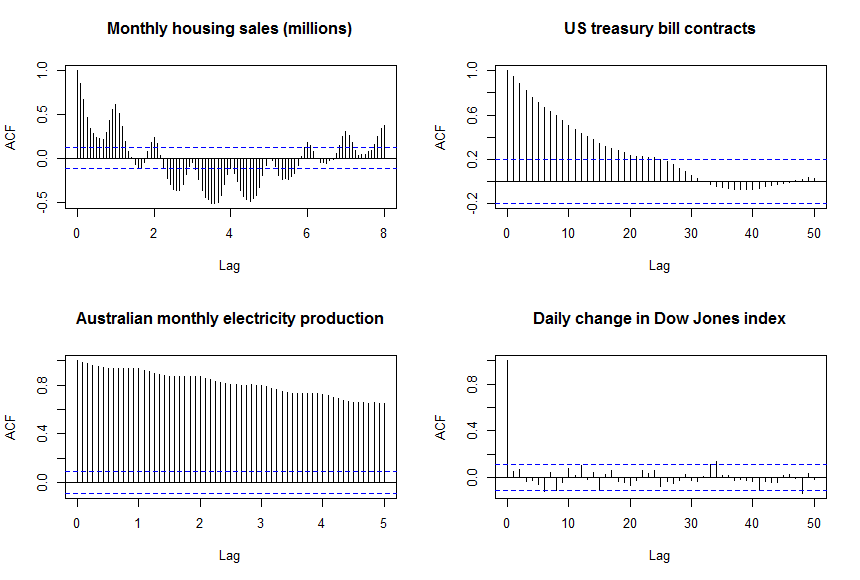
\includegraphics[width=0.8\textwidth]{acfs.png}
		\end{center}		
\end{frame}




\subsection{Определение тренда}
\begin{frame}{Метод  разности средних}{Проверка наличия тренда}
	Предполагается, что данные временного ряда нормально распределены.
	\begin{enumerate}
		\item Временной ряд разбивают на две примерно равные по числу уровней части.
		\item  Вычисляются средние значения и выборочные дисперсии 
		\item Проверяется гипотеза о равeнстве дисперсий с помощью F-критерия Фишера. Если гипотеза отвергается, то метод не применим.
		\item Проверяется гипотеза о равeнстве средних. Если гипотеза отвергается, то имеет место тернд.
	\end{enumerate}
	По этому методу  (в первой части
n1 первых уровней исходного ряда, во второй остальные n2=n-n1 уровней).
Каждая из частей рассматривается как самостоятельная
выборочная
совокупность, имеющая нормальное распределение. Для каждой из этих частей
вычисляются средние значения и дисперсии:
\end{frame}

\begin{frame}{Метод Фостера"--~Стьюарта}{Проверка наличия тренда}
	\begin{enumerate}
		\item Для $t= \overline{2,n}$ определяются две числовые последовательности:
		$$
			g_t = [\forall i<t\; (y_t > y_i)], 
			\qquad
			l_t = [\forall i<t\; (y_t < y_i)], 
		$$

		\item  Вычисляются две величины:
		$$
		d = \sum_{t=2}^n (g_t-l_t),\qquad
		s = \sum_{t=2}^n (g_t+l_t)
		$$
		Обе величины асимптотически нормальны и имеют независимые
		распределения.
		\item Для обнаружения тренда в среднем проверяется $H_0\colon d=0$:
		$$
		t_d = \frac{|d|}{\sigma_2}\sim St(\alpha,n-1),
		 \qquad 
		 \sigma_2 = \sqrt{2\sum_{t=2}^n \frac{1}{t}}
		$$
		\item Для обнаружения тренда в дисперсии проверяется гипотеза $H_0\colon s=\bar{y}$:
		$$
		t_s = \frac{|s-\bar{y}|}{\sigma_1}\sim St(\alpha,n-1),
		 \qquad 
		 \sigma_1 = \sqrt{2\sum_{t=2}^n \frac{1}{t}-4\sum_{t=2}^n \frac{1}{t^2}}
		$$
	\end{enumerate}
\end{frame}

\begin{frame}{Метод аналитического выравнивания}{Выделение тренда}
	\begin{multicols}{2}
	\structure{Идея:} Задать трендовую компоненту функцией.
	
	\medskip
	
	{\centering
	\renewcommand{\arraystretch}{1.2}	
	\begin{tabular}{lc}
		Вид зависимости & Формула\\
		\hline
		Линейная & $u(t) = a+bt$\\
		Квадратическая& $u(t) = a+bt+ct^2$\\
		Обратная & $u(t) = a+\frac{b}{t}$\\
		Степенная & $u(t) = a+t^b$\\
		Показательная & $u(t) = a+b^t$\\
		Экспоненциальная & $u(t) = a+e^{bt}$\\
	\end{tabular}
	\par}
	\columnbreak
	\structure{Как выбрать?}
	\begin{itemize}
		\item метод Тинтнера\footnote{\href{http://elibrary.asu.ru/xmlui/bitstream/handle/asu/8717/book.pdf}{Саженкова Т.В.  Пономарёв И.В., Пронь 	С.П. Методы анализа временных рядов: учебно-методическое пособие. Барнаул: Изд-во Алт. ун-та. 2020. С. 34}}
	\item метод характеристик прироста 
	\end{itemize}

	\bigskip
	\structure{Алгоритм:}
	\begin{enumerate}
		\item Выбирается вид функциональной зависимости 
		\item формируется модель $y_t  = u(t) + \varepsilon_t$
		\item Путем решения задачи регрессии $y_t=u(t)$ определяются коэффициенты~$u_{t}$.
		\item Выделяется тренд $u_t = u(t)$
	\end{enumerate}
	\end{multicols}
	
	
\end{frame}

\begin{frame}{Метод  скользящего среднего МСС (SMA - simple moving average)}{Сглаживание ряда; Выделение тренда}
	\structure{Идея:} сопоставить значению уровня $y_i$~--- среднее арифметическое предыдущих значений.\footnote{pandas.DataFrame.rolling().mean()}
	$$
		M_t = \frac{1}{m} \sum_{i=t-m+1}^{t} y_i 
		\quad \text{ или }\quad
		M_t = \frac{1}{m} 
		\sum_{i=t-\lceil m/2 \rceil}^{t+\lfloor m/2 \rfloor} y_i
	$$

	{
		\centering
		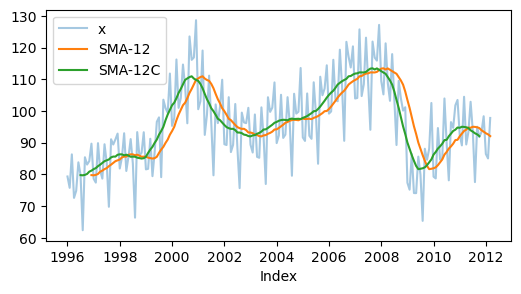
\includegraphics[width=0.65\textwidth]{sma12.png}
		\par
	}
\end{frame}

\begin{frame}{Выравнивание ВР }{}
	Выравнивание временного ряда  --- удаление трендовой компоненты:

	{\centering
		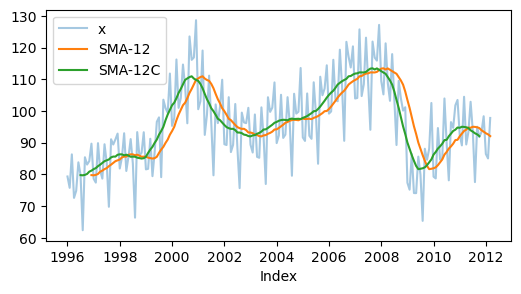
\includegraphics[width=0.55\textwidth]{sma12.png}
		\par
		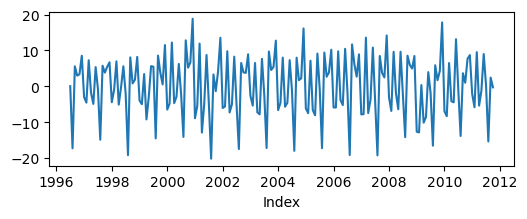
\includegraphics[width=0.55\textwidth]{sma12_detrend.png}
		\par
	}

\end{frame}

% \section{Выделение сезонности}
% \begin{frame}{Снятие сезонности}
% 	Часто для удобства интерпретации ряда сезонная компонента вычитается:	
% 	\begin{center}
% 		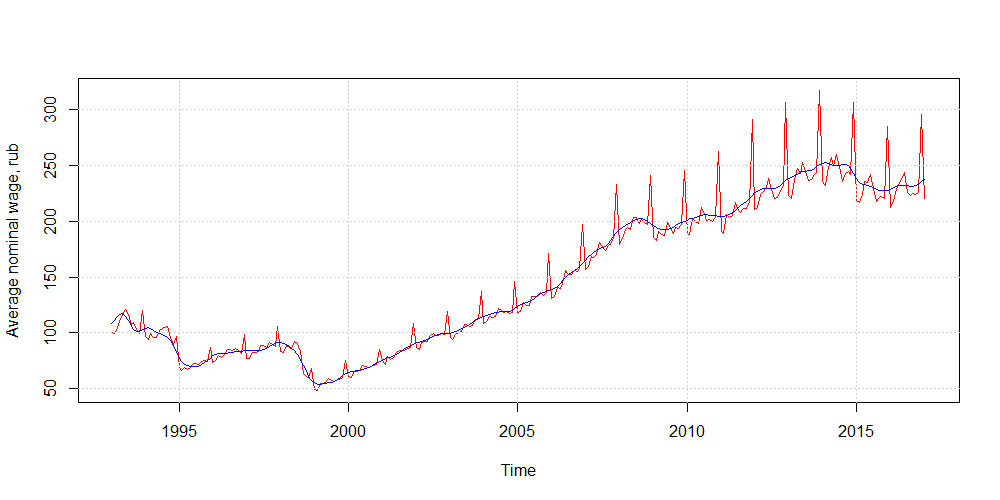
\includegraphics[width=.8\textwidth]{wageseas.png}
% 	\end{center}	
% \end{frame}

% \begin{frame}{Календарные эффекты}
% %%%%%%%%%%%%%%%%%%%%%%%%%%%%%%%%%%%%%%%%%%%%%%%%%%%%%%%%%%%%%%%%%%%%%%%	
% % Часто отсчёты временного ряда имеют разную абсолютную длину, например, если это месяцы. Если ряд имеет смысл суммарного количества чего-нибудь, то оказывается, что его структуру можно сильно упростить, если на эту длину поделить. Такой ряд оказывается проще прогнозировать, а в интерпретации мы при этом ничего не теряем. Иногда срабатывает деление не на количество дней, а на количество рабочих дней в периоде. Выбрать способ такого упрощения можно исходя из здравого смысла.
% %%%%%%%%%%%%%%%%%%%%%%%%%%%%%%%%%%%%%%%%%%%%%%%%%%%%%%%%%%%%%%%%%%%%%%%	
% 	Иногда упростить структуру временного ряда можно за счёт учёта неравномерности отсчётов:
	
% 	\begin{center}
% 		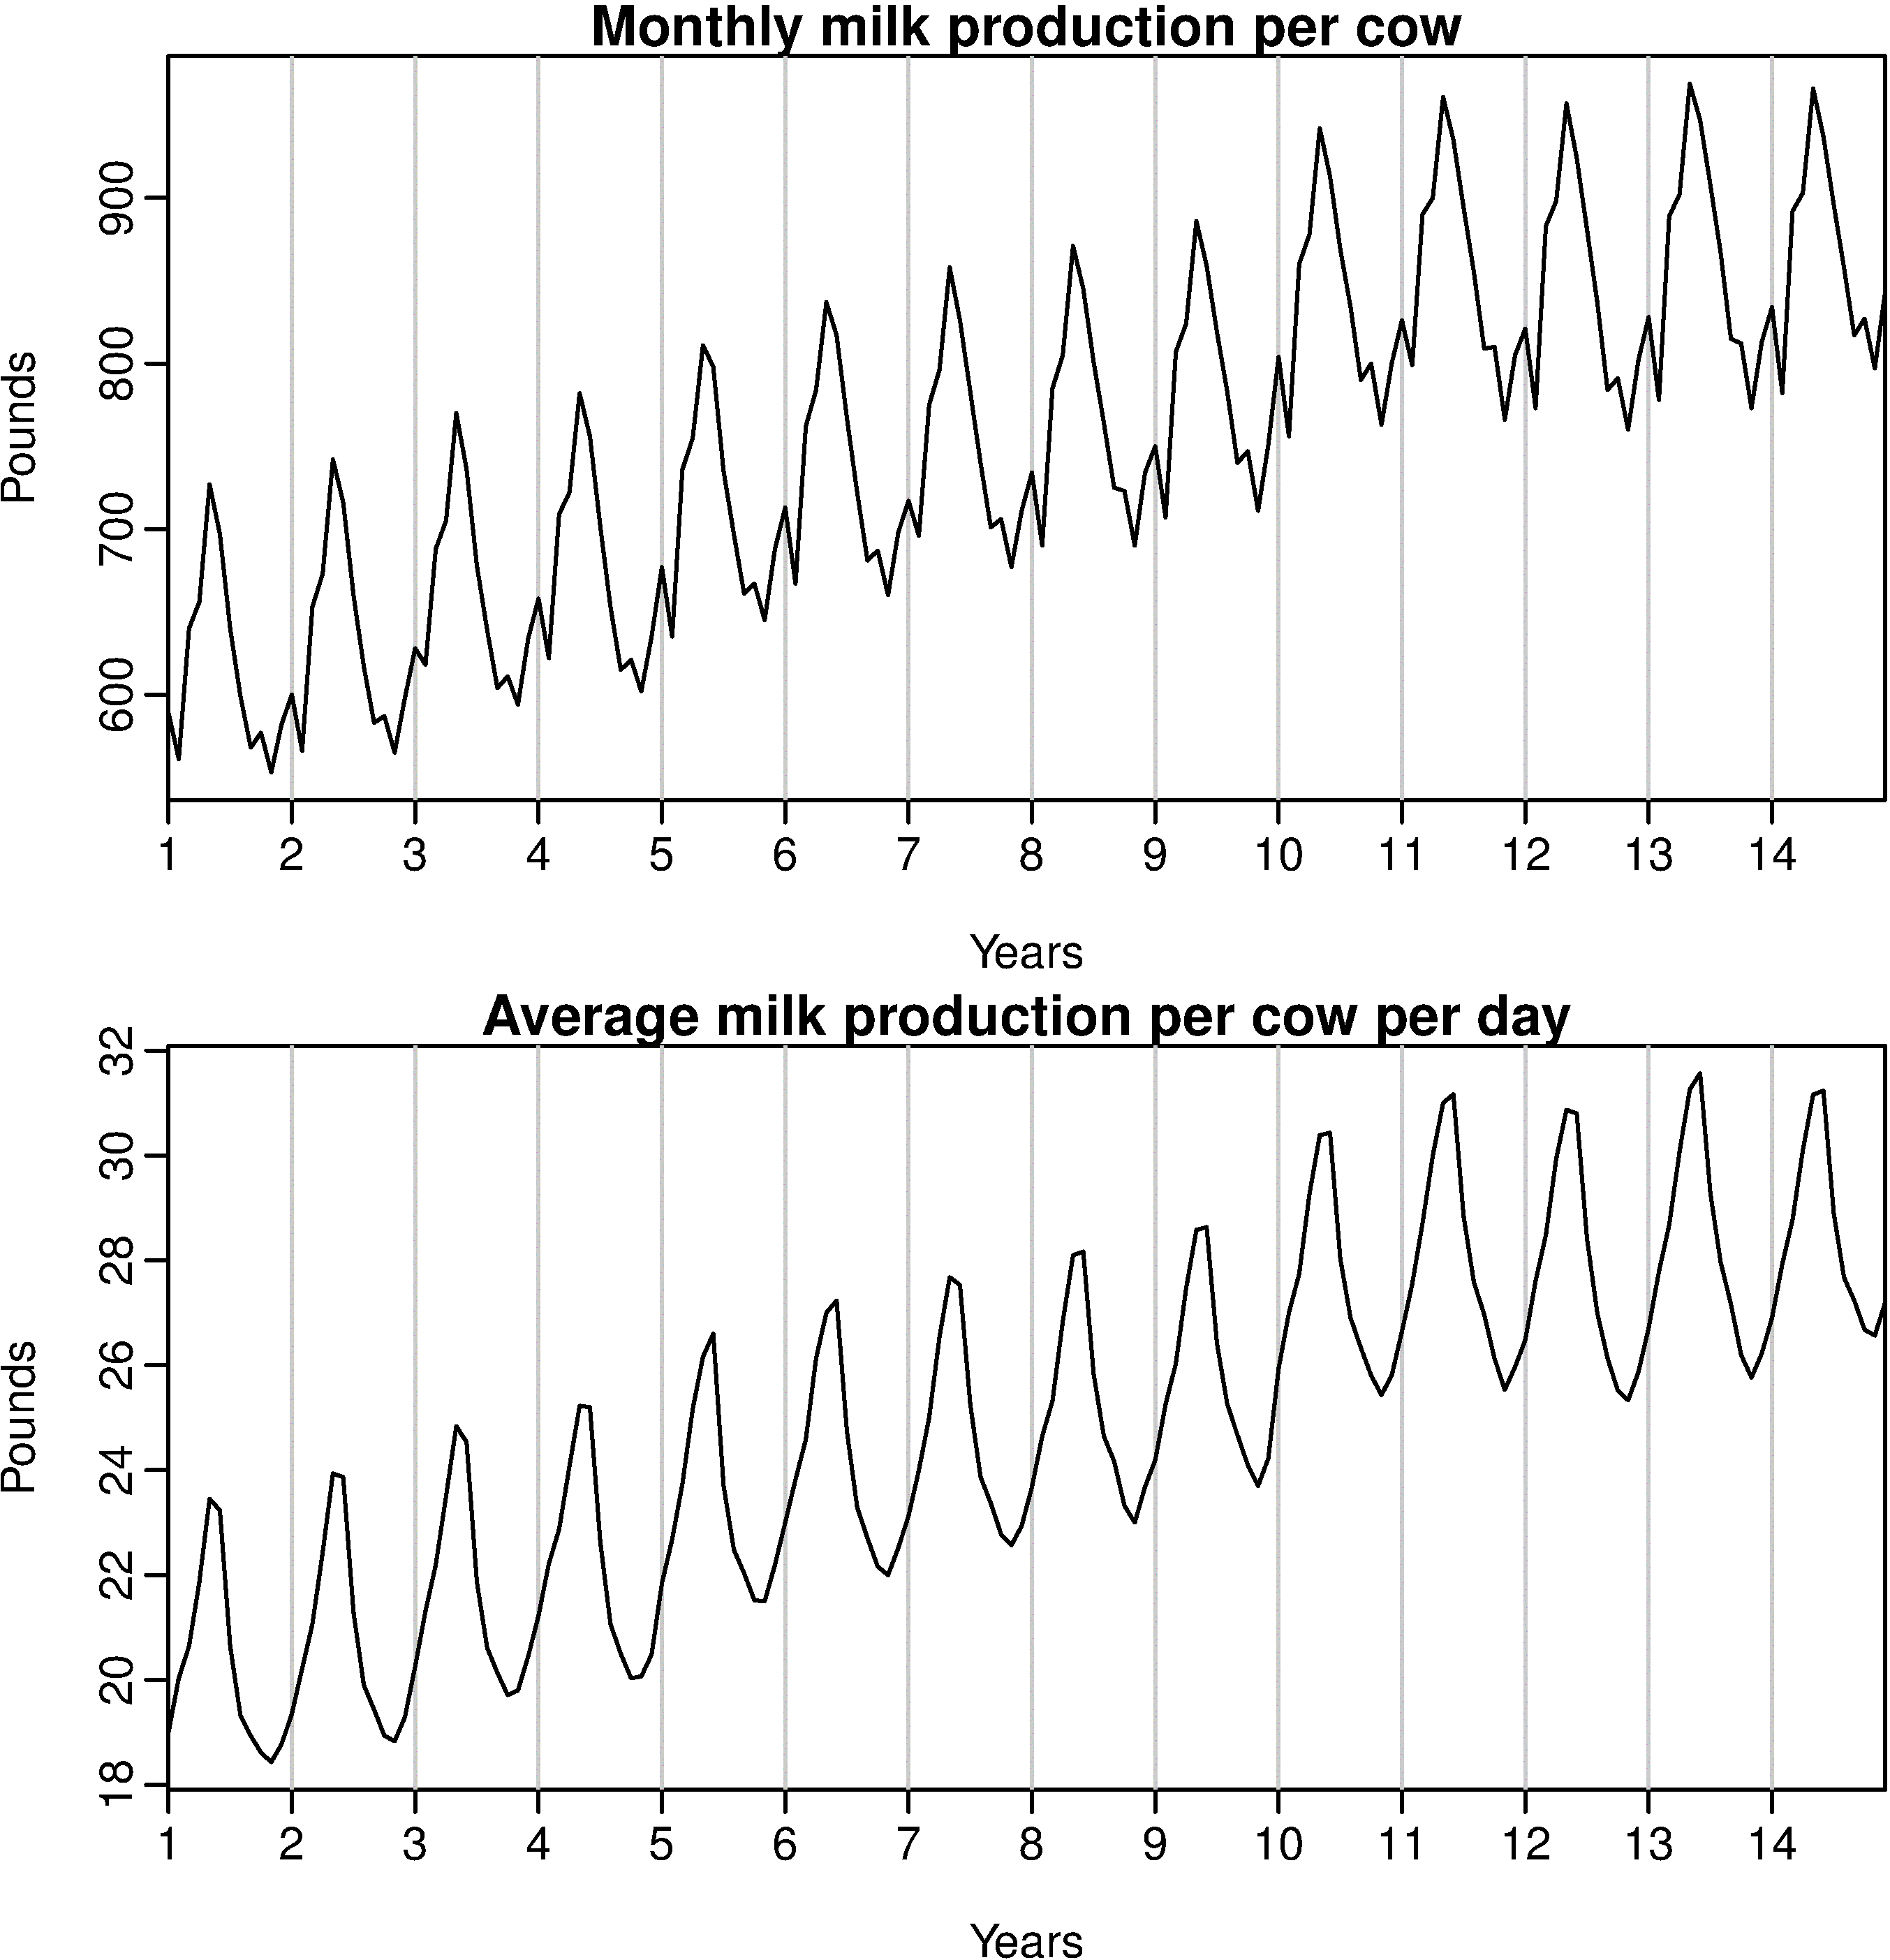
\includegraphics[height=0.6\textheight]{milk.png}
% 	\end{center}
% \end{frame}




\section{Модели экспоненциального сглаживания}



\begin{frame}{Простейшие методы прогнозирования}
	\begin{itemize}
		\item средним:
		$$\hat{y}_{T+d} = \frac1{T}\sum_{t=1}^T y_t;$$
		\item средним за последние $k$ отсчётов:
		$$\hat{y}_{T+d} = \frac1{k}\sum_{t=T-k}^T y_t;$$
		\item наивный:
		$$\hat{y}_{T+d} = y_T;$$
		\item наивный сезонный ($s$~--- период сезонности):
		$$\hat{y}_{T+d} = y_{T+d-ks}, \; k = \lfloor\left(d-1\right)/s\rfloor+1;$$
		\item экстраполяции тренда:
		$$\hat{y}_{T+d} = y_T + d \frac{y_T-y_1}{T-1}.$$
	\end{itemize}
\end{frame}

\begin{frame}{Идея метода Брауна}

		Метод взвешенного среднего: 
		$$
			M_{t} = \sum_{i=0}^{m-1} w_iy_{t-i}, \qquad \sum_{i=0}^{m-1} w_i=1.
		$$
		Возьмем в качестве весов геометрическую убывающую последовательность:
		$$
		\hat{y}_{t} 
		= \alpha y_t 
		+ \alpha \left(1-\alpha\right)y_{t-1} 
		+ \alpha \left(1-\alpha\right)^2y_{t-2}
		+\ldots
		$$

		Рекуррентная форма \textbf{экспоненциального сглаживания}:
		$$
  			\alert{l_t = \alpha y_t + (1-\alpha) l_{t-1}}
		$$
	$\alpha$~--- \textbf{параметр сглаживания}
	\begin{itemize}
		\item $\alpha \to 1$~--- больший вес последним точкам,
		\item $\alpha \to 0$~--- большее сглаживание.
	\end{itemize}		
		\bigskip
		
		{\scriptsize
			\begin{table}[h]
				\begin{tabular}{|c|c|c|c|c|}
					\hline
					Наблюдение & $\alpha=0.2$ & $\alpha=0.4$ & $\alpha=0.6$ & $\alpha=0.8$ \\\hline
					$y_T$      & $0.2$        & $0.4$        & $0.6$        & $0.8$        \\
					$y_{T-1}$  & $0.16$       & $0.24$       & $0.24$       & $0.16$       \\
					$y_{T-2}$  & $0.128$      & $0.144$      & $0.096$      & $0.032$      \\
					$y_{T-3}$  & $0.1024$     & $0.0864$     & $0.0384$     & $0.0064$     \\
					$y_{T-4}$  & $0.08192$    & $0.05184$    & $0.01536$    & $0.00128$    \\
					$y_{T-5}$  & $0.065536$   & $0.031104$   & $0.006144$   & $0.000256$   \\
					\hline
				\end{tabular}
			\end{table}	
		}	
\end{frame}
\begin{frame}{Прогнозированипе методом Брауна}
	
Для прогнозирования рекуррентная формула может быть переписана в следующем виде:
$$
  \hat{y}_{T+1|T} = \alpha y_T + (1-\alpha) \hat{y}_{T}
$$


		\begin{itemize}
			\item Метод подходит для прогнозирования рядов без тренда и сезонности:
			\begin{align*}
			\hat{y}_{t+1|t} &= l_t, \\
			l_t &= \alert{\alpha} y_t + \alert{\left(1-\alpha\right)}l_{t-1}=\hat y_{t|t-1} + \alert{\alpha\cdot e_t}.
			\end{align*}
%    \[
%        \hat y_{t+1} := \alert{\alpha} y_t + \alert{(1-\alpha)} \hat y_{t}= \hat y_{t} + \alert{\alpha\cdot e_t}
%    \]
%
    $e_t = y_t-\hat{y}_{t|t-1}$~--- ошибка прогноза отсчёта времени $t$


			\item Прогноз зависит от $l_0$:
			$$\hat{y}_{T+1|T} = \sum_{j=1}^{T-1}\alpha\left(1-\alpha\right)^j y_{T-j} + \left(1-\alpha\right)^T l_0.$$
			Можно взять $l_0=y_1$ или оптимизировать его.
			\item Прогноз получается \emph{плоский}, т.\,е. $\hat{y}_{t+d|t} = \hat{y}_{t+1|t}$.
		\end{itemize}
\end{frame}
\begin{frame}{Метод Брауна. Пример}
		\begin{center}
			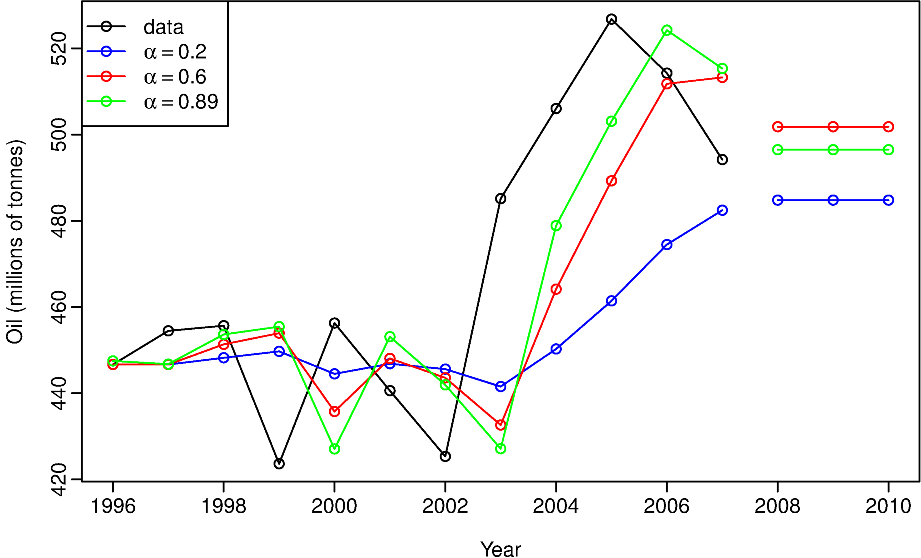
\includegraphics[width=0.6\textwidth]{fig_7_ses}
		\end{center}
		Простое экспоненциальное сглаживание в применении к данным о добыче нефти в~Саудовской Аравии (1996–2007)\footnote{\url{https://www.statsmodels.org/stable/examples/notebooks/generated/exponential_smoothing.html}}.
\end{frame}

\begin{frame}{Метод Хольта (двухпараметрический метод сглаживания)}{1957, statsmodels.tsa.holtwinters.Holt(data, damped\_trend=False)}
	\structure{Идея:} Учтем тренд

% 	Если во временных рядах имеется тенденция к росту, то вместе с оценкой текущего уровня необходима и оценка тренда. 
% В методике Хольта значения уровня $L_t$ (level) и тренда $T_t$ (trend) сглаживаются непосредственно, при этом используются различные параметры сглаживания для каждого из них:
% $\alpha$~--- для уровня, $\beta$ для тренда. 
% Преимуществом методики Хольта является возможность выбора соотношения, в котором отслеживаются уровень и тренд.
	\begin{multicols}{2}

		Аддитивный линейный тренд (метод Хольта):
		\begin{align*}
		\hat{y}_{t+d|t} &= l_t + d b_t, \\
		l_{t}       &= \alpha y_t + \left(1-\alpha\right) \left(l_{t-1} + b_{t-1}\right), \\
		b_t         &= \beta \left(l_t - l_{t-1}\right) + \left(1-\beta\right) b_{t-1}.
		\end{align*}
		
		\columnbreak
		
		Мультипликативный линейный (экспоненциальный) тренд:
		\begin{align*}
		\hat{y}_{t+d|t} &= l_tb_t^d, \\
		l_{t}       &= \alpha y_t + \left(1-\alpha\right) \left(l_{t-1} b_{t-1}\right), \\
		b_t         &= \beta \frac{l_t}{l_{t-1}} + \left(1-\beta\right) b_{t-1}.
		\end{align*}
	\end{multicols}
		\bigskip
		
		\bigskip
		\begin{itemize}
			\item $\alpha \in \left[0,1\right]$~--- параметр сглаживания уровня
			\item $\beta \in \left[0,1\right]$~--- параметр сглаживания тренда
		\end{itemize}
		
% Начальные значения обычно берутся следующим образом:$L_1 = y_1$, $T_1 =0$. Иногда, в качестве начального используется среднее значение первых пяти или шести наблюдений.

% Как и при обычном экспоненциальном сглаживании, постоянные $\alpha$ и $\beta$ выбираются субъективно или путем минимизации ошибки прогнозирования. 
% Чем большие значения весов будут взяты, тем более быстрый отклик на происходящие изменения будет иметь место и наоборот, с уменьшением весов реакция модели на изменения в данных будет более слабой.

% Выбор параметров можно осуществлять минимизацией MSE по сетке или градиентным спуском 
Если $\alpha=\beta$, то это \emph{двойное экспоненциальное сглаживание Брауна}.

\end{frame}

\begin{frame}{Метод Хольта с затуханием тренда}{statsmodels.tsa.holtwinters.Holt(data, damped\_trend=True)}
	
	\begin{multicols}{2}
		
		Аддитивный затухающий тренд:
		\begin{align*}
		\hat{y}_{t+d|t} &= l_t + \left(\phi + \phi^2 + \dots + \phi^{d}\right) b_t, \\
		l_{t}       &= \alpha y_t + \left(1-\alpha\right) \left(l_{t-1} +\phi b_{t-1}\right), \\
		b_t         &= \beta \left(l_t - l_{t-1}\right) + \left(1-\beta\right)\phi b_{t-1}.
		\end{align*}
		
		\columnbreak
		
		Мультипликативный затухающий тренд:
		\begin{align*}
		\hat{y}_{t+d|t} &= l_t b_t^{\left(\phi + \phi^2 + \dots + \phi^{d}\right)}, \\
		l_{t}       &= \alpha y_t + \left(1-\alpha\right) l_{t-1} b_{t-1}^{\phi}, \\
		b_t         &= \beta\frac{l_t}{l_{t-1}} + \left(1-\beta\right)b_{t-1}^{\phi}.
		\end{align*}
	\end{multicols}
		
		\bigskip
		\begin{itemize}
			\item $\alpha \in \left[0,1\right]$~--- параметр сглаживания уровня
			\item $\beta \in \left[0,1\right]$~--- параметр сглаживания тренда
			\item $\phi \in \left(0,1\right)$~--- коэффициент затухания.
		\end{itemize}
		
\end{frame}

\begin{frame}{Метод Хольта. Пример}
		\begin{center}
			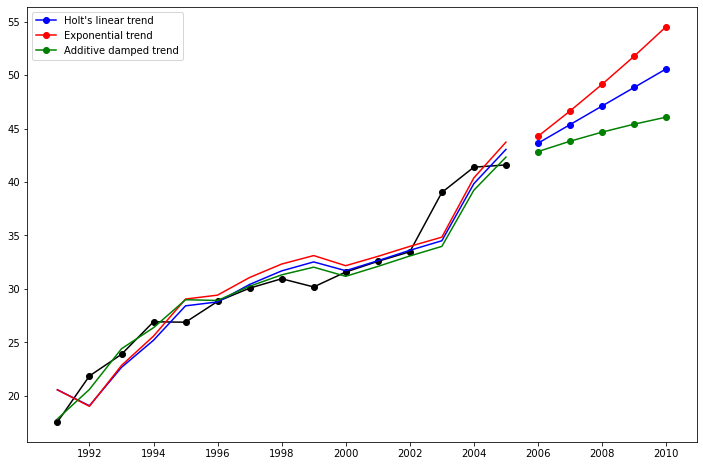
\includegraphics[width=0.65\textwidth]{fig_7_from_statsmodels.png}
		\end{center}
		Прогнозы поголовья овец в Азии с учётом тренда.\footnote{\url{https://www.statsmodels.org/stable/examples/notebooks/generated/exponential_smoothing.html}}
\end{frame}

\begin{frame}{Метод Хольта"--~Винтерса (Трехпараметрическое сглаживание)}{1960, statsmodels.tsa.holtwinters.ExponentialSmoothing}
% Если в структуре данных присутствуют сезонные колебания, то для уменьшения ошибок прогнозирования применяют трехпараметрическую модель экспоненциального сглаживания, предложенную в 1960 году Винтерсом. Этот подход является расширением метода Хольта с помощью дополнительного уравнения учета сезонных колебаний.

	\begin{multicols}{2}
		Аддитивная сезонность c периодом длины~$m$ (метод Тейла"--~Веджа):
		\begin{align*}
		\hat{y}_{t+d|t} &= l_t + d b_t + s_{t-m+\left(d \mod m\right)}, \\
		l_{t}       	&=  \alpha \left(y_t - s_{t-m}\right)+ \left(1-\alpha\right) \left(l_{t-1} + b_{t-1}\right), \\
		b_t         	&= \beta \left(l_t - l_{t-1}\right) + \left(1-\beta\right)b_{t-1}, \\
		s_t         	&= \gamma\left(y_t-l_{t-1}-b_{t-1}\right) + \left(1-\gamma\right)s_{t-m}.
		\end{align*}
		
		\columnbreak
		
		Мультипликативная сезонность (Хольта"--~Винтерса):
		\begin{align*}
		\hat{y}_{t+d|t} &= \left(l_t + d b_t\right)s_{t-m+\left(d \mod m\right)}, \\
		l_{t}           &= \alpha \frac{y_t}{s_{t-m}}+ \left(1-\alpha\right) \left(l_{t-1} + b_{t-1}\right), \\
		b_t             &= \beta \left(l_t - l_{t-1}\right) + \left(1-\beta\right)b_{t-1}, \\
		s_t             &= \gamma\frac{y_t}{l_{t-1}+b_{t-1}} + \left(1-\gamma\right)s_{t-m}.
		\end{align*}

		% Метод Винтерса позволяет наиболее просто учесть в модели сезонность, если исходные данные имеют сезонную структуру. Альтернативой может стать исключение сезонной компоненты либо ее учет в самих данных, например, рассмотрением ряда разностей.
		
	\end{multicols}
\end{frame}

\begin{frame}{Метод Хольта"--~Винтерса. Пример}
		\begin{center}
			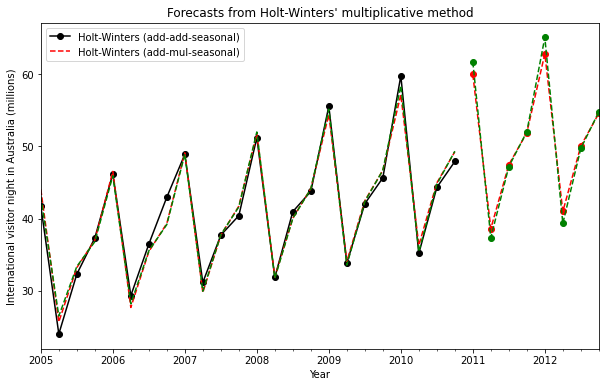
\includegraphics[width=0.5\textwidth]{fig_7_2.png}
		\end{center}
		Прогнозы с учётом тренда и сезонности количества ночей, проведённых туристами в Австралии.\footnote{\url{https://www.statsmodels.org/stable/examples/notebooks/generated/exponential_smoothing.html}}
\end{frame}

\subsection{Анализ сезонности}
\begin{frame}{}
	Сезонная компонента периода $T$:
	$$
		S_{t+T} = S_t\quad  \text{очень грубо}
	$$
	\medskip
	\structure{Как выявить?}
	\begin{itemize}
		\item График
		\item Коррелограмма
		\item Спектральные методы (Фурье)
		\item Статистические критерии. Проверка гипотезы о случайности ряда: $l_t = (y_t - u_t) - s_t$.
	\end{itemize}
	\medskip
	\structure{Как выделить?}
	\begin{itemize}
		\item Регрессия
		\item Спектр
		\item Итерационные методы\footnote{\href{http://elibrary.asu.ru/xmlui/bitstream/handle/asu/8717/book.pdf}{Саженкова Т.В.  Пономарёв И.В., Пронь 	С.П. Методы анализа временных рядов: учебно-методическое пособие. Барнаул: Изд-во Алт. ун-та. 2020. С. 55}}
	\end{itemize}
\end{frame}
%TODO Доделать
% \begin{frame}{Итерационное выделение сезонности:}
% 	$$
% 	Y_t = \frac{1}{T} \left(\frac{Y_{t-T/2}}{2} + Y_{t-T/2+1} +\ldots + Y_t + \ldots + Y_{t+T/2-1} + \frac{Y_{t+T/2}}{2} \right)
% 	$$

% 	итерационный метод Четверикова. 
% 	\begin{enumerate}
% 		\item  Выравнивание ряда:
% 		 $$
% 		\begin{gathered}
% 		u'_t = \frac{1}{T} \left(\frac{Y_{t-T/2}}{2} + Y_{t-T/2+1} +\ldots + Y_t + \ldots + Y_{t+T/2-1} + \frac{Y_{t+T/2}}{2} \right)\\
% 		l_t = y_t-u'_t
% 		\end{gathered}
% 		$$
% 		\item Нормирование
% 		$$
% 		L
% 		$$

% 	\end{enumerate}
% \end{frame}

\subsection{Анализ остатков}
\begin{frame}{Оcтатки}
%%%%%%%%%%%%%%%%%%%%%%%%%%%%%%%%%%%%%%%%%%%%%%%%%%%%%%%%%%%%%%%%%%%%%%%	
% Анализ остатков — это техника, которая помогает понять, есть ли у прогнозирующей модели небольшие недостатки, которые можно устранить доработкой, или же фундаментальные проблемы. Остатки — это разность между фактом и прогнозом. Их можно вычислять двумя способами. Во-первых, прогнозы, которые участвуют в остатках, можно строить с фиксированной отсрочкой. Например, начиная с момента R прогноз всегда делается на одну точку вперёд, затем происходит переход в момент R + 1, получается новое истинное значение ряда, которое сравнивается с прогнозом, затем следующий прогноз делается ещё на одну точку вперёд, и так далее до самого конца ряда. Во-вторых, остатки можно строить с фиксированным концом истории при разных отсрочках. Например, берётся начальная часть ряда от 0 до T + D, и далее делаются прогнозы, которые затем сравниваются с истинными значениями ряда, и с их помощью вычисляются остатки. В зависимости от задачи могут использоваться разные определения остатков, однако чаще используется первое.
%Остатки оценивают ошибку, то есть шумовую компоненту, которую наблюдать невозможно. При построении модели делаются предположения об этой шумовой компоненте, и логично, что свойства остатков должны согласовываться с выдвинутыми предположениями.
%%%%%%%%%%%%%%%%%%%%%%%%%%%%%%%%%%%%%%%%%%%%%%%%%%%%%%%%%%%%%%%%%%%%%%%	

	Остатки~--- разность между фактом и прогнозом:
	$$\hat{\varepsilon}_t = y_t - \hat{y}_t.$$
	
	\bigskip
	
	Прогнозы $\hat{y}_t$ могут быть построены с фиксированной отсрочкой:
	$$\hat{y}_{R+d|R}, \dots, \hat{y}_{T|T-d},$$
	или с фиксированным концом истории при разных отсрочках:
	$$\hat{y}_{T-D+1|T-D}, \dots,  \hat{y}_{T|T-D}.$$
\end{frame}

\begin{frame}{Необходимые свойства остатков прогноза}
	\only<1>{
%%%%%%%%%%%%%%%%%%%%%%%%%%%%%%%%%%%%%%%%%%%%%%%%%%%%%%%%%%%%%%%%%%%%%%%			
% Остатки смещены - прогноз средним за последний год отстаёт от ряда. Это происходит всегда, когда вы пытаетесь прогнозировать ряд с выраженным трендом средним за последние несколько периодов.
%%%%%%%%%%%%%%%%%%%%%%%%%%%%%%%%%%%%%%%%%%%%%%%%%%%%%%%%%%%%%%%%%%%%%%%	
		\begin{itemize}
			\item Несмещённость~--- равенство среднего значения нулю:
			\begin{center}
				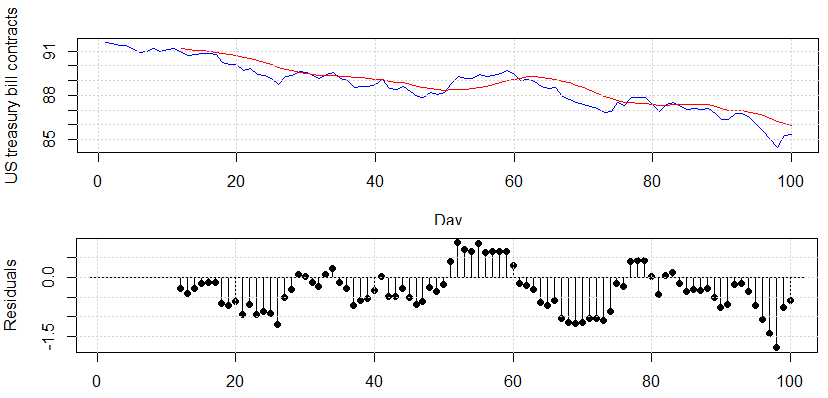
\includegraphics[width=0.92\textwidth]{biased.png}	
			\end{center}			
		\end{itemize}			
	}
	
	\only<2>{
%%%%%%%%%%%%%%%%%%%%%%%%%%%%%%%%%%%%%%%%%%%%%%%%%%%%%%%%%%%%%%%%%%%%%%%			
% Ряд перед вами спрогнозирован наивным методом - "завтра будет то же, что сегодня". Для рядов с выраженной сезонностью такой метод прогнозирования даёт не самые лучшие результаты: как видно на ACF, остатки оказываются автокоррелированными, то есть, в них остаётся ещё какая-то структура, которую можно попытаться учесть при прогнозировании.
% Автокоррелированность остатков — признак того, что в данных присутствует информация, которая не вошла в модель. Если в остатках есть структура, то можно попытаться её внести в модель явным образом. Скорректированная модель будет лучше, а её остатки будут больше похожи на белый шум. Однако это можно сделать далеко не всегда — возможности моделей не безграничны, и с их помощью иногда нельзя учесть всю структуру ряда. Таким образом, автокоррелированность остатков только указывает на потенциальную возможность улучшить модель, и не факт, что улучшения можно добиться на практике с помощью рассматриваемого класса моделей.
%%%%%%%%%%%%%%%%%%%%%%%%%%%%%%%%%%%%%%%%%%%%%%%%%%%%%%%%%%%%%%%%%%%%%%%			
		\begin{itemize}
			\item Неавтокоррелированность~--- отсутствие неучтённой зависимости от~предыдущих наблюдений:
			\begin{center}
				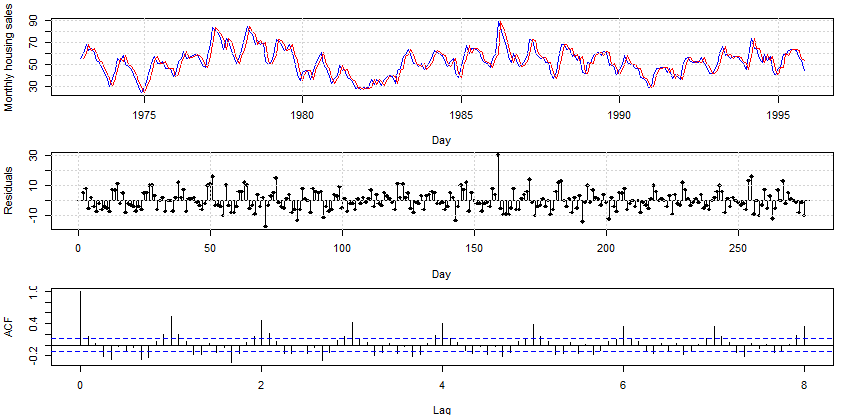
\includegraphics[width=0.92\textwidth]{autocorrelated.png}			
			\end{center}	
		\end{itemize}
	}	
    \end{frame}

    
\begin{frame}{Q-критерий Льюнга"--~Бокса}{}
	Проверим гипотезу о том, что автокорреляция равна нулю сразу при всех лагах от 1 до $L$
%%%%%%%%%%%%%%%%%%%%%%%%%%%%%%%%%%%%%%%%%%%%%%%%%%%%%%%%%%%%%%%%%%%%%%%			
% Критерий Льюнга-Бокса позволяет проверить гипотезу о том, что автокорреляция равна нулю сразу при всех лагах от 1 до L. Статистика представляет собой взвешенную сумму выборочных автокорреляций.
%%%%%%%%%%%%%%%%%%%%%%%%%%%%%%%%%%%%%%%%%%%%%%%%%%%%%%%%%%%%%%%%%%%%%%%	
	\begin{center}
		\begin{tabular}{rl}
			ряд ошибок прогноза:            & $\varepsilon^T = \varepsilon_1,\dots,\varepsilon_T;$ \\
			нулевая гипотеза:               & $H_0\colon r_1 = \dots = r_L=0;$ \\
			альтернатива:                   & $H_1\colon H_0$ неверна;\\
			статистика:                     & $Q\left(\varepsilon^T\right) = T\left(T+2\right) \sum\limits_{\tau=1}^L \frac{r_{\tau}^2}{T-\tau};$ \\
			нулевое распределение:          & $\chi^2_{L-K}$, $K$~--- число настраиваемых\\
			& параметров модели ряда.
		\end{tabular}
		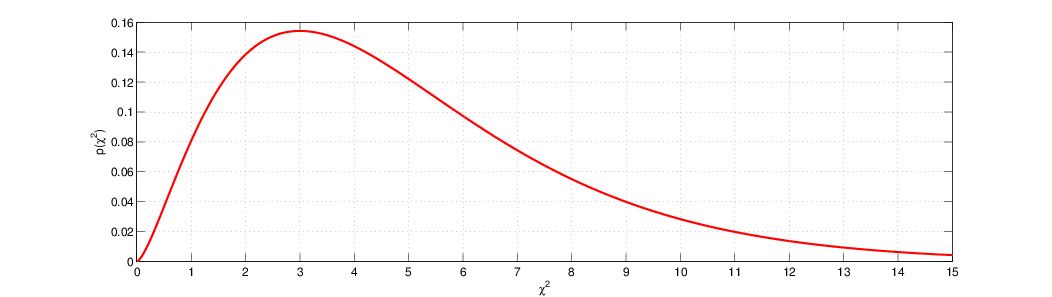
\includegraphics[width=0.8\textwidth]{chi2.png}
	\end{center}
\end{frame}
    
\begin{frame}{Отсутствие зависимости от времени}
Ряд $y_1,\dots,y_T$ \textbf{стационарен}, если $\forall s$ распределение $y_t,\dots,y_{t+s}$ не зависит от $t$, т.\,е. его свойства не зависят от времени.
%%%%%%%%%%%%%%%%%%%%%%%%%%%%%%%%%%%%%%%%%%%%%%%%%%%%%%%%%%%%%%%%%%%%%%%			
% Если остатки смещены, это значит, что пронозы станут в среднем лучше, если добавить к ним константу, на которую проиходит смещение. Ряд перед вами мы попробовали спрогнозировать наивным сезонным методом, когда в качестве прогноза выбирается значение ряда в предыдущий такой же сезон. Такой прогноз оказывается смещённым, поэтому мы его корректируем на константу. Однако, это делает остатки нестационарными: несмотря на то, что в среднем по периоду смещения нет, прогнозные значения в начале периода оказываются заниженными, в конце - завышенными.
%%%%%%%%%%%%%%%%%%%%%%%%%%%%%%%%%%%%%%%%%%%%%%%%%%%%%%%%%%%%%%%%%%%%%%%			
		\begin{itemize}
			\item Стационарность~--- отсутствие зависимости от времени:
			\begin{center}
				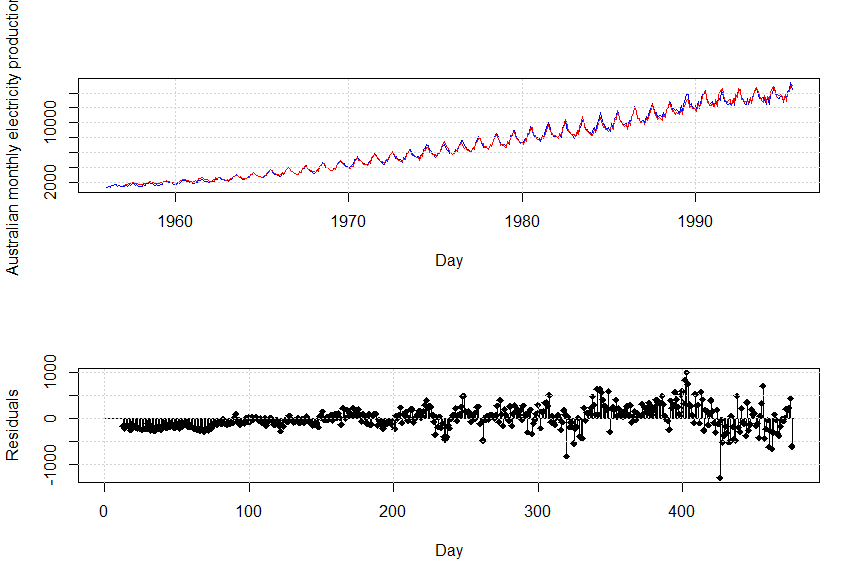
\includegraphics[width=0.6\textwidth]{trended.png}			
			\end{center}		
		\end{itemize}		
		
\end{frame}

\begin{frame}{Критерий KPSS (Kwiatkowski-Philips-Schmidt-Shin)}
%%%%%%%%%%%%%%%%%%%%%%%%%%%%%%%%%%%%%%%%%%%%%%%%%%%%%%%%%%%%%%%%%%%%%%%			
% Формально гипотезу о стационарности можно проверить с помощью критерия KPSS. Статистика критерия выглядит достаточно сложно, не будем вдаваться в подробности. Вообще говоря, существует большое количество критериев для проверки гипотезы о стационарности, на практике можно использовать любой из них. Следите только, что именно для критерия является нулевой гипотезой - у некоторых критериев это стационарность, как у KPSS, у других, наоборот, её отсутствие.
%%%%%%%%%%%%%%%%%%%%%%%%%%%%%%%%%%%%%%%%%%%%%%%%%%%%%%%%%%%%%%%%%%%%%%%			
	\begin{center}
		\begin{tabular}{rl}
			ряд ошибок прогноза:            & $\varepsilon^T = \varepsilon_1,\dots,\varepsilon_T;$ \\
			нулевая гипотеза:               & $H_0\colon$ ряд $\varepsilon^T$ стационарен;\\
			альтернатива:                   & $H_1\colon$ ряд $\varepsilon^T$ описывается моделью \\
			& вида $\varepsilon_t = \alpha\varepsilon_{t-1};$ \\
			статистика:                     & $KPSS\left(\varepsilon^T\right) = \frac1{T^2} \sum\limits_{i=1}^T \left(\sum\limits_{t=1}^i \varepsilon_t\right)^2 \Big/ \lambda^2,$ \\
            &$\lambda^2$---оценка дисперсии ошибок;\\
			нулевое распределение:          & табличное.\\
		\end{tabular}
	\end{center}
	
	\bigskip
	
	Есть и другие критерии для проверки стационарности: Дики"=Фуллера, Филлипса"=Перрона и их многочисленные модификации\footnote{Patterson K.  \textit{Unit root tests in time series, volume 1: key concepts and problems}. --- Palgrave Macmillan, 2011}
\end{frame}


\begin{frame}{Как проверить свойства остатков прогноза?}
		\begin{itemize}
		\item Несмещённость~--- критерий Стьюдента или Уилкоксона
		\item Неавтокоррелированность~--- коррелограмма, Q-критерий Льюнга"--~Бокса.
		\item Стационарность~--- визуальный анализ, критерий KPSS.
		\item Нормальность --- q-q plot, критерий Шапиро"--~Уилка
			% \begin{center}
			% 	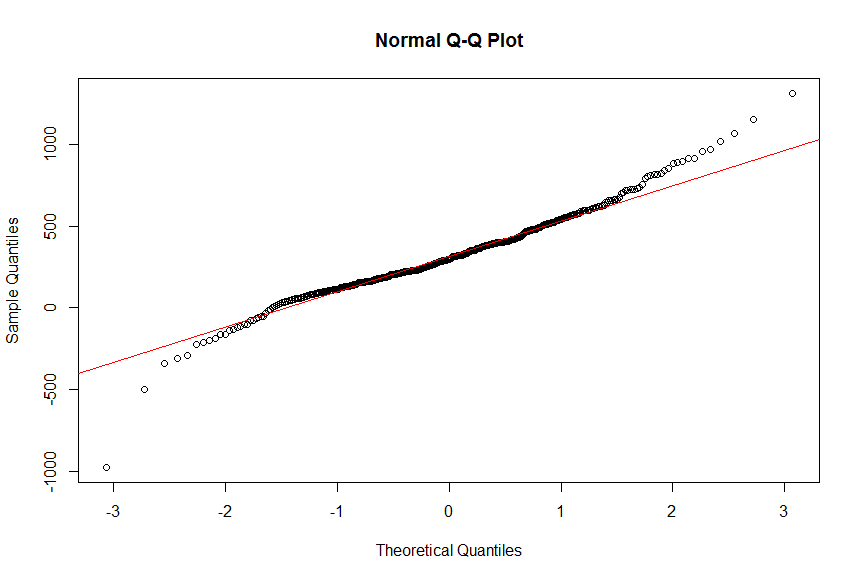
\includegraphics[width=0.6\textwidth]{qqplot.png}			
			% \end{center}		
	\end{itemize}
\end{frame}






%%%%%%%%%%%%%%%%%%%%%%%%%%%%%%%%%%%%%%%%%%%

\end{document}

\subsection{Стационарность}
\begin{frame}{Стационарность}
	\only<1>{
%%%%%%%%%%%%%%%%%%%%%%%%%%%%%%%%%%%%%%%%%%%%%%%%%%%%%%%%%%%%%%%%%%%%%%%	
% Важное свойство временных рядов — это стационарность. Временной ряд  называется стационарным, если распределение его отсчётов в окне произвольной фиксированной ширины не зависит от положения этого окна, т.е. свойства ряда не зависят от времени.
% Из этого определения следует, что ряды, в которых присутствует тренд, являются нестационарными: в зависимости от расположения окна изменяется средний уровень ряда. Кроме того, нестационарны ряды с сезонностью: если ширина окна меньше сезонного периода, то распределение ряда будет разным в зависимости от положения окна. При этом интересно, что ряды, в которых есть непериодические циклы, не обязательно являются нестационарными, поскольку нельзя заранее предсказать положение максимумов и минимумов этого ряда.
%%%%%%%%%%%%%%%%%%%%%%%%%%%%%%%%%%%%%%%%%%%%%%%%%%%%%%%%%%%%%%%%%%%%%%%	
		Ряд $y_1,\dots,y_T$ \textbf{стационарен}, если $\forall s$ распределение $y_t,\dots,y_{t+s}$ не зависит от $t$, т.\,е. его свойства не зависят от времени.
		
		\bigskip
		
		Ряды с трендом или сезонностью нестационарны.
		
		\bigskip
		
		Ряды с непериодическими циклами стационарны, поскольку нельзя предсказать заранее, где будут находится максимумы и~минимумы.
	}
	
	\only<2>{
%%%%%%%%%%%%%%%%%%%%%%%%%%%%%%%%%%%%%%%%%%%%%%%%%%%%%%%%%%%%%%%%%%%%%%%	
% Как вы думаете, какие из этих рядов стационарны?
%%%%%%%%%%%%%%%%%%%%%%%%%%%%%%%%%%%%%%%%%%%%%%%%%%%%%%%%%%%%%%%%%%%%%%%	
		\begin{center}
			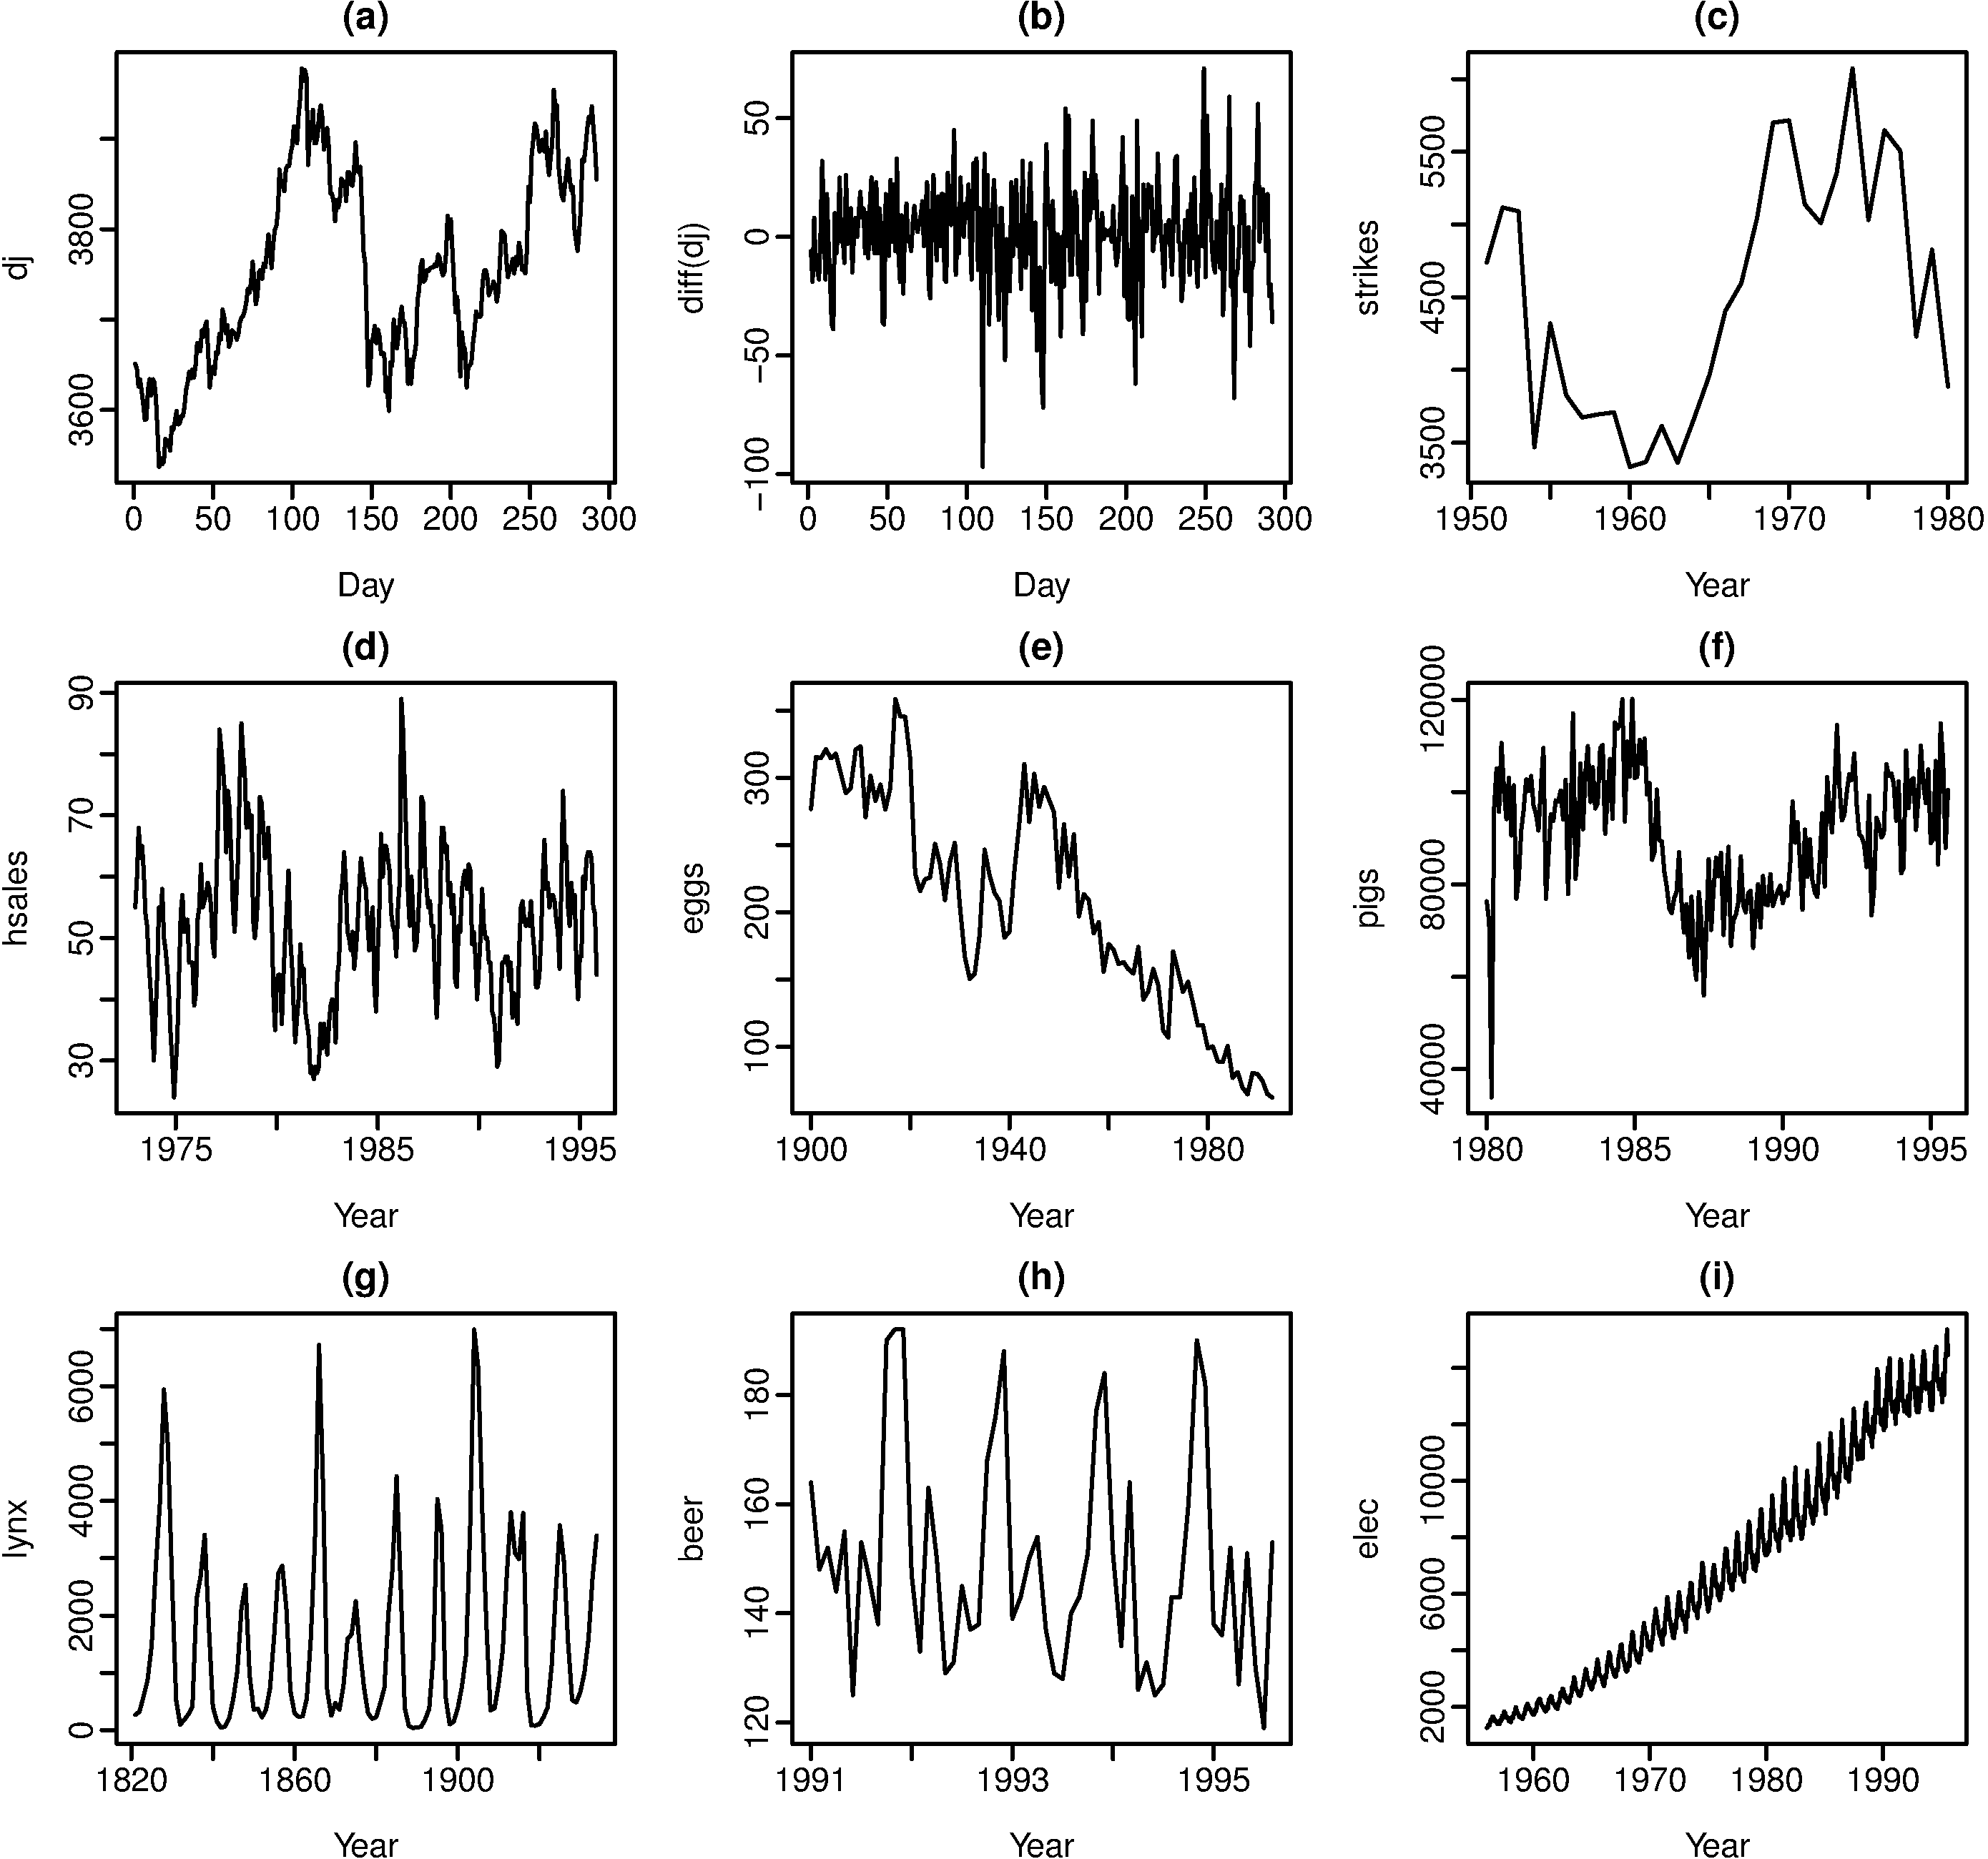
\includegraphics[height=0.7\textheight]{stationary.png}			
		\end{center}	
	}
	
	\only<3>{
		Нестационарны из-за сезонности:
		\begin{center}
			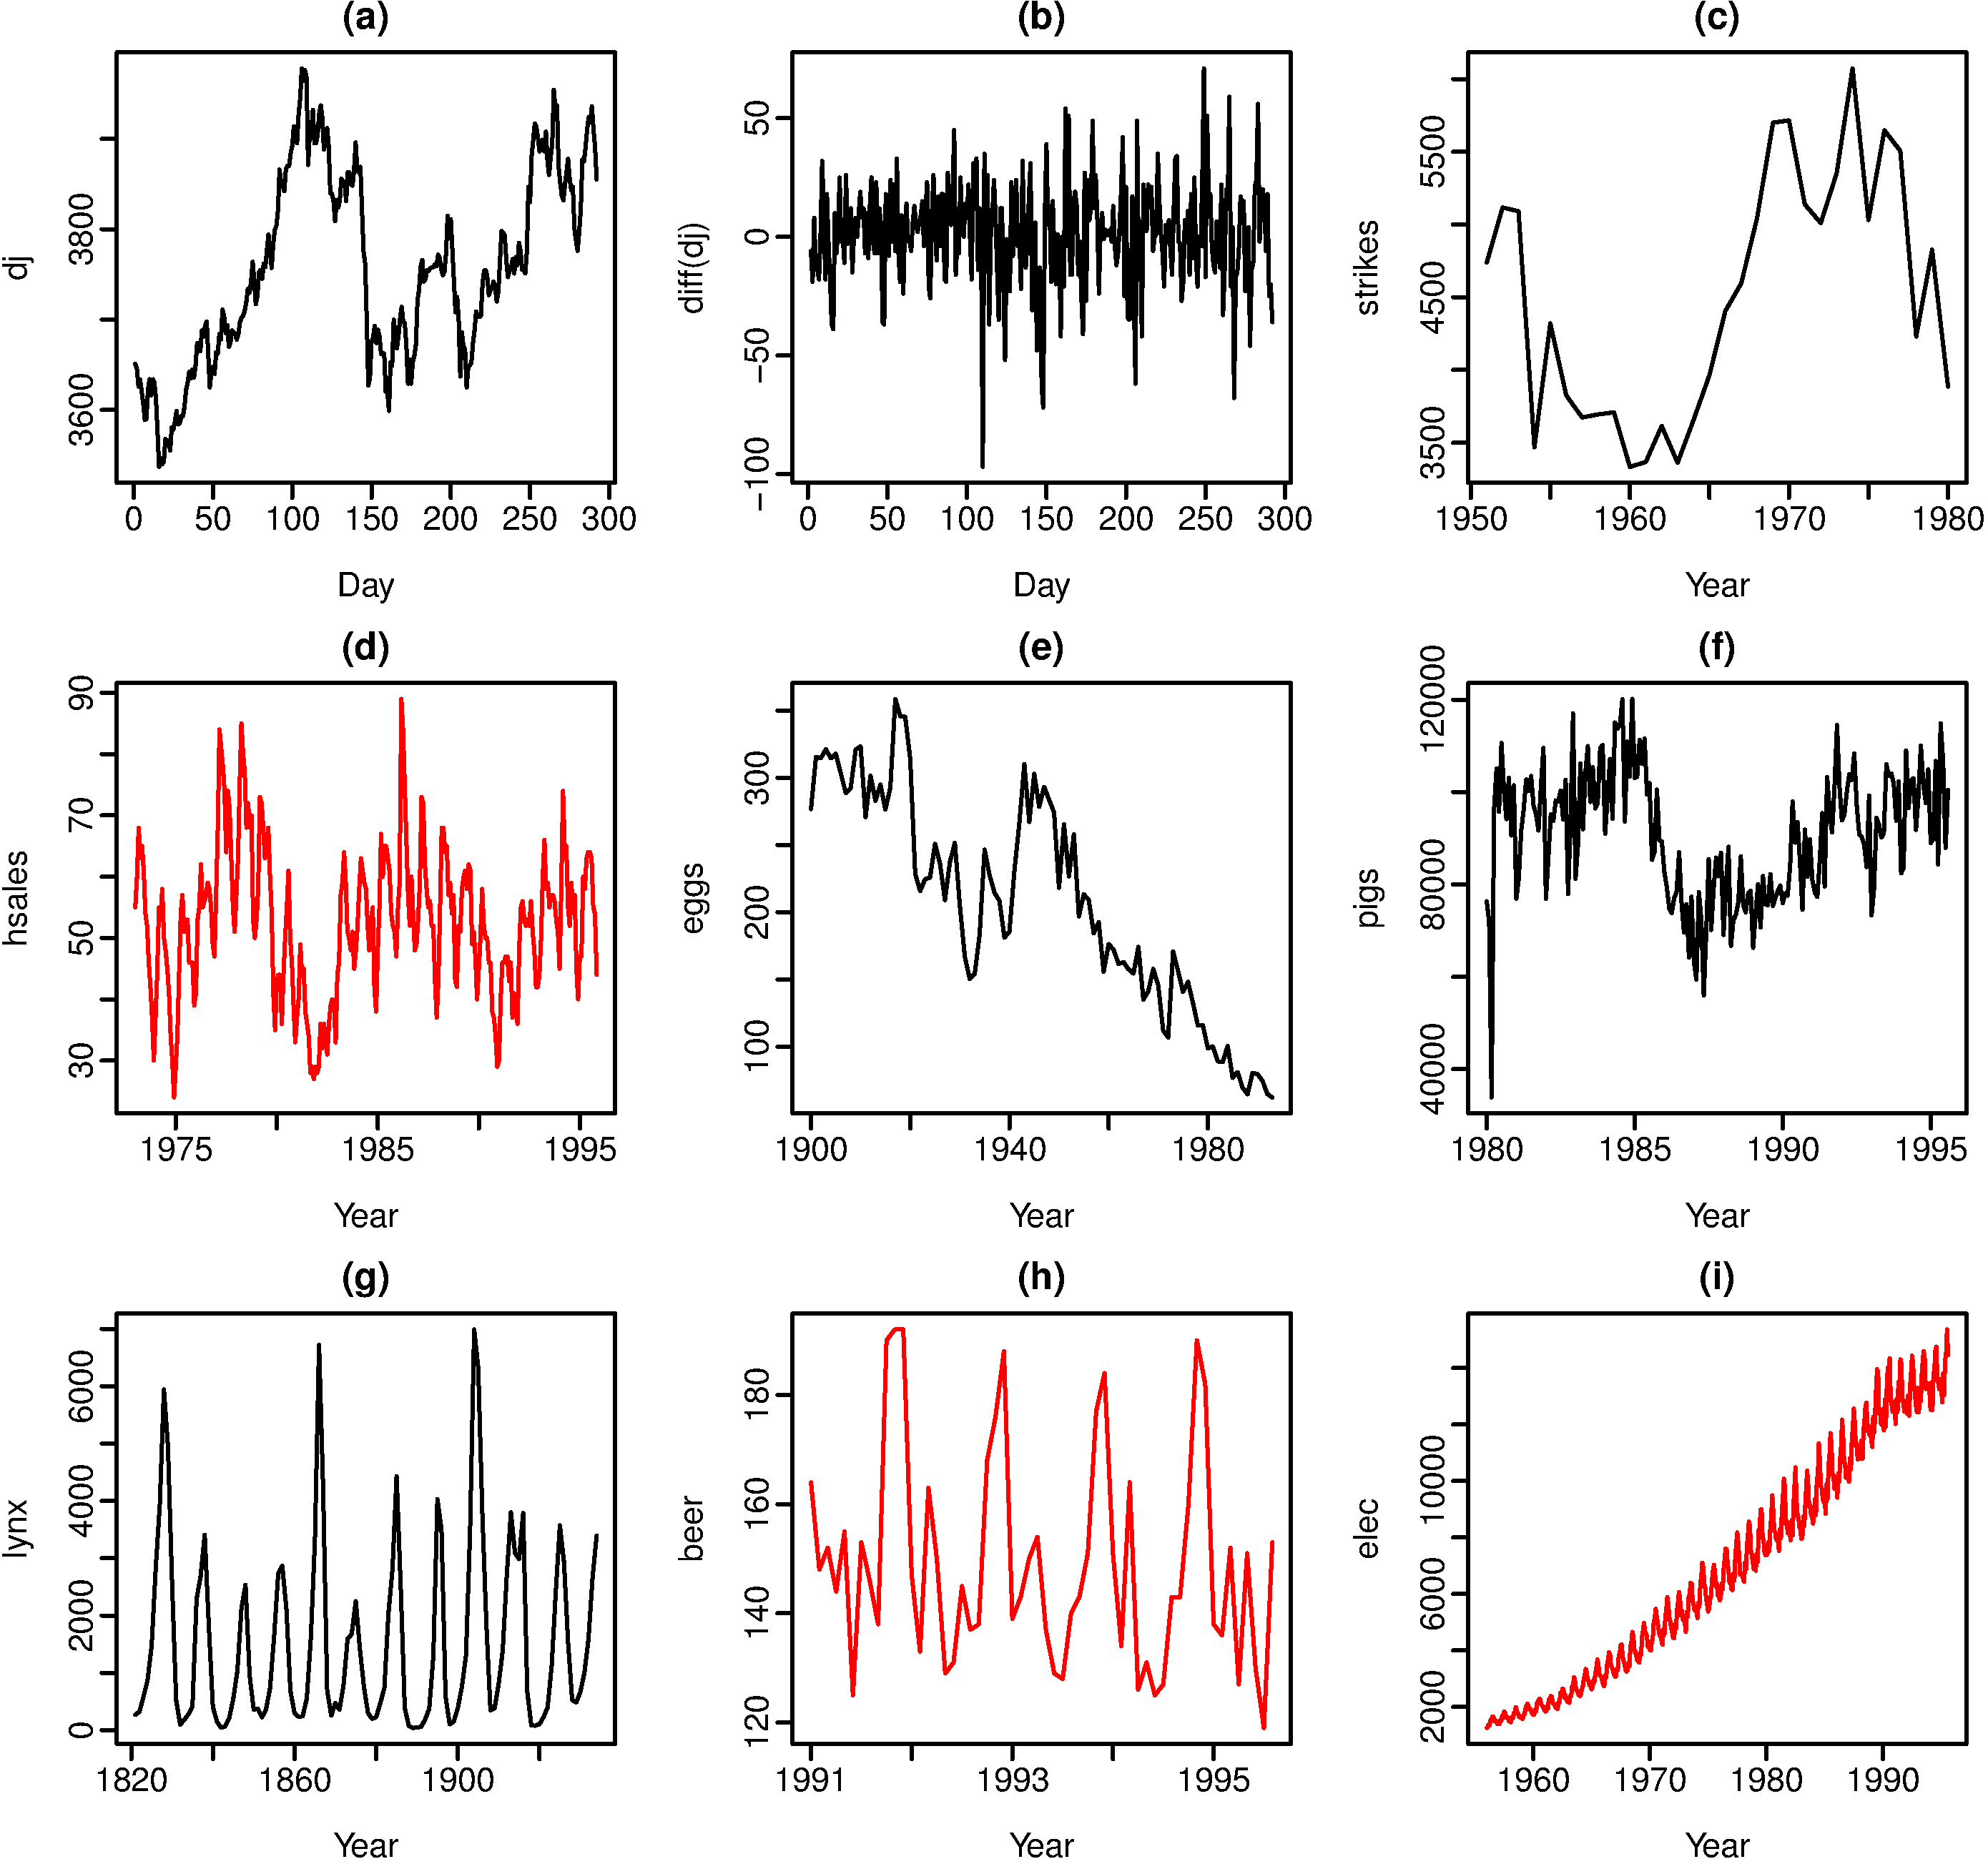
\includegraphics[height=0.7\textheight]{stationary1.png}			
		\end{center}	
	}	
	
	\only<4>{
		Нестационарны из-за тренда:
		\begin{center}
			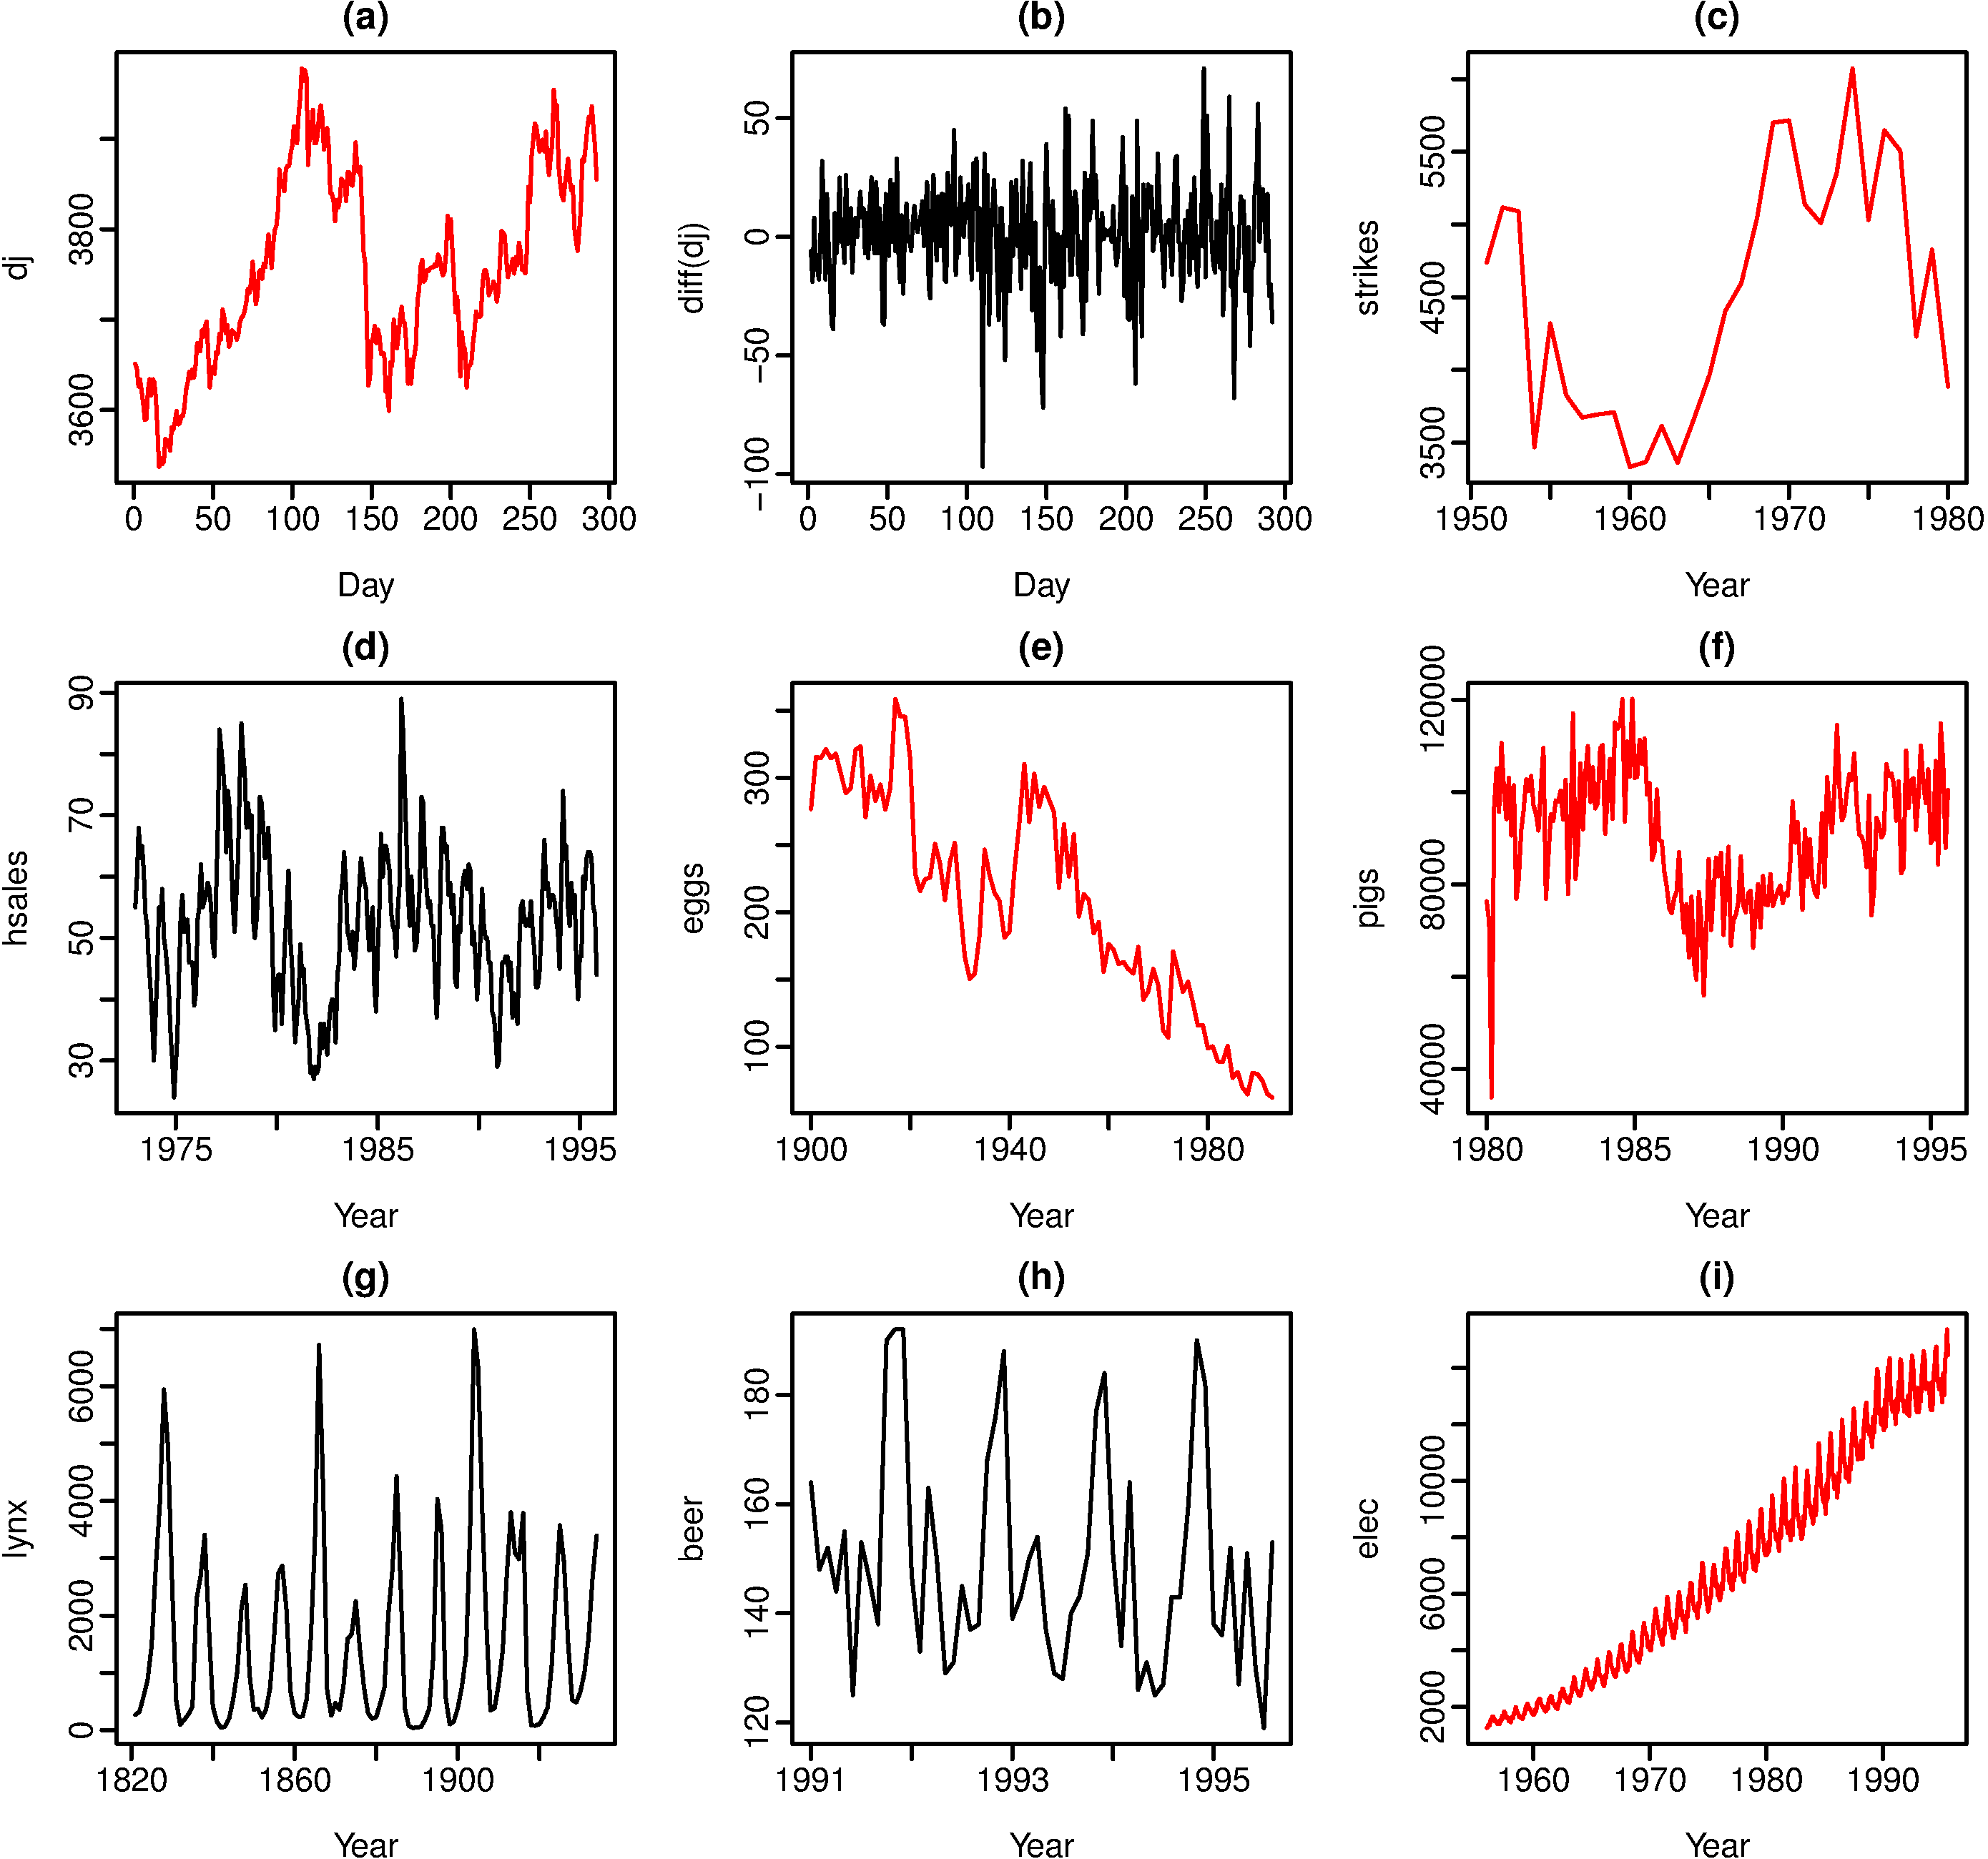
\includegraphics[height=0.7\textheight]{stationary2.png}			
		\end{center}	
	}		
	
	\only<5>{
		Нестационарны из-за меняющейся дисперсии:
		\begin{center}
			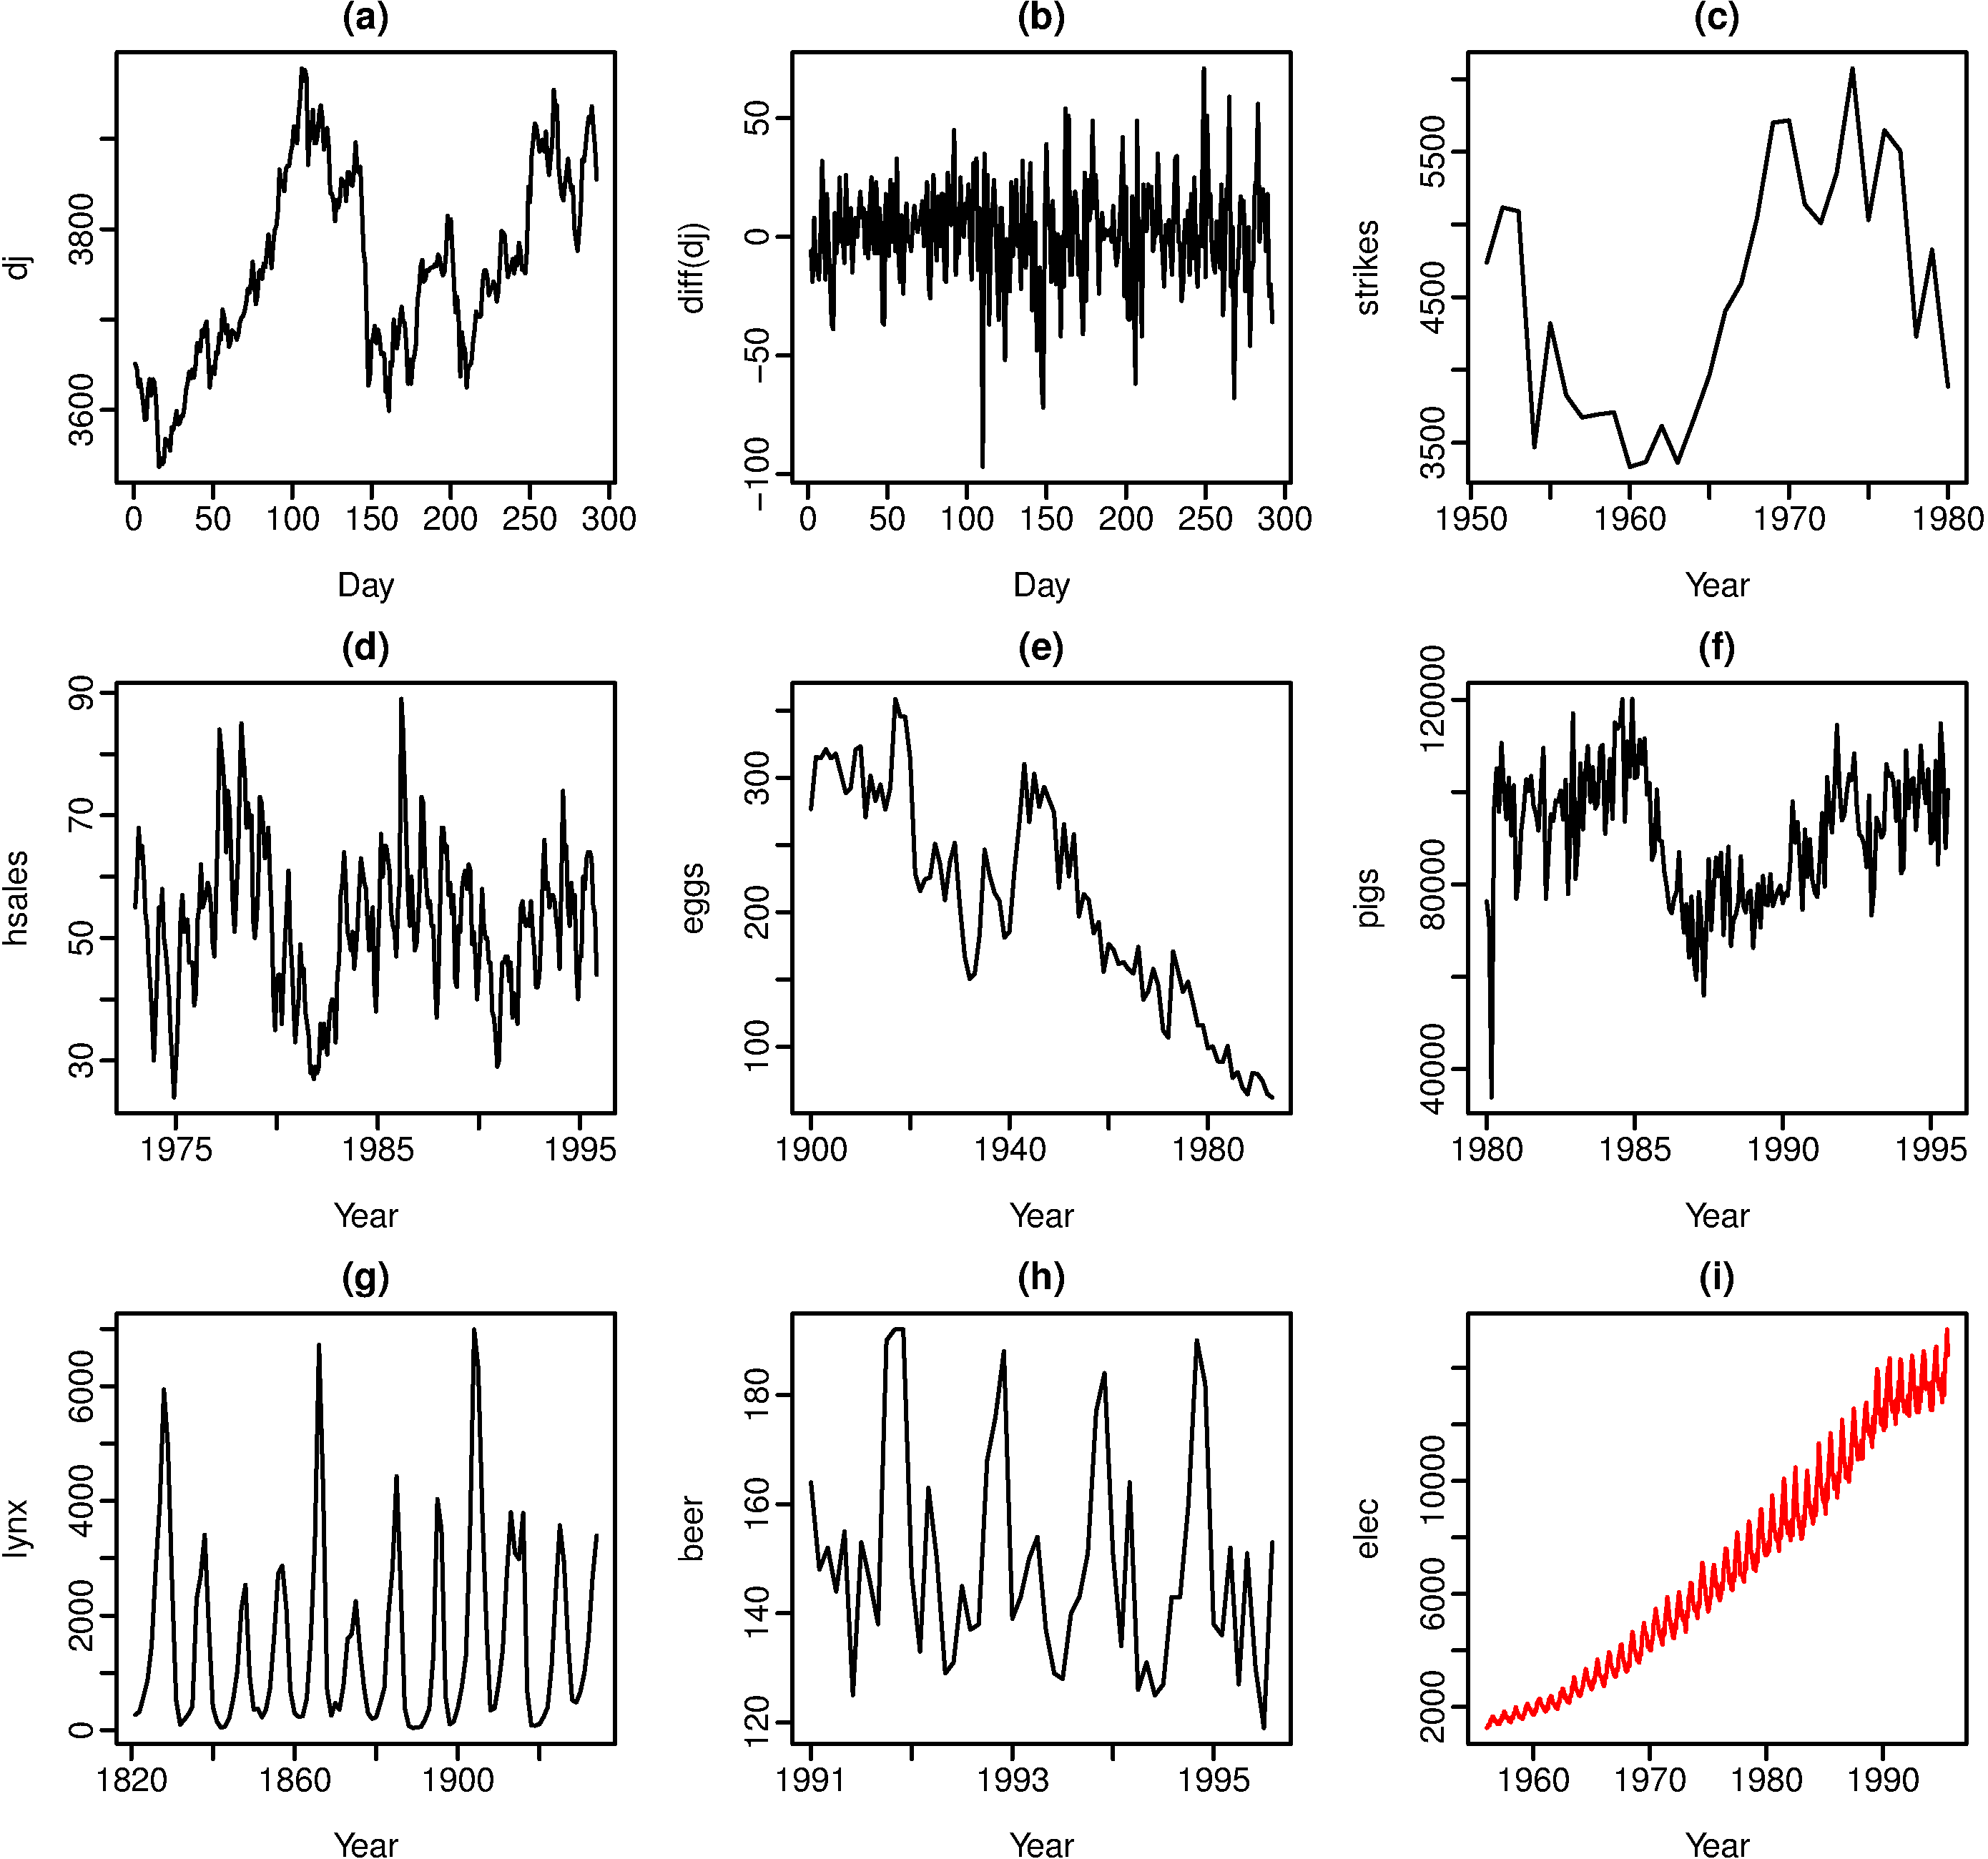
\includegraphics[height=0.7\textheight]{stationary3.png}			
		\end{center}	
	}
	
	\only<6>{
		Стационарны:
		\begin{center}
			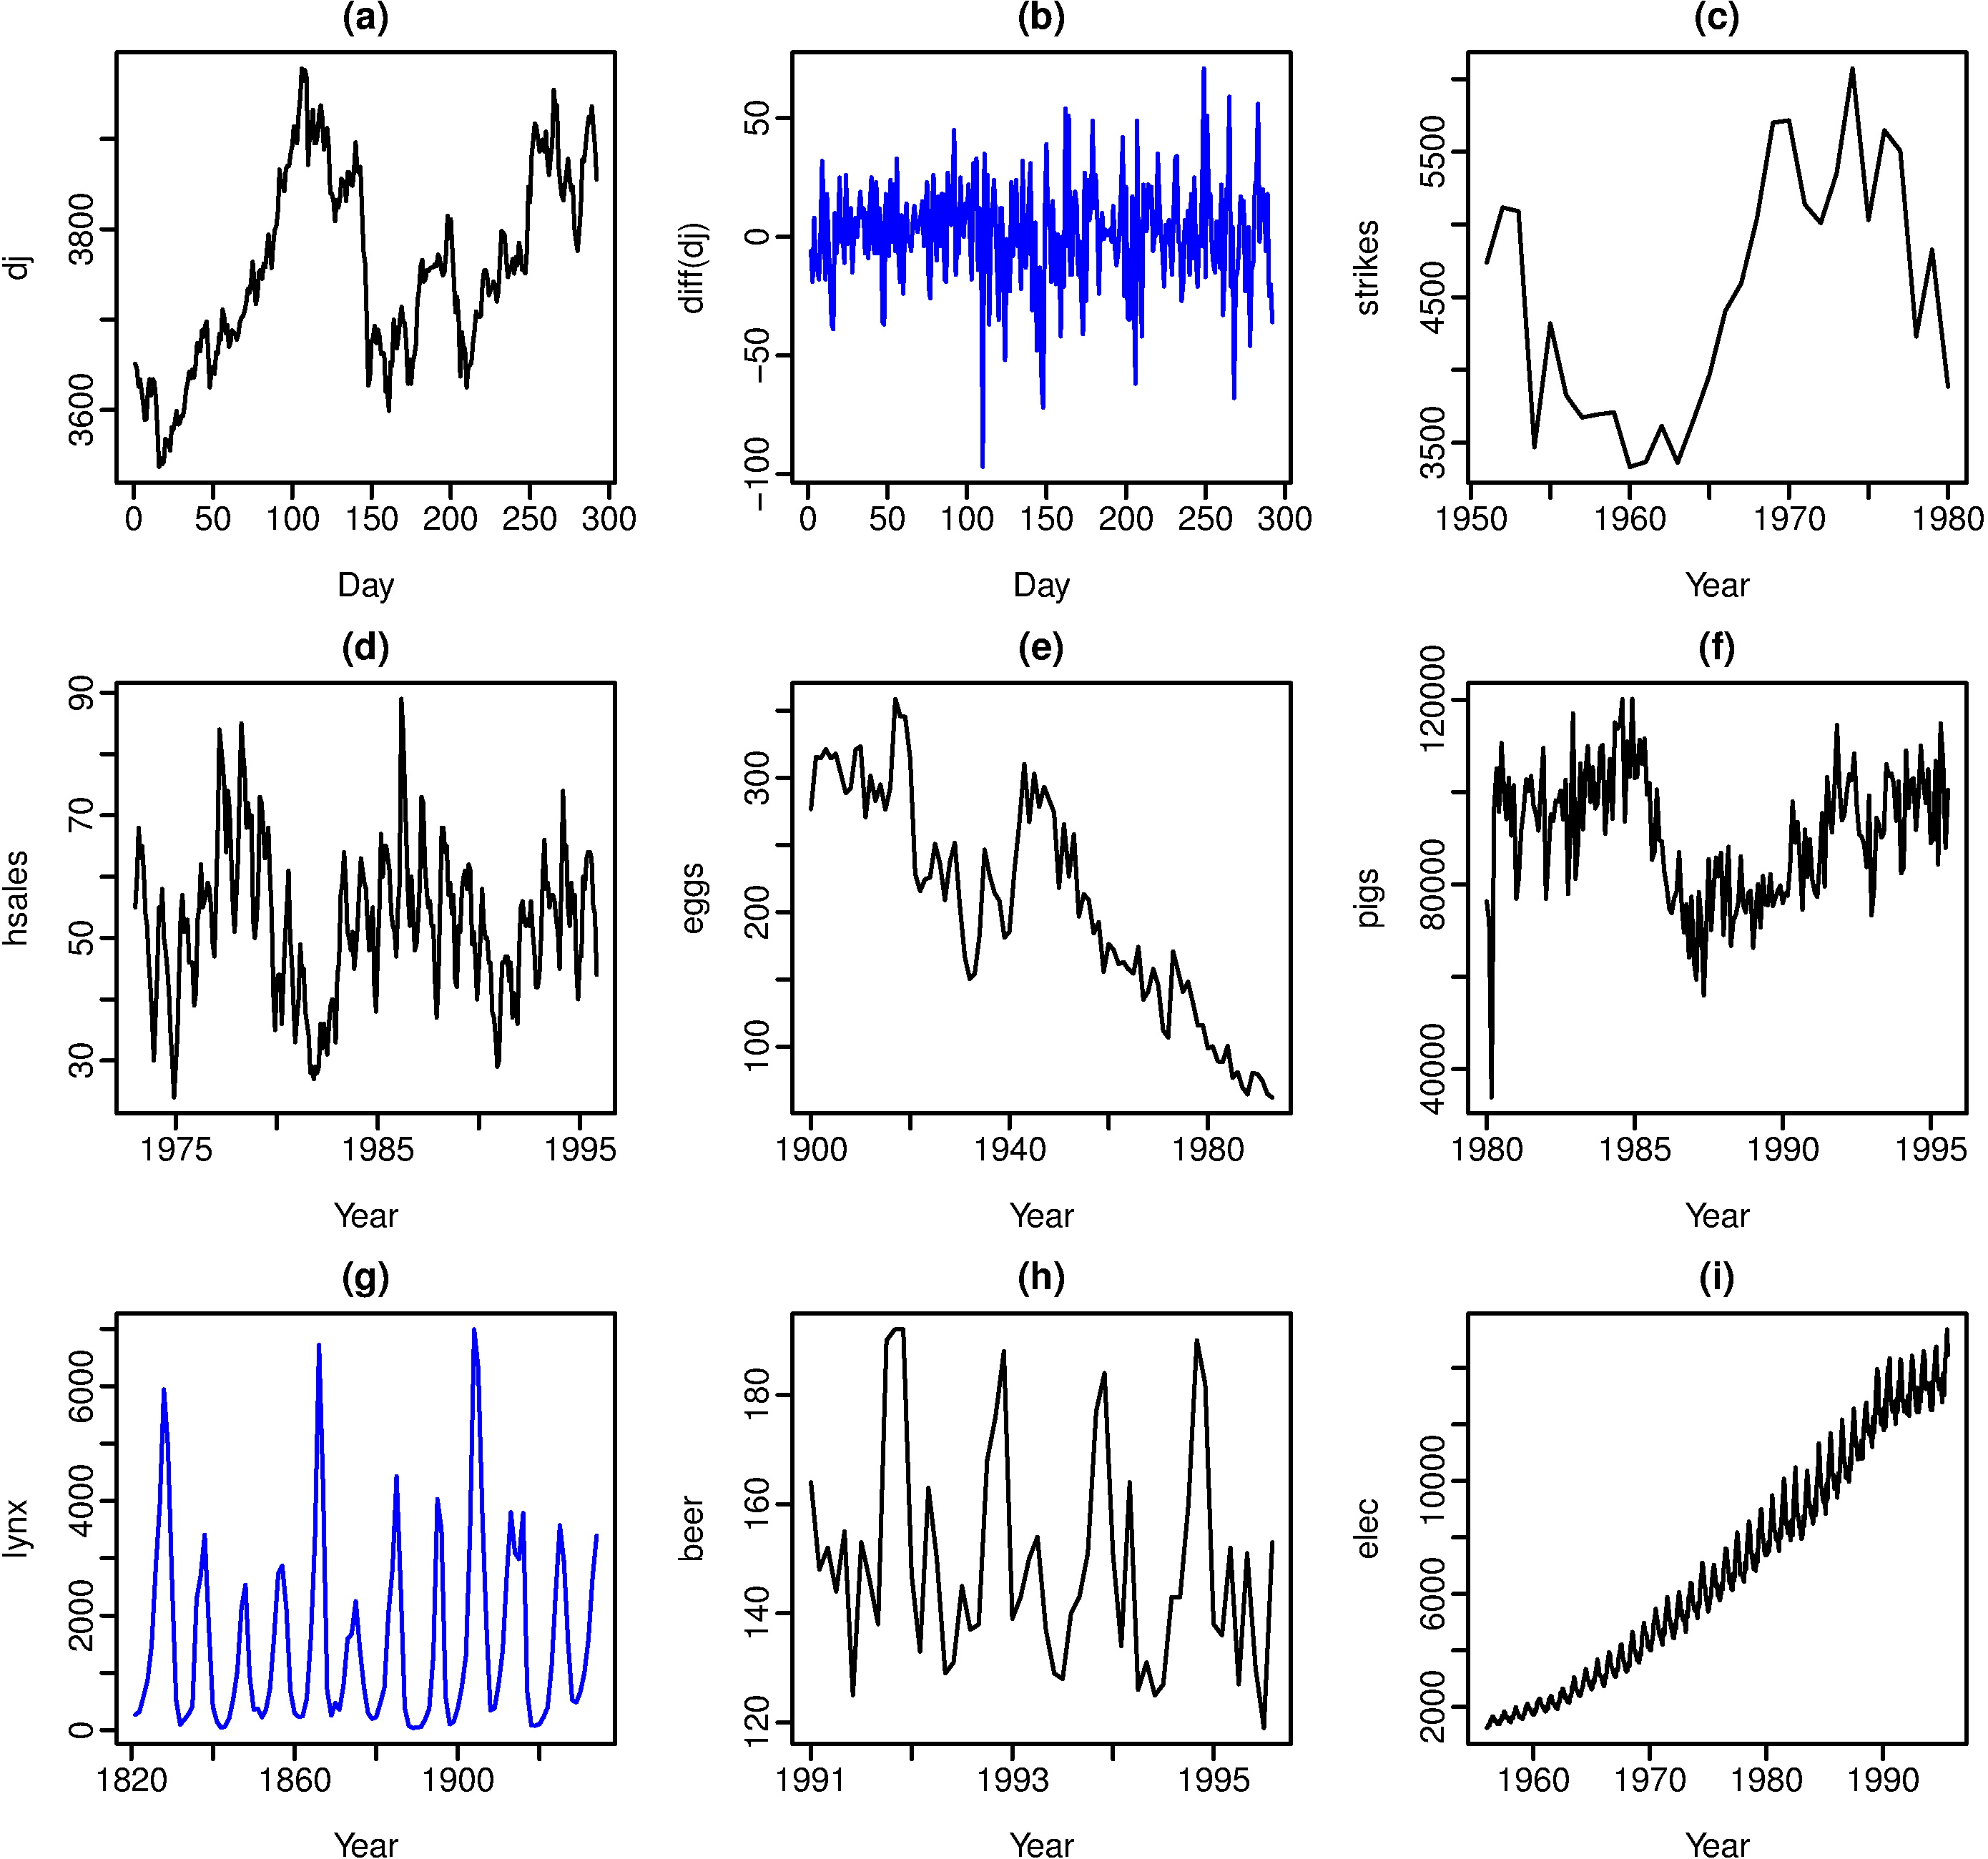
\includegraphics[height=0.7\textheight]{stationary4.png}
		\end{center}	
	}
\end{frame}


\begin{frame}{Критерий KPSS (Kwiatkowski-Philips-Schmidt-Shin)}
%%%%%%%%%%%%%%%%%%%%%%%%%%%%%%%%%%%%%%%%%%%%%%%%%%%%%%%%%%%%%%%%%%%%%%%			
% Формально гипотезу о стационарности можно проверить с помощью критерия KPSS. Статистика критерия выглядит достаточно сложно, не будем вдаваться в подробности. Вообще говоря, существует большое количество критериев для проверки гипотезы о стационарности, на практике можно использовать любой из них. Следите только, что именно для критерия является нулевой гипотезой - у некоторых критериев это стационарность, как у KPSS, у других, наоборот, её отсутствие.
%%%%%%%%%%%%%%%%%%%%%%%%%%%%%%%%%%%%%%%%%%%%%%%%%%%%%%%%%%%%%%%%%%%%%%%			
	\begin{center}
		\begin{tabular}{rl}
			ряд ошибок прогноза:            & $\varepsilon^T = \varepsilon_1,\dots,\varepsilon_T;$ \\
			нулевая гипотеза:               & $H_0\colon$ ряд $\varepsilon^T$ стационарен;\\
			альтернатива:                   & $H_1\colon$ ряд $\varepsilon^T$ описывается моделью \\
			& вида $\varepsilon_t = \alpha\varepsilon_{t-1};$ \\
			статистика:                     & $KPSS\left(\varepsilon^T\right) = \frac1{T^2} \sum\limits_{i=1}^T \left(\sum\limits_{t=1}^i \varepsilon_t\right)^2 \Big/ \lambda^2,$ \\
            &$\lambda^2$---оценка дисперсии ошибок;\\
			нулевое распределение:          & табличное.\\
		\end{tabular}
	\end{center}
	
	\bigskip
	
	Другие критерии для проверки стационарности: Дики"=Фуллера, Филлипса"=Перрона и их многочисленные модификации (см. Patterson K.  \textit{Unit root tests in time series, volume 1: key concepts and problems}. --- Palgrave Macmillan, 2011).	
\end{frame}


\subsection{Преобразования ряда}
\begin{frame}{Стабилизация дисперсии}
%%%%%%%%%%%%%%%%%%%%%%%%%%%%%%%%%%%%%%%%%%%%%%%%%%%%%%%%%%%%%%%%%%%%%%%	
% При работе с нестационарными временными рядами используется ряд стандартных трюков, чтобы сделать их стационарными. В случае, если во временном ряде монотонно по времени изменяется дисперсия, применяется специальное преобразование, стабилизирующее дисперсию. Очень часто в качестве такого преобразования выступает логарифмирование. Результат стабилизации дисперсии для ряда производства электричества в Австралии показан на рисунке 1.15. Видно, что после логарифмирования размах колебаний в начале и конце ряда становится очень похожим, и дисперсия примерно стабилизируется.
%%%%%%%%%%%%%%%%%%%%%%%%%%%%%%%%%%%%%%%%%%%%%%%%%%%%%%%%%%%%%%%%%%%%%%%	
	Для рядов с монотонно меняющейся дисперсией можно использовать стабилизирующие преобразования.
	
	
	\bigskip
	
	Часто используют логарифмирование:
	
	\bigskip
	
	\begin{center}
		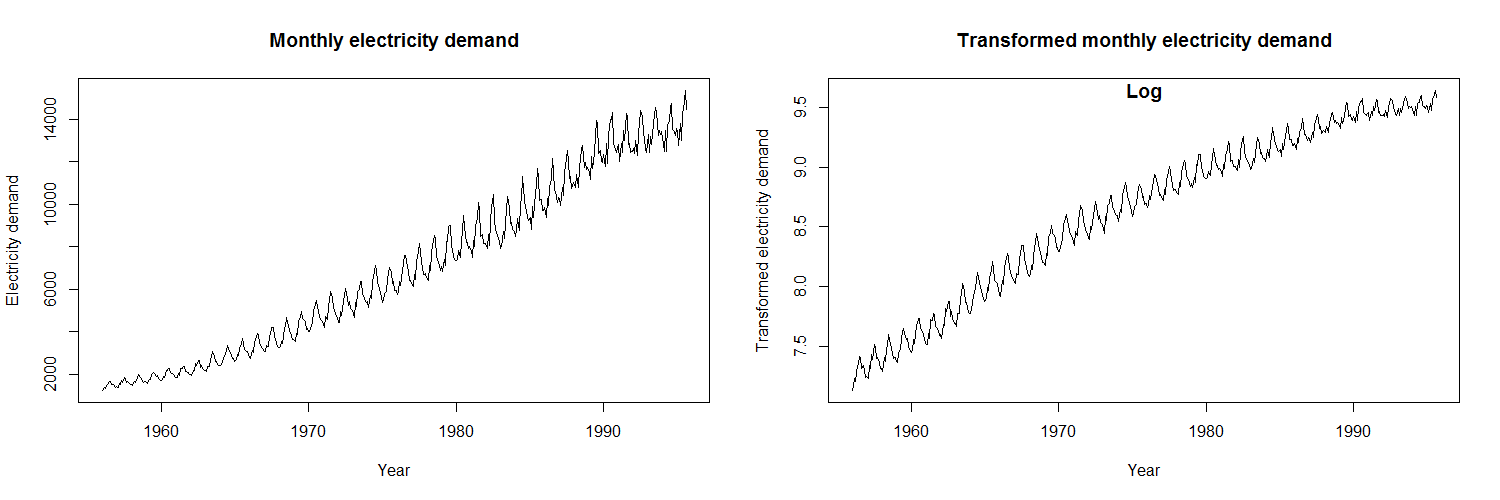
\includegraphics[width=0.8\textwidth]{logtrans.png}
	\end{center}		
\end{frame}

\begin{frame}{Преобразования Бокса-Кокса}	
	\only<1>{
%%%%%%%%%%%%%%%%%%%%%%%%%%%%%%%%%%%%%%%%%%%%%%%%%%%%%%%%%%%%%%%%%%%%%%%	
% Логарифмирование принадлежит к семейству преобразований Бокса-Кокса. Это параметрическое семейство функций, в котором параметр  определяет, как именно будет преобразован ряд: лямбда = 0 — это логарифмирование, лямбда = 1 — тождественное преобразование ряда, а при других значениях лямбда — степенное преобразование. Значение параметра можно подбирать так, чтобы дисперсия была как можно более стабильной во времени. Так, для ряда по данным производства электричества в Австралии оптимальное значение  = 0:27, при этом дисперсия немного более стабильна, чем при логарифмировании.
%%%%%%%%%%%%%%%%%%%%%%%%%%%%%%%%%%%%%%%%%%%%%%%%%%%%%%%%%%%%%%%%%%%%%%%	
		Параметрическое семейство стабилизирующих дисперсию преобразований:	
		$$
		y'_t=\begin{cases}
		\ln y_t, & \lambda=0, \\
		\left(y_t^\lambda-1\right)/\lambda, & \lambda\neq 0.
		\end{cases}
		$$	
		
		\bigskip
		
		Параметр $\lambda$ выбирается так, чтобы минимизировать дисперсию или максимизировать правдоподобие модели.
		
		\bigskip
		
		\begin{center}
			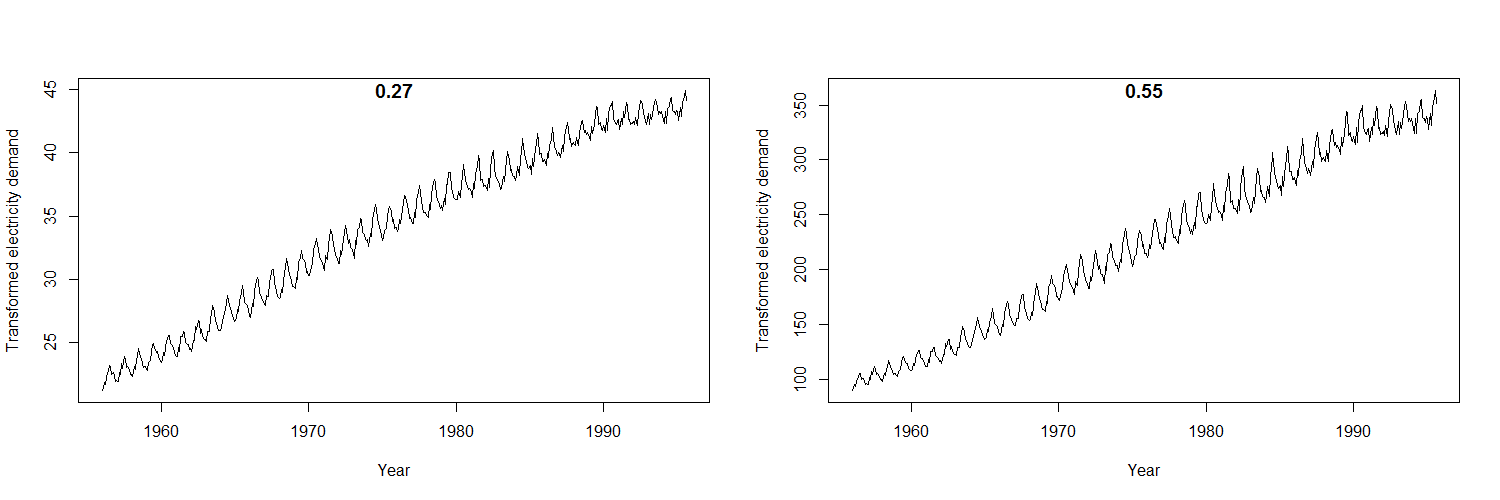
\includegraphics[width=0.8\textwidth]{boxcox.png}
		\end{center}
	}
	
	\only<2>{
		После построения прогноза для трансформированного ряда его нужно преобразовать в прогноз исходного:
		$$
		\hat{y}_t=\begin{cases}
		\exp\left(\hat{y}'_t\right), & \lambda=0, \\
		\left(\lambda\hat{y}'_t+1\right)^{1/\lambda}, & \lambda\neq 0.
		\end{cases}
		$$			
		
		\bigskip
		
		\begin{itemize}
			\item если некоторые $y_t\leq0$, преобразования Бокса-Кокса невозможны (нужно прибавить к ряду константу)
			\item часто оказывается, что преобразование вообще не нужно
			\item можно округлять значение $\lambda,$ чтобы упростить интерпретацию
			\item как правило, стабилизирующее преобразование слабо влияет на~прогноз и сильно~--- на~предсказательный интервал
		\end{itemize}
	}
\end{frame}

\begin{frame}{Дифференцирование}
	\only<1>{
%%%%%%%%%%%%%%%%%%%%%%%%%%%%%%%%%%%%%%%%%%%%%%%%%%%%%%%%%%%%%%%%%%%%%%%	
% Ещё один важный трюк, который позволяет сделать ряд стационарным, — это дифференцирование, переход к попарным разностям соседних значений. Для нестационарного ряда часто оказывается, что получаемый после дифференцирования ряд является стационарным. Такая операция позволяет стабилизировать среднее значение ряда и избавиться от тренда, а иногда даже от сезонности. Кроме того, дифференцирование можно применять неоднократно: от ряда первых разностей, продифференцировав его, можно прийти к ряду вторых разностей, и т. д. Длина ряда при этом каждый раз будет немного сокращаться, но при этом он будет стационарным.
%%%%%%%%%%%%%%%%%%%%%%%%%%%%%%%%%%%%%%%%%%%%%%%%%%%%%%%%%%%%%%%%%%%%%%%	
		\textbf{Дифференцирование ряда}~--- переход к попарным разностям его соседних значений:
		$$y_1,\dots,y_T \;\longrightarrow \;y'_2,\dots,y'_{T}, $$
		$$y'_t = y_t - y_{t-1}.$$
		
		Дифференцированием можно стабилизировать среднее значение ряда и~избавиться от тренда и сезонности.
		
		\bigskip
		
		Может применяться неоднократное дифференцирование; например, для второго порядка:
		$$y_1,\dots,y_T \longrightarrow y'_2,\dots,y'_{T} \longrightarrow y''_3,\dots,y''_{T},$$	
		$$y''_t = y'_t-y'_{t-1} = y_t - 2y_{t-1} + y_{t-2}.$$		
	}
	
	\only<2>{
		\begin{center}
			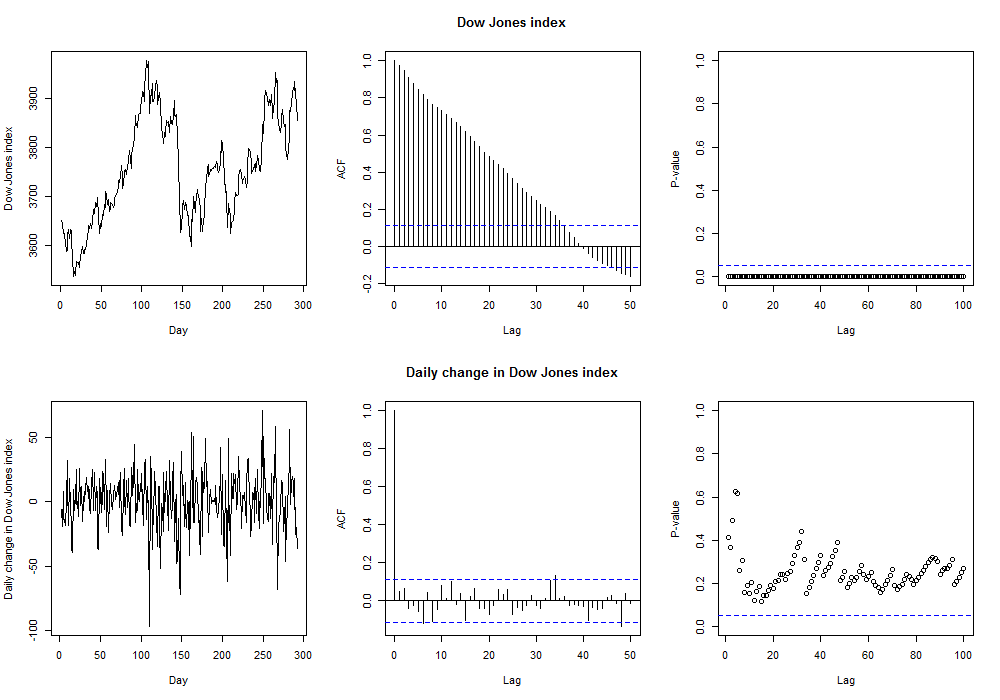
\includegraphics[height=0.8\textheight]{diff1.png}
		\end{center}	
		Критерий KPSS: для исходного ряда $p<0.01$, для ряда первых разностей~--- $p>0.1.$
	}
\end{frame}

\begin{frame}{Сезонное дифференцирование}
	\only<1>{
		\textbf{Сезонное дифференцирование ряда}~--- переход к попарным разностям его значений в соседних сезонах:
		$$y_1,\dots,y_T \;\longrightarrow \;y'_{s+1},\dots,y'_{T}, $$
		$$y'_t = y_t - y_{t-s}.$$	
	}
	
	\only<2>{

    	\begin{center}
    		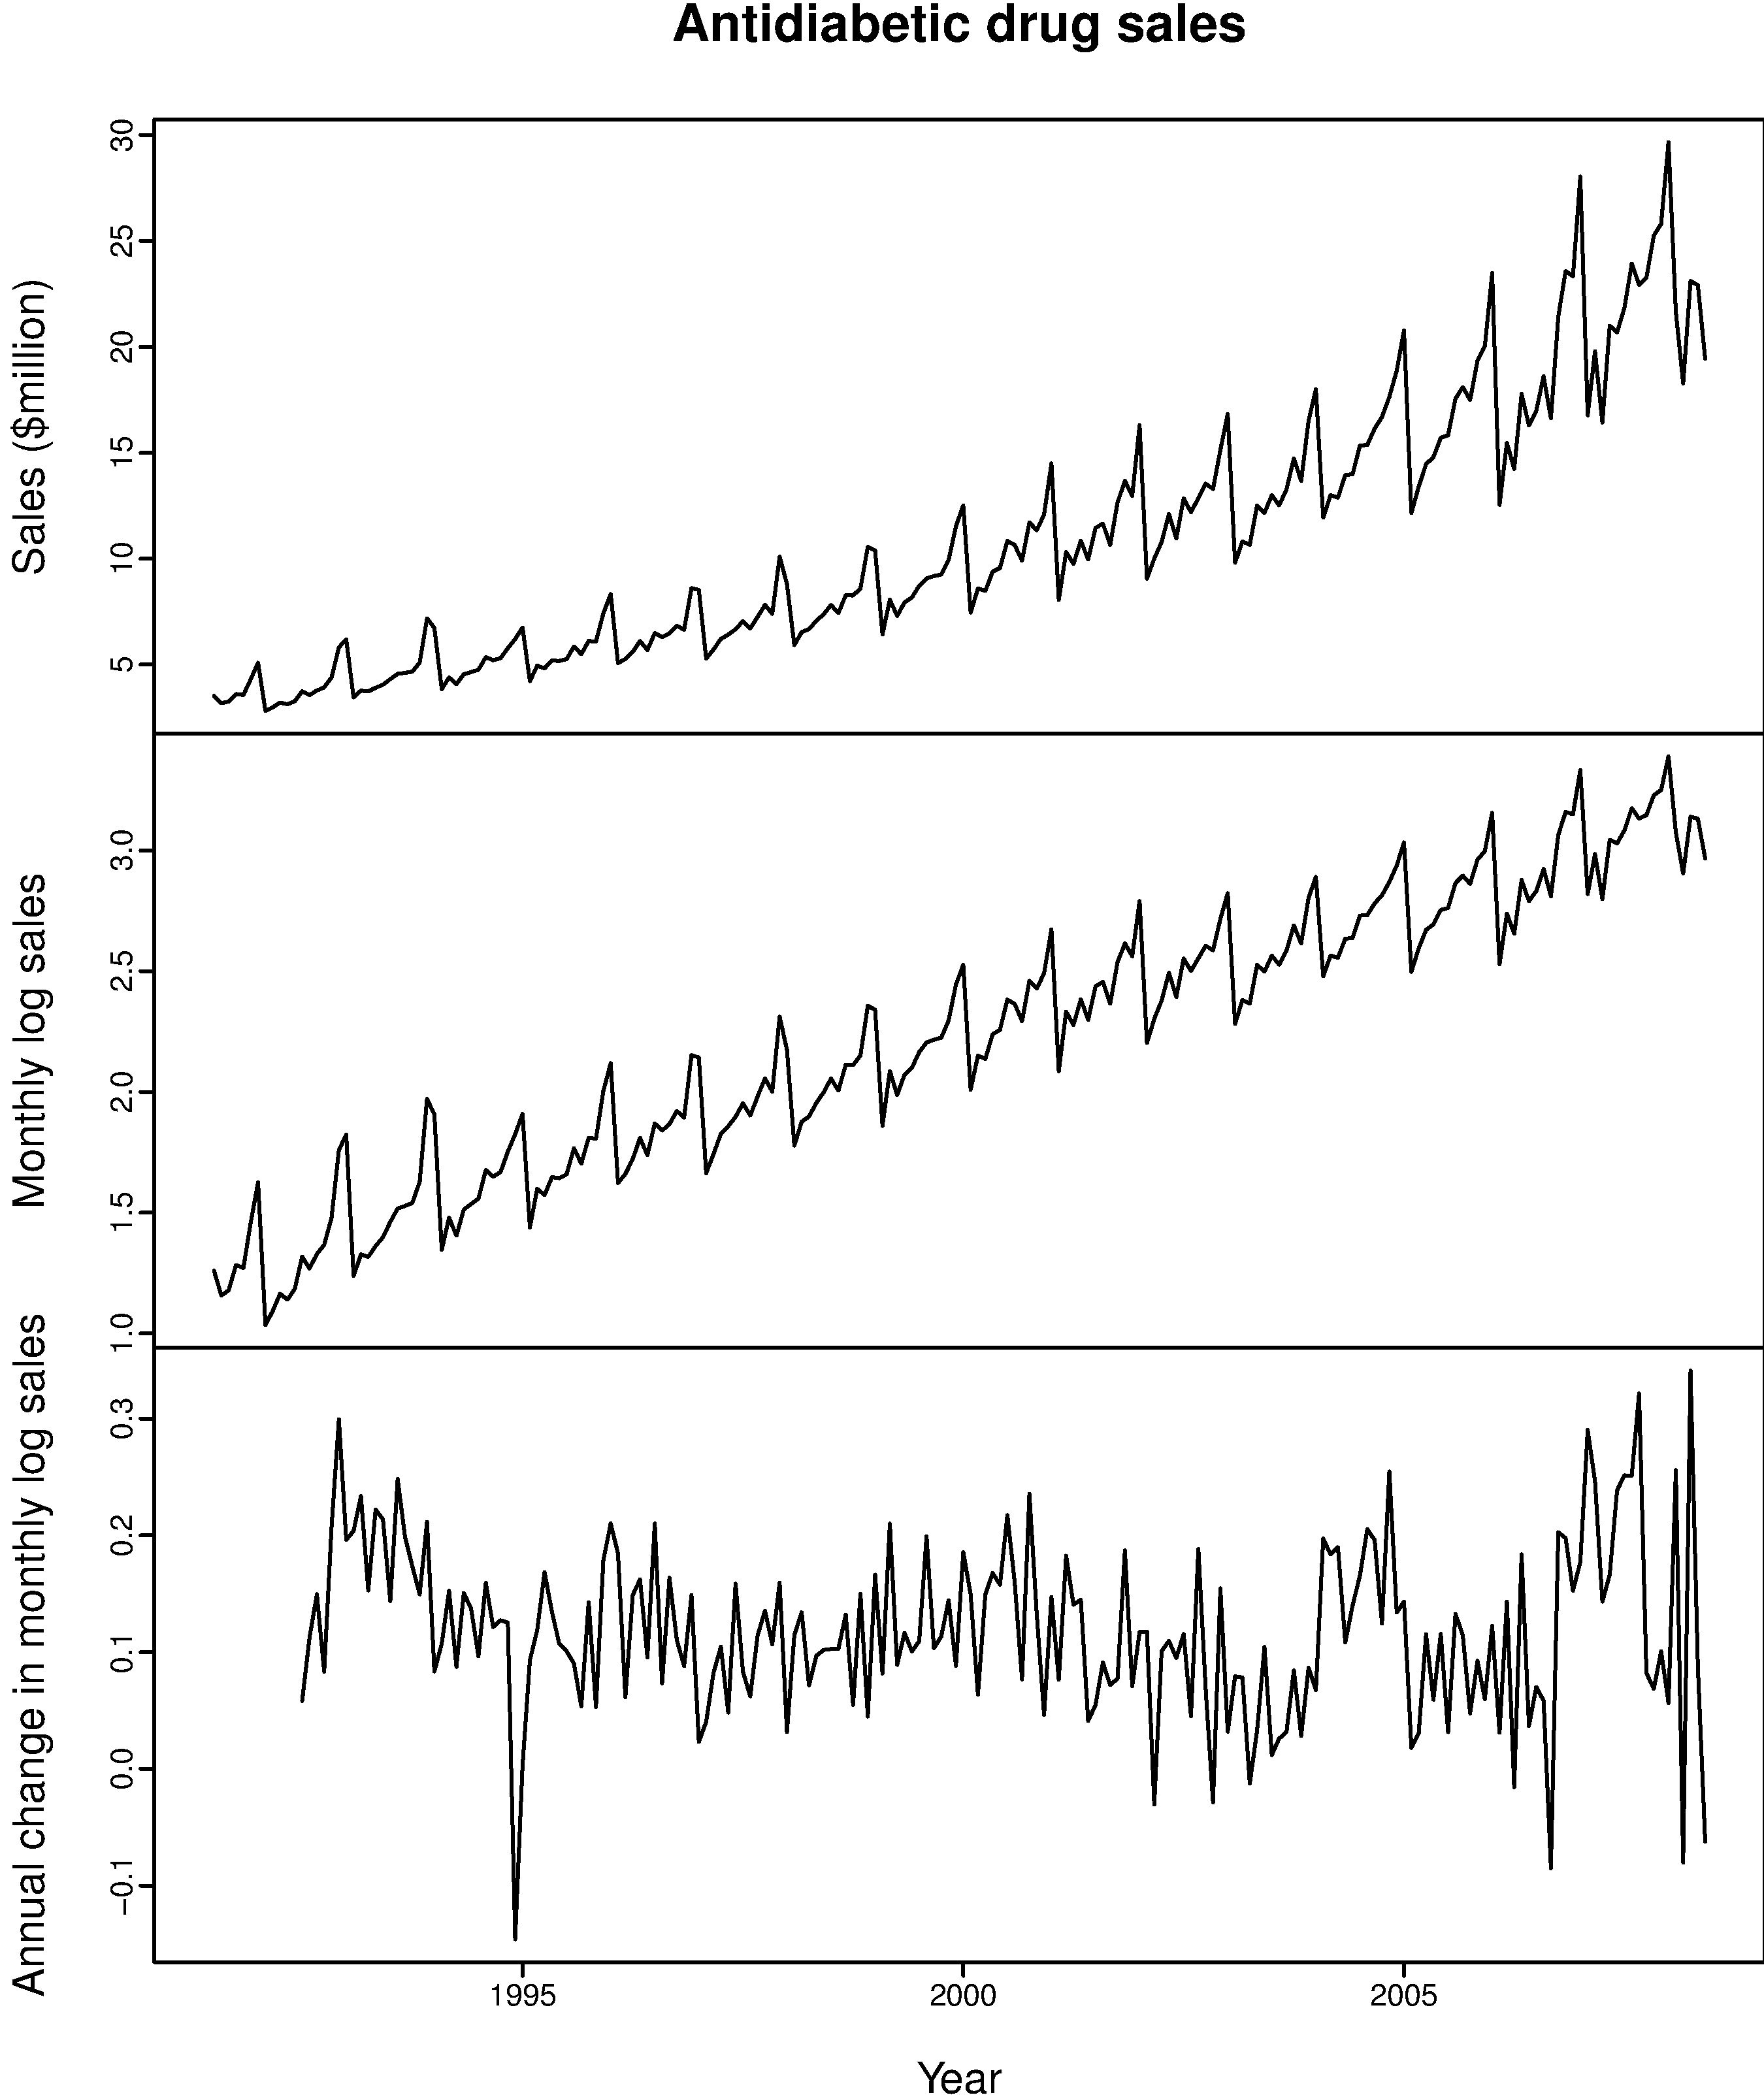
\includegraphics[height=0.7\textheight]{diffa10.png}
    	\end{center}
  
		
        Критерий~KPSS: для исходного ряда ${p<0.01},$ для логарифмированного~--- ${p<0.01},$ после сезонного дифференцирования~--- ${p>0.1}.$
	}
\end{frame}

\begin{frame}{Комбинированное дифференцирование}
	\only<1>{
		Сезонное и обычное дифференцирование может применяться к одному ряду в любом порядке.
		
		\bigskip
		
		Если ряд имеет выраженный сезонный профиль, рекомендуется начинать с сезонного дифференцирования~--- после него ряд уже может оказаться стационарным.
	}
	
	\only<2>{

    	\begin{center}
    		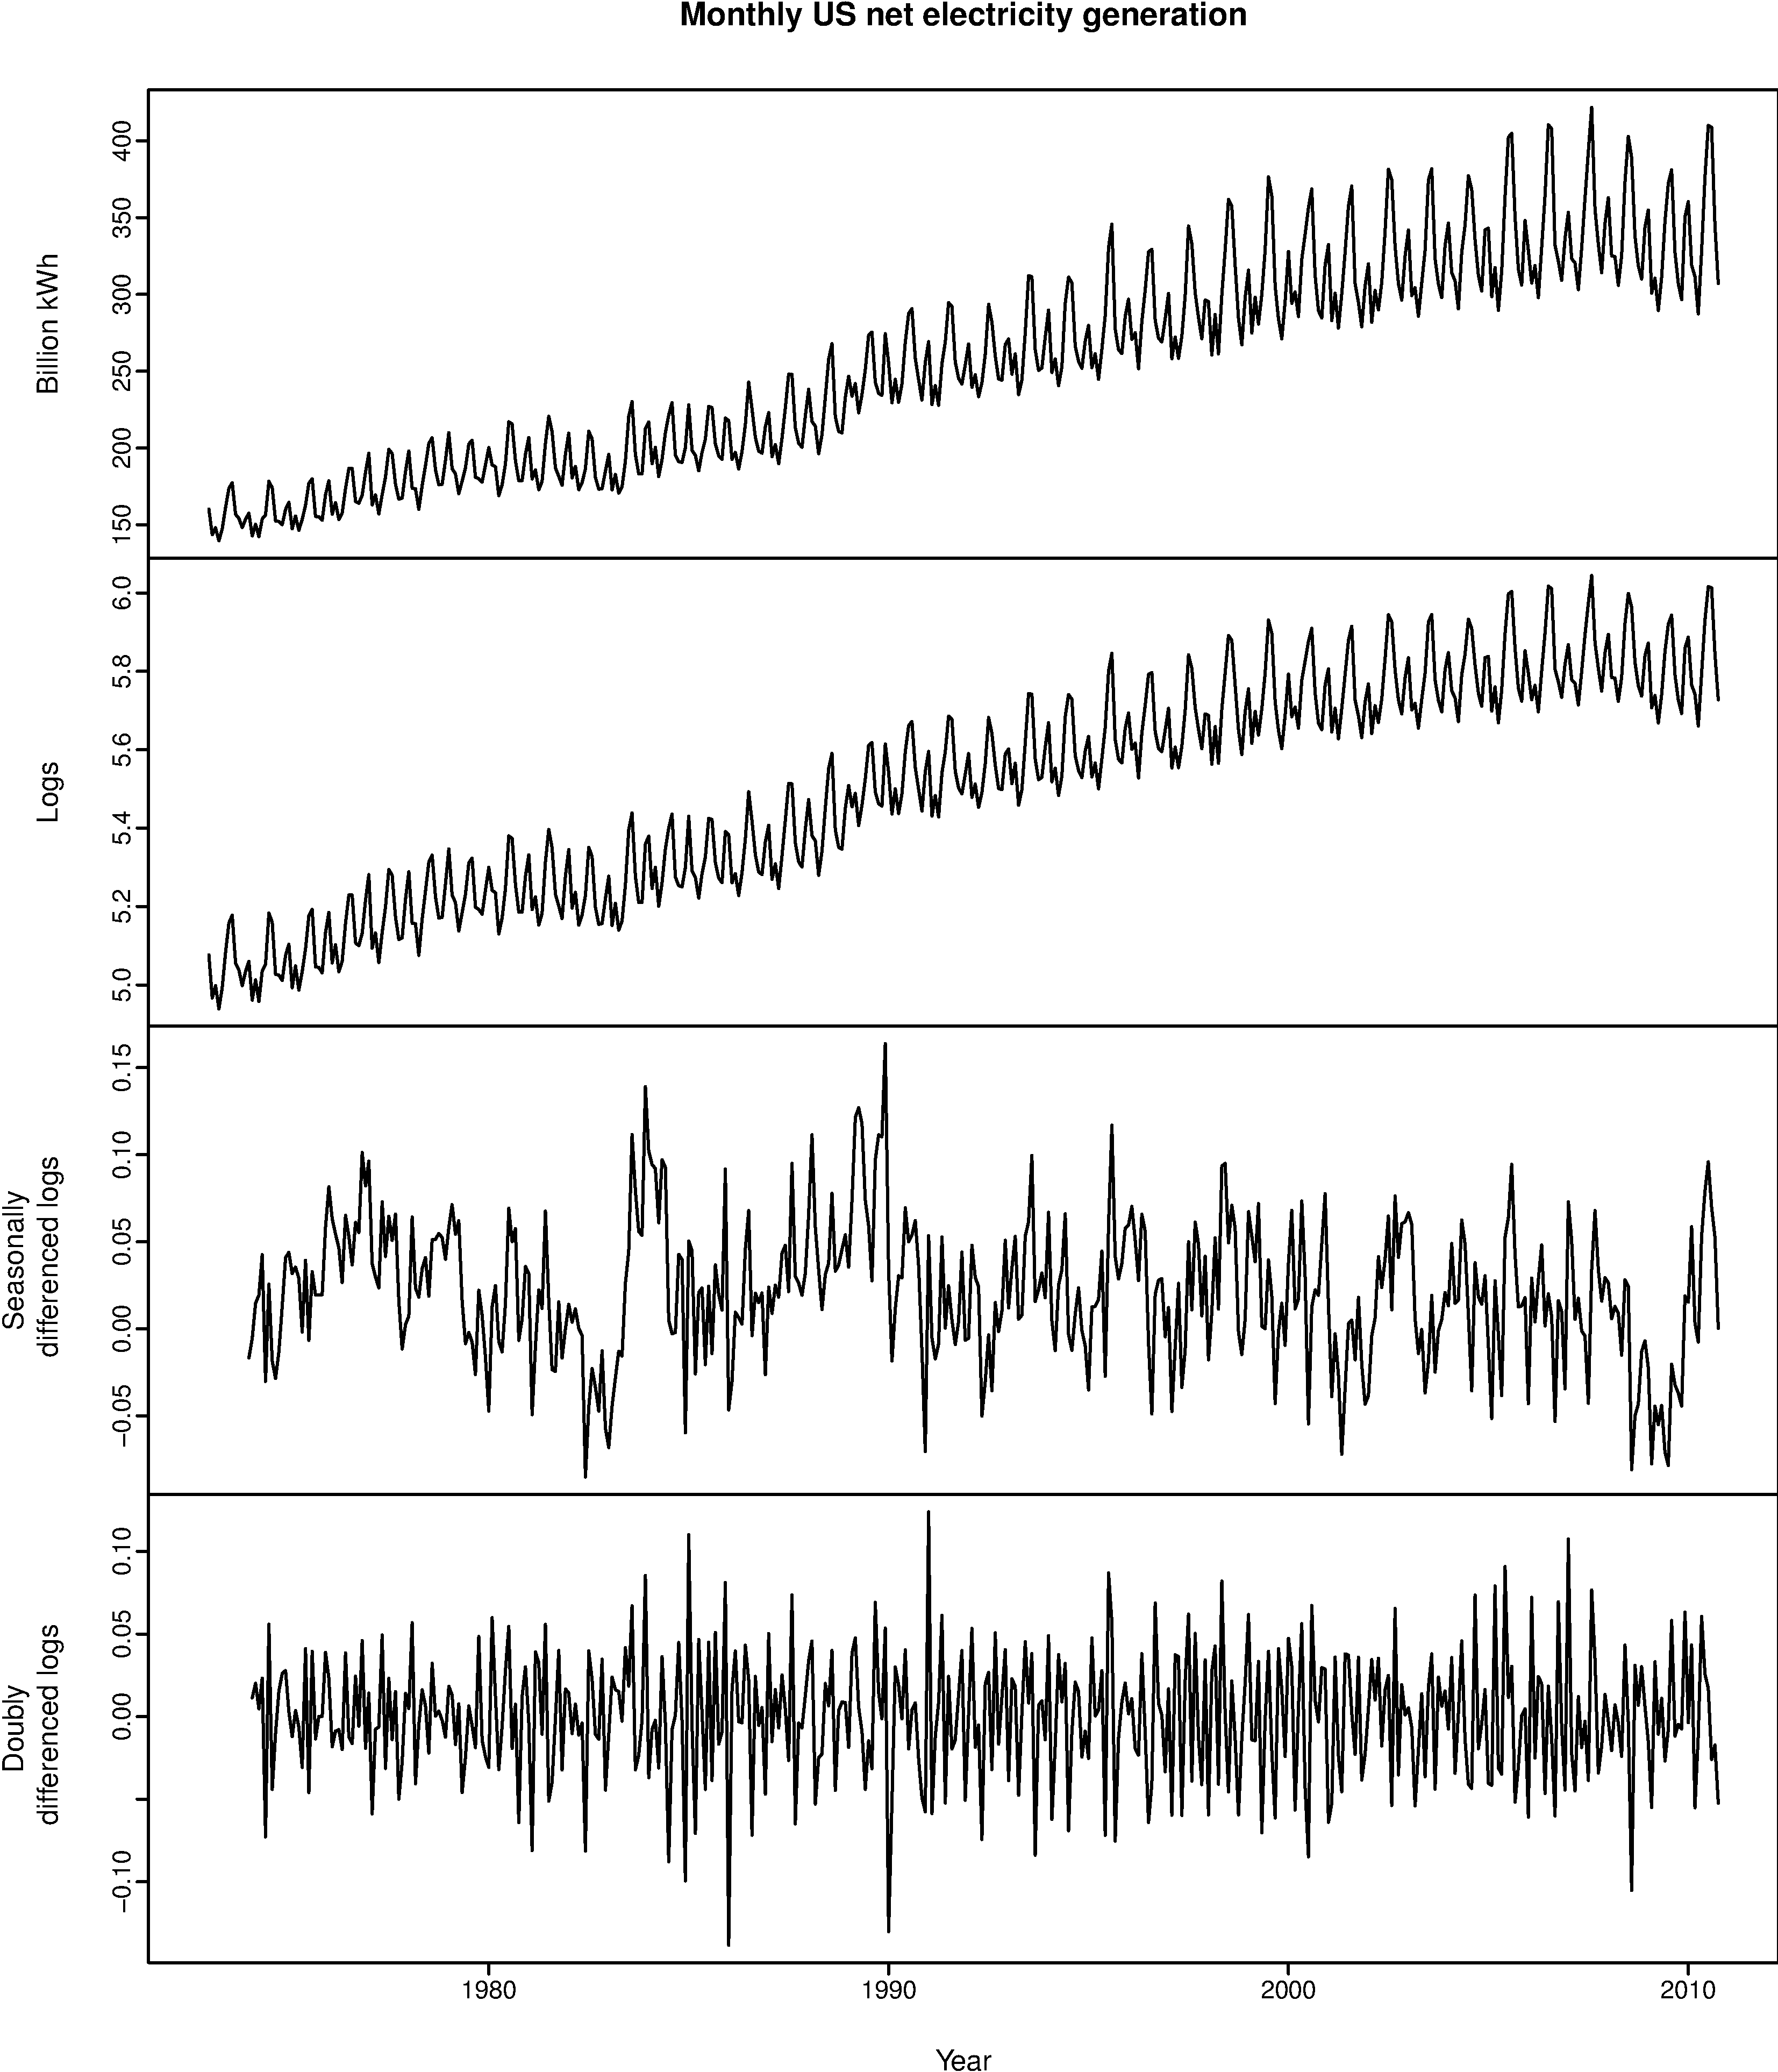
\includegraphics[height=0.6\textheight]{diffusnetelec.png}
    	\end{center}
  
        Критерий KPSS: для исходного ряда ${p<0.01},$ для логарифмированного~--- ${p<0.01},$ после сезонного дифференцирования~--- ${p=0.0355},$ после ещё одного дифференцирования~--- ${p>0.1}.$
	}
\end{frame}




\begin{frame}{Скользящее среднее}
%%%%%%%%%%%%%%%%%%%%%%%%%%%%%%%%%%%%%%%%%%%%%%%%%%%%%%%%%%%%%%%%%%%%%%%			
% Следующий класс моделей — это скользящее среднее. Чтобы лучше понимать, как они устроены, можно начать с рассмотрения независимого, одинаково распределённого во времени шума. Для каждого значения t можно вычислить среднее арифметическое между точками t и t-1. Также можно вычислять среднее не по двум, а по трём или четырём точкам. То, что получается в результате такого усреднения, — это уже не простая выборка с независимыми, одинаково распределёнными элементами. Соседние значения на красной линии очень похожи друг на друга, потому что в их вычислении используются одни и те же шумовые компоненты.
%%%%%%%%%%%%%%%%%%%%%%%%%%%%%%%%%%%%%%%%%%%%%%%%%%%%%%%%%%%%%%%%%%%%%%%			
	\only<1>{	
		Пусть у нас есть независимый одинаково распределённый во времени шум $\varepsilon_t$:
		\begin{center}
			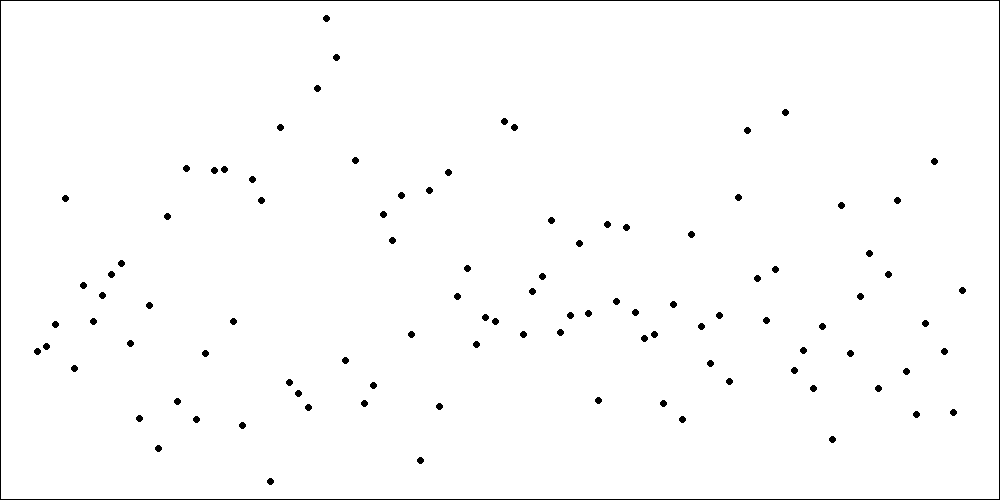
\includegraphics[width=0.8\textwidth]{MA1.png}
		\end{center}	
	}
	\only<2>{
		Среднее по двум соседним точкам:
		\begin{center}
			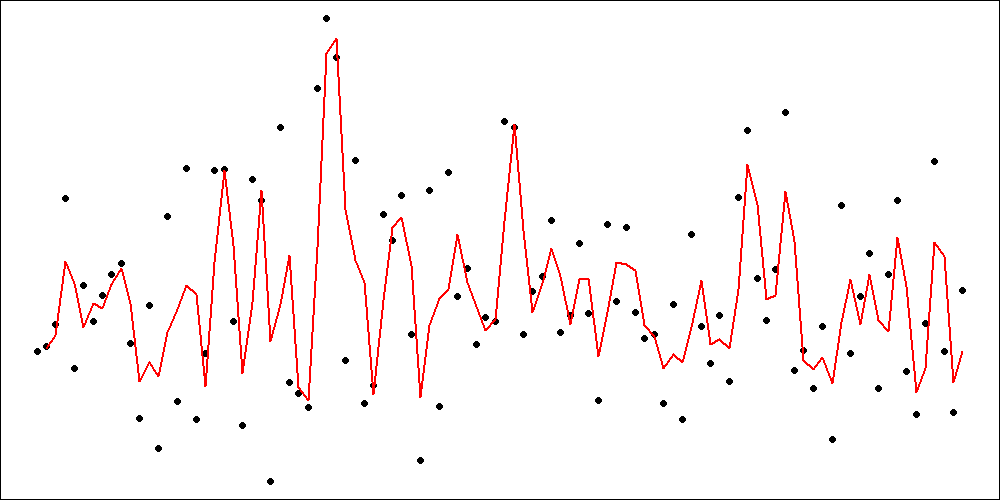
\includegraphics[width=0.8\textwidth]{MA2.png}
		\end{center}	
	}
	\only<3>{
		Среднее по трём соседним точкам:
		\begin{center}
			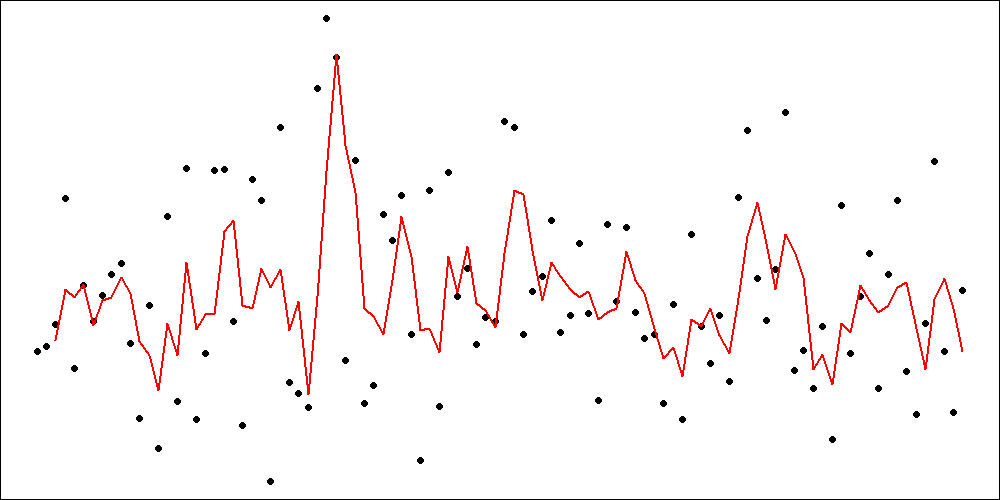
\includegraphics[width=0.8\textwidth]{MA3.png}
		\end{center}	
	}
	\only<4>{
		Среднее по четырём соседним точкам:
		\begin{center}
			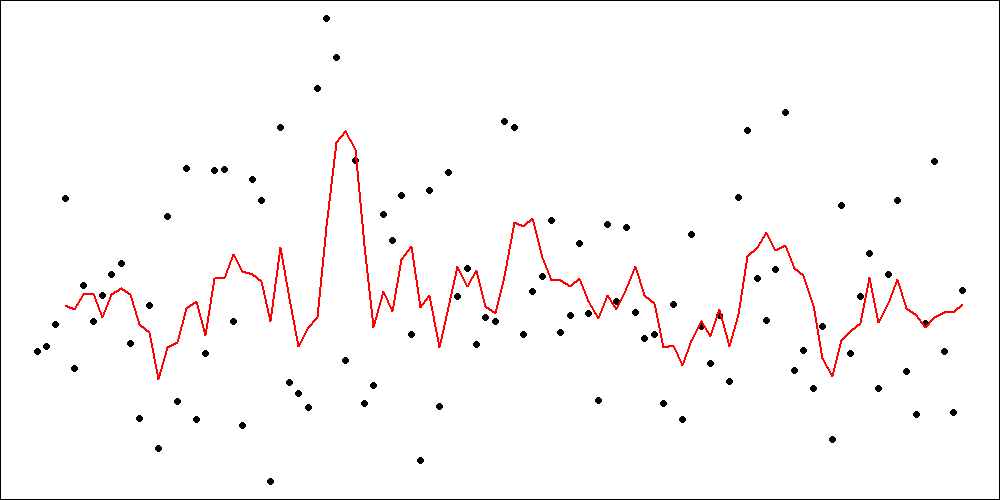
\includegraphics[width=0.8\textwidth]{MA4.png}
		\end{center}	
	}
	\end{frame}



\begin{frame}{Авторегрессия}
%%%%%%%%%%%%%%%%%%%%%%%%%%%%%%%%%%%%%%%%%%%%%%%%%%%%%%%%%%%%%%%%%%%%%%%			
% Ранее была предпринята попытка свести задачу прогнозирования временного ряда к задаче регрессии, выбирая какие-то признаки, зависящие от времени. Результат получился плохим, выбранных признаков явно недостаточно, нужны дополнительные. Можно перейти к следующей идее: делать регрессию для ряда не на какие-то внешние признаки, зависящие от времени, а на его собственные значения в прошлом. Такая модель называется моделью авторегрессии порядка p (AR(p)). В этой модели yt представляет собой линейную комбинацию p предыдущих значений ряда и шумовой компоненты.
%%%%%%%%%%%%%%%%%%%%%%%%%%%%%%%%%%%%%%%%%%%%%%%%%%%%%%%%%%%%%%%%%%%%%%%			
%    \only<1>{
    $$AR(p)\colon \;\;\; y_t = \phi_1 y_{t-1} + \phi_2 y_{t-2} + \dots + \phi_p y_{t-p} + \varepsilon_t,$$
    где $y_t$~--- стационарный ряд с нулевым средним, $\phi_1,\dots,\phi_p$~--- константы ($\phi_p \neq 0$), $\varepsilon_t$~--- гауссов белый шум с нулевым средним и постоянной дисперсией $\sigma_\varepsilon^2.$

    \bigskip

    Если среднее равно $\mu$, модель принимает вид
    $$y_t = \alpha + \phi_1y_{t-1} + \phi_2 y_{t-2} + \dots + \phi_p y_{t-p} + \varepsilon_t,$$
    где $\alpha=\mu\left(1-\phi_1-\dots-\phi_p\right).$

    \bigskip

    Другой способ записи:
    $$\phi\left(B\right)y_t = \left(1-\phi_1B - \phi_2B^2 - \dots - \phi_pB^p\right)y_t = \varepsilon_t,$$
    где $B$~--- разностный оператор ($By_t = y_{t-1}$).

    \bigskip

    Линейная комбинация $p$ подряд идущих членов ряда даёт белый шум.
%	}
%	
%	\only<2>{
%	Чтобы ряд AR(p) был стационарным, должны выполняться ограничения на коэффициенты.
%	Например,
%	\begin{itemize}
%		\item в AR(1) необходимо $-1<\phi_1<1$;
%		\item в AR(2) необходимо $-1<\phi_2<1, \;\phi_1+\phi_2<1,\; \phi_2-\phi_1<1$.
%	\end{itemize}
%	C ростом $p$ вид ограничений усложняется.		
%	}
\end{frame}

\section{ARIMA}
\subsection{Теория}

\begin{frame}{ARMA (Autogerressive moving average)}
%%%%%%%%%%%%%%%%%%%%%%%%%%%%%%%%%%%%%%%%%%%%%%%%%%%%%%%%%%%%%%%%%%%%%%%			
% Можно проделать следующий трюк: взять авторегрессионную модель порядка p и модель скользящего среднего порядка q и сложить то, что находится у них в правых частях. Результат — это модель ARMA(p, q). Главное, что нужно знать об этой модели: теорема Вольда утверждает, что любой стационарный временной ряд может быть описать моделью ARMA(p; q) с правильным подбором значений параметров p; q. Это прекрасный результат, который означает, что семейство моделей ARMA(p; q) достаточно богато для того, чтобы в нём можно было найти хорошую модель, описывающую любой стационарный ряд.
%%%%%%%%%%%%%%%%%%%%%%%%%%%%%%%%%%%%%%%%%%%%%%%%%%%%%%%%%%%%%%%%%%%%%%%			
    $$ARMA(p,q)\colon \;\; y_t = \phi_1 y_{t-1} + \dots + \phi_p y_{t-p} + \varepsilon_t + \theta_1\varepsilon_{t-1} + \theta_2\varepsilon_{t-2} + \dots + \theta_q \varepsilon_{t-q},$$
    где $y_t$~--- стационарный ряд с нулевым средним, $\phi_1,\dots,\phi_p,\theta_1,\dots,\theta_q$~--- константы ($\phi_p \neq 0$, $\theta_q\neq0$), $\varepsilon_t$~--- гауссов белый шум с нулевым средним и~постоянной дисперсией $\sigma_\varepsilon^2.$

    \bigskip

    Если среднее равно $\mu$, модель принимает вид
    $$y_t = \alpha + \phi_1y_{t-1} + \phi_2 y_{t-2} + \dots + \phi_p y_{t-p} + \varepsilon_t + \theta_1\varepsilon_{t-1} + \theta_2\varepsilon_{t-2} + \dots + \theta_q \varepsilon_{t-q},$$
    где $\alpha=\mu\left(1-\phi_1-\dots-\phi_p\right).$

    \bigskip

    Другой способ записи:
    $$\phi\left(B\right)y_t = \theta\left(B\right)\varepsilon_t.$$

    \bigskip

    Теорема Вольда: любой стационарный ряд может быть аппроксимирован моделью $ARMA(p,q)$ с любой точностью.
\end{frame}

\begin{frame}{ARIMA (Autogerressive integrated moving average)}
%%%%%%%%%%%%%%%%%%%%%%%%%%%%%%%%%%%%%%%%%%%%%%%%%%%%%%%%%%%%%%%%%%%%%%%			
% 1. Теорема Вольда: любой стационарный ряд может быть описан моделью ARMA(p; q) с любой наперёд заданной точностью.
% 2. При помощи дифференцирования нестационарный ряд можно сделать стационарным.
% Эти две идеи и лежат в основе моделей класса ARIMA. Модель ARIMA(p; d; q) — это модель ARMA(p; q) для d раз продифференцированного ряда.
%%%%%%%%%%%%%%%%%%%%%%%%%%%%%%%%%%%%%%%%%%%%%%%%%%%%%%%%%%%%%%%%%%%%%%%			
    Ряд описывается моделью $ARIMA(p,d,q),$ если ряд его разностей $$\nabla^d y_t = \left(1-B\right)^d y_t$$ описывается моделью $ARMA(p,q)$.

    $$\phi\left(B\right)\nabla^d y_t = \theta\left(B\right)\varepsilon_t.$$
\end{frame}

\subsection{Определение параметров моделей}
\begin{frame}{$\alpha, \phi, \theta$}
%%%%%%%%%%%%%%%%%%%%%%%%%%%%%%%%%%%%%%%%%%%%%%%%%%%%%%%%%%%%%%%%%%%%%%%			
% После изучения устройства моделей класса ARIMA настало время разобраться, как настраивать эти модели и получать с их помощью прогнозы. У моделей класса ARIMA есть несколько групп параметров. Параметры d;D; q; Q; p; P можно считать гиперпараметрами, поскольку они определяют структуру и количество коэффициентов в самой модели ARIMA. Остальные параметры являются коэффициентами в регрессионном уравнении.
% Если зафиксированы параметры d;D; q; Q; p; P, то есть зафиксирована структура модели ARIMA, то остальные параметры  можно подобрать с помощью метода наименьших квадратов. Фактически происходит настраивание привычной регрессии методом минимизации квадратичной ошибки.
% Единственный трюк заключается в определении коэффициентов тета, которые стоят при шумовых компонентах из прошлого. Наблюдать шумовые компоненты невозможно, поэтому, чтобы подставить их в регрессионное уравнение, их нужно предварительно оценить. Обычно оценка производится с помощью остатков от авторегрессии, которая предварительно строится по исследуемым данным.
% Если шум, который стоит в модели ARIMA, является белым (независимый, одинаково распределённый, гауссовский), то метод наименьших квадратов даёт оценки максимального правдоподобия для параметров альфа, фи и тета, а, значит, эти оценки обладают некоторыми хорошими свйоствами.
%%%%%%%%%%%%%%%%%%%%%%%%%%%%%%%%%%%%%%%%%%%%%%%%%%%%%%%%%%%%%%%%%%%%%%%			
	\begin{itemize}
		\item Если все остальные параметры фиксированы, коэффициенты регрессии подбираются методом наименьших квадратов
		\item Чтобы найти коэффициенты $\theta$, шумовая компонента предварительно оценивается с помощью остатков авторегрессии
		\item Если шум белый (независимый одинаково распределённый гауссовский), то МНК даёт оценки максимального правдоподобия
	\end{itemize}
\end{frame}

\begin{frame}{$d, D$}
%%%%%%%%%%%%%%%%%%%%%%%%%%%%%%%%%%%%%%%%%%%%%%%%%%%%%%%%%%%%%%%%%%%%%%%			
% Параметры d;D, которые задают порядки дифференцирования, необходимо подбирать так, чтобы ряд стал стационарным. Ранее уже упоминалось, что всегда рекомендуется начинать с сезонного дифференцирования, потому что уже после него ряд может оказаться стационарным. Дело в том, что выгодно дифференцировать ряд как можно меньше раз, потому что с увеличением количества дифференцирований растёт дисперсия итогового прогноза.
%%%%%%%%%%%%%%%%%%%%%%%%%%%%%%%%%%%%%%%%%%%%%%%%%%%%%%%%%%%%%%%%%%%%%%%			
	\begin{itemize}
		\item Порядки дифференцирования подбираются так, чтобы ряд стал стационарным
		\item Ещё раз: если ряд сезонный, рекомендуется начинать с сезонного дифференцирования
		\item Чем меньше раз мы продифференцируем, тем меньше будет дисперсия итогового прогноза
	\end{itemize}
\end{frame}

\begin{frame}{$q, Q, p, P$}
%%%%%%%%%%%%%%%%%%%%%%%%%%%%%%%%%%%%%%%%%%%%%%%%%%%%%%%%%%%%%%%%%%%%%%%			
% К сожалению, гиперпараметры q; Q; p; P нельзя выбирать из принципа максимума правдоподобия. Например, чем больше значение параметра p, тем больше авторегрессионных компонент в итоговом уравнении, тем больше параметров фи и тем лучше это уравнение описывает данные. Чем больше значения гиперпараметров, тем больше параметров в модели и тем она сложнее. Таким образом, с увеличением значения этих гиперпараметров значение правдоподобия может только увеличиваться. Поэтому для сравнения моделей с разным количеством параметров необходим другой критерий, например, критерий Акаике.
% Оптимальной по критерию Акаике будет модель с наименьшим значением этого критерия. Такая модель, с одной стороны, будет достаточно хорошо описывать данные, а с другой — содержать не слишком большое количество параметров. В конечном итоге значения параметров q; Q; p; P определяются перебором: из разных значений гиперпараметров выбираются те, у которых значение критерия Акаике будет минимальным. Начальные приближения для этого перебора можно выбрать с помощью автокорреляционной функции.
%%%%%%%%%%%%%%%%%%%%%%%%%%%%%%%%%%%%%%%%%%%%%%%%%%%%%%%%%%%%%%%%%%%%%%%			
	\begin{itemize}
		\item Гиперпараметры нельзя выбирать из принципа максимума правдоподобия: $L$~всегда увеличивается с~их ростом
		\item Для сравнения моделей с разными $q, Q, p, P$ можно использовать информационные критерии
		\item Начальные приближения можно выбрать с помощью автокорреляций
	\end{itemize}
\end{frame}

\begin{frame}{Автокорреляционная функция (ACF)}
%%%%%%%%%%%%%%%%%%%%%%%%%%%%%%%%%%%%%%%%%%%%%%%%%%%%%%%%%%%%%%%%%%%%%%%
% Одной из важнейших характеристик временного ряда является автокорреляция, измеряющая в каком-то смысле сходство между значениями ряда в соседних точках. Автокорреляция — это уже встречавшаяся ранее корреляция Пирсона между исходным рядом и его версией, сдвинутой на несколько отсчётов. Количество отсчётов, на которое сдвинут ряд, называется лагом автокорреляции. Значения, принимаемые автокорреляцией такие же, как и у коэффициента Пирсона: [-1; 1]. Проверить, значимо ли отличие автокорреляции от нуля, можно с помощью такого же критерия Стьюдента, как используется для корреляции Пирсона.
%%%%%%%%%%%%%%%%%%%%%%%%%%%%%%%%%%%%%%%%%%%%%%%%%%%%%%%%%%%%%%%%%%%%%%%
	\only<1>{
	Наблюдения временного ряда автокоррелированы.
	
	\bigskip	
		
		\textbf{Автокорреляция:}
		$$r_\tau = r_{y_t y_{t+\tau}} = \frac{\sum\limits_{t=1}^{T-\tau} \left(y_t - \bar{y}\right)\left(y_{t+\tau} - \bar{y}\right) }{ \sum\limits_{t=1}^T \left(y_t - \bar{y}\right)^2 },\;\; \bar{y} = \frac1{T} \sum_{t=1}^T y_t.$$
		
		$r_\tau \in\left[-1,1\right], \;\; \tau$~--- лаг автокорреляции.
		
		\bigskip
		
		Проверка значимости отличия автокорреляции от нуля:
		\begin{center}
			\begin{tabular}{rl}
				временной ряд:                  & $Y^T = Y_1,\dots,Y_T;$ \\
				нулевая гипотеза:               & $H_0\colon r_\tau=0;$ \\
				альтернатива:                   & $H_1\colon r_\tau\neq0;$ \\
				статистика:                     & $T\left(Y^T\right) = \frac{r_{\tau} \sqrt{T-\tau-2}}{\sqrt{1-r_\tau^2}};$ \\
				нулевое распределение:          & $St\left(T-\tau-2\right)$.\\
			\end{tabular}
		\end{center}
	}
	
			
	
\end{frame}


\begin{frame}{Частичная автокорреляционная функция (PACF)}
	\textbf{Частичная автокорреляция} стационарного ряда $y_t$~--- автокорреляция остатков авторегрессии предыдущего порядка:
	$$\phi_{hh} = \begin{cases}
	r\left(y_{t+1},y_t\right), & h=1, \\
	r\left(y_{t+h} - \hat{y}_{t+h}, y_{t} - \hat{y}_t\right), & h\geq 2,
	\end{cases}
	$$
	где $\hat{y}_{t+h}$ и $\hat{y}_{t}$~--- предсказания регрессий $y_{t+h}$ и $y_{t}$ на $y_{t+1}, y_{t+2}, \dots, y_{t+h-1}$:
	\begin{align*}
	\hat{y}_t     &= \beta_1y_{t+1} +\beta_2y_{t+2} + \dots + \beta_{h-1} y_{t+h-1}, \\
	\hat{y}_{t+h} &= \beta_1y_{t+h-1} +\beta_2y_{t+h-2} + \dots + \beta_{h-1} y_{t+1}. \\
	\end{align*}	
\end{frame}

\begin{frame}{$q, Q, p, P$}
\begin{itemize}
	\item В модели $ARIMA(p,d,0)$ ACF экспоненциально затухает или имеет синусоидальный вид, а PACF значимо отличается от нуля при лаге $p$
	\item В модели $ARIMA(0,d,q)$ PACF экспоненциально затухает или имеет синусоидальный вид, а ACF значимо отличается от нуля при лаге $q$
\end{itemize}

$\Rightarrow$ начальные приближения для $p,q,P,Q$:

\begin{itemize}
	\item $q$: номер последнего лага $\tau<S$, при котором автокорреляция значима	
	\item $p$: номер последнего лага $\tau<S$, при котором частичная автокорреляция значима		
\end{itemize}
\end{frame}

\subsection{Прогнозирование}
\begin{frame}{Прогнозирование с помощью ARIMA}
	\only<1>{
		\begin{enumerate}
			\item Строится график ряда, идентифицируются необычные значения.
			\item При необходимости делается стабилизирующее дисперсию преобразование.
			\item Если ряд нестационарен, подбирается порядок дифференцирования.
			\item Анализируются ACF/PACF, чтобы понять, можно ли использовать модели AR(p)/MA(q).
			\item Обучаются модели-кандидаты, сравнивается их AIC/AICc.
			\item Остатки полученной модели исследуются на несмещённость, стационарность и неавтокоррелированность; если предположения не~выполняются, исследуются модификации модели.
			\item В финальной модели $t$ заменяется на $T+h$, будущие наблюдения~--- на их прогнозы, будущие ошибки~--- на нули, прошлые ошибки~--- на~остатки.
		\end{enumerate}
	}
\end{frame}

\section{}
\begin{frame}{Литература}
	Hyndman R.J., Athanasopoulos G. \textit{Forecasting: principles and practice}. --- OTexts, \url{https://www.otexts.org/book/fpp}
\end{frame}
\end{document}
